% Options for packages loaded elsewhere
\PassOptionsToPackage{unicode}{hyperref}
\PassOptionsToPackage{hyphens}{url}
%
\documentclass[
  11pt,
]{article}
\usepackage[]{mathpazo}
\usepackage{amssymb,amsmath}
\usepackage{ifxetex,ifluatex}
\ifnum 0\ifxetex 1\fi\ifluatex 1\fi=0 % if pdftex
  \usepackage[T1]{fontenc}
  \usepackage[utf8]{inputenc}
  \usepackage{textcomp} % provide euro and other symbols
\else % if luatex or xetex
  \usepackage{unicode-math}
  \defaultfontfeatures{Scale=MatchLowercase}
  \defaultfontfeatures[\rmfamily]{Ligatures=TeX,Scale=1}
\fi
% Use upquote if available, for straight quotes in verbatim environments
\IfFileExists{upquote.sty}{\usepackage{upquote}}{}
\IfFileExists{microtype.sty}{% use microtype if available
  \usepackage[]{microtype}
  \UseMicrotypeSet[protrusion]{basicmath} % disable protrusion for tt fonts
}{}
\makeatletter
\@ifundefined{KOMAClassName}{% if non-KOMA class
  \IfFileExists{parskip.sty}{%
    \usepackage{parskip}
  }{% else
    \setlength{\parindent}{0pt}
    \setlength{\parskip}{6pt plus 2pt minus 1pt}}
}{% if KOMA class
  \KOMAoptions{parskip=half}}
\makeatother
\usepackage{xcolor}
\IfFileExists{xurl.sty}{\usepackage{xurl}}{} % add URL line breaks if available
\IfFileExists{bookmark.sty}{\usepackage{bookmark}}{\usepackage{hyperref}}
\hypersetup{
  pdftitle={ST422 Assignment},
  pdfauthor={23074},
  hidelinks,
  pdfcreator={LaTeX via pandoc}}
\urlstyle{same} % disable monospaced font for URLs
\usepackage[margin=1in]{geometry}
\usepackage{color}
\usepackage{fancyvrb}
\newcommand{\VerbBar}{|}
\newcommand{\VERB}{\Verb[commandchars=\\\{\}]}
\DefineVerbatimEnvironment{Highlighting}{Verbatim}{commandchars=\\\{\}}
% Add ',fontsize=\small' for more characters per line
\usepackage{framed}
\definecolor{shadecolor}{RGB}{248,248,248}
\newenvironment{Shaded}{\begin{snugshade}}{\end{snugshade}}
\newcommand{\AlertTok}[1]{\textcolor[rgb]{0.94,0.16,0.16}{#1}}
\newcommand{\AnnotationTok}[1]{\textcolor[rgb]{0.56,0.35,0.01}{\textbf{\textit{#1}}}}
\newcommand{\AttributeTok}[1]{\textcolor[rgb]{0.77,0.63,0.00}{#1}}
\newcommand{\BaseNTok}[1]{\textcolor[rgb]{0.00,0.00,0.81}{#1}}
\newcommand{\BuiltInTok}[1]{#1}
\newcommand{\CharTok}[1]{\textcolor[rgb]{0.31,0.60,0.02}{#1}}
\newcommand{\CommentTok}[1]{\textcolor[rgb]{0.56,0.35,0.01}{\textit{#1}}}
\newcommand{\CommentVarTok}[1]{\textcolor[rgb]{0.56,0.35,0.01}{\textbf{\textit{#1}}}}
\newcommand{\ConstantTok}[1]{\textcolor[rgb]{0.00,0.00,0.00}{#1}}
\newcommand{\ControlFlowTok}[1]{\textcolor[rgb]{0.13,0.29,0.53}{\textbf{#1}}}
\newcommand{\DataTypeTok}[1]{\textcolor[rgb]{0.13,0.29,0.53}{#1}}
\newcommand{\DecValTok}[1]{\textcolor[rgb]{0.00,0.00,0.81}{#1}}
\newcommand{\DocumentationTok}[1]{\textcolor[rgb]{0.56,0.35,0.01}{\textbf{\textit{#1}}}}
\newcommand{\ErrorTok}[1]{\textcolor[rgb]{0.64,0.00,0.00}{\textbf{#1}}}
\newcommand{\ExtensionTok}[1]{#1}
\newcommand{\FloatTok}[1]{\textcolor[rgb]{0.00,0.00,0.81}{#1}}
\newcommand{\FunctionTok}[1]{\textcolor[rgb]{0.00,0.00,0.00}{#1}}
\newcommand{\ImportTok}[1]{#1}
\newcommand{\InformationTok}[1]{\textcolor[rgb]{0.56,0.35,0.01}{\textbf{\textit{#1}}}}
\newcommand{\KeywordTok}[1]{\textcolor[rgb]{0.13,0.29,0.53}{\textbf{#1}}}
\newcommand{\NormalTok}[1]{#1}
\newcommand{\OperatorTok}[1]{\textcolor[rgb]{0.81,0.36,0.00}{\textbf{#1}}}
\newcommand{\OtherTok}[1]{\textcolor[rgb]{0.56,0.35,0.01}{#1}}
\newcommand{\PreprocessorTok}[1]{\textcolor[rgb]{0.56,0.35,0.01}{\textit{#1}}}
\newcommand{\RegionMarkerTok}[1]{#1}
\newcommand{\SpecialCharTok}[1]{\textcolor[rgb]{0.00,0.00,0.00}{#1}}
\newcommand{\SpecialStringTok}[1]{\textcolor[rgb]{0.31,0.60,0.02}{#1}}
\newcommand{\StringTok}[1]{\textcolor[rgb]{0.31,0.60,0.02}{#1}}
\newcommand{\VariableTok}[1]{\textcolor[rgb]{0.00,0.00,0.00}{#1}}
\newcommand{\VerbatimStringTok}[1]{\textcolor[rgb]{0.31,0.60,0.02}{#1}}
\newcommand{\WarningTok}[1]{\textcolor[rgb]{0.56,0.35,0.01}{\textbf{\textit{#1}}}}
\usepackage{longtable,booktabs}
% Correct order of tables after \paragraph or \subparagraph
\usepackage{etoolbox}
\makeatletter
\patchcmd\longtable{\par}{\if@noskipsec\mbox{}\fi\par}{}{}
\makeatother
% Allow footnotes in longtable head/foot
\IfFileExists{footnotehyper.sty}{\usepackage{footnotehyper}}{\usepackage{footnote}}
\makesavenoteenv{longtable}
\usepackage{graphicx,grffile}
\makeatletter
\def\maxwidth{\ifdim\Gin@nat@width>\linewidth\linewidth\else\Gin@nat@width\fi}
\def\maxheight{\ifdim\Gin@nat@height>\textheight\textheight\else\Gin@nat@height\fi}
\makeatother
% Scale images if necessary, so that they will not overflow the page
% margins by default, and it is still possible to overwrite the defaults
% using explicit options in \includegraphics[width, height, ...]{}
\setkeys{Gin}{width=\maxwidth,height=\maxheight,keepaspectratio}
% Set default figure placement to htbp
\makeatletter
\def\fps@figure{htbp}
\makeatother
\setlength{\emergencystretch}{3em} % prevent overfull lines
\providecommand{\tightlist}{%
  \setlength{\itemsep}{0pt}\setlength{\parskip}{0pt}}
\setcounter{secnumdepth}{5}

\title{ST422 Assignment}
\author{23074}
\date{December 08, 2020}

\begin{document}
\maketitle

{
\setcounter{tocdepth}{3}
\tableofcontents
}
\newpage

\hypertarget{q1-q2}{%
\section{Q1 \& Q2}\label{q1-q2}}

\hypertarget{sunshine-series}{%
\subsection{Sunshine series}\label{sunshine-series}}

\hypertarget{preliminary-analysis}{%
\subsubsection{Preliminary analysis}\label{preliminary-analysis}}

\begin{figure}
\centering
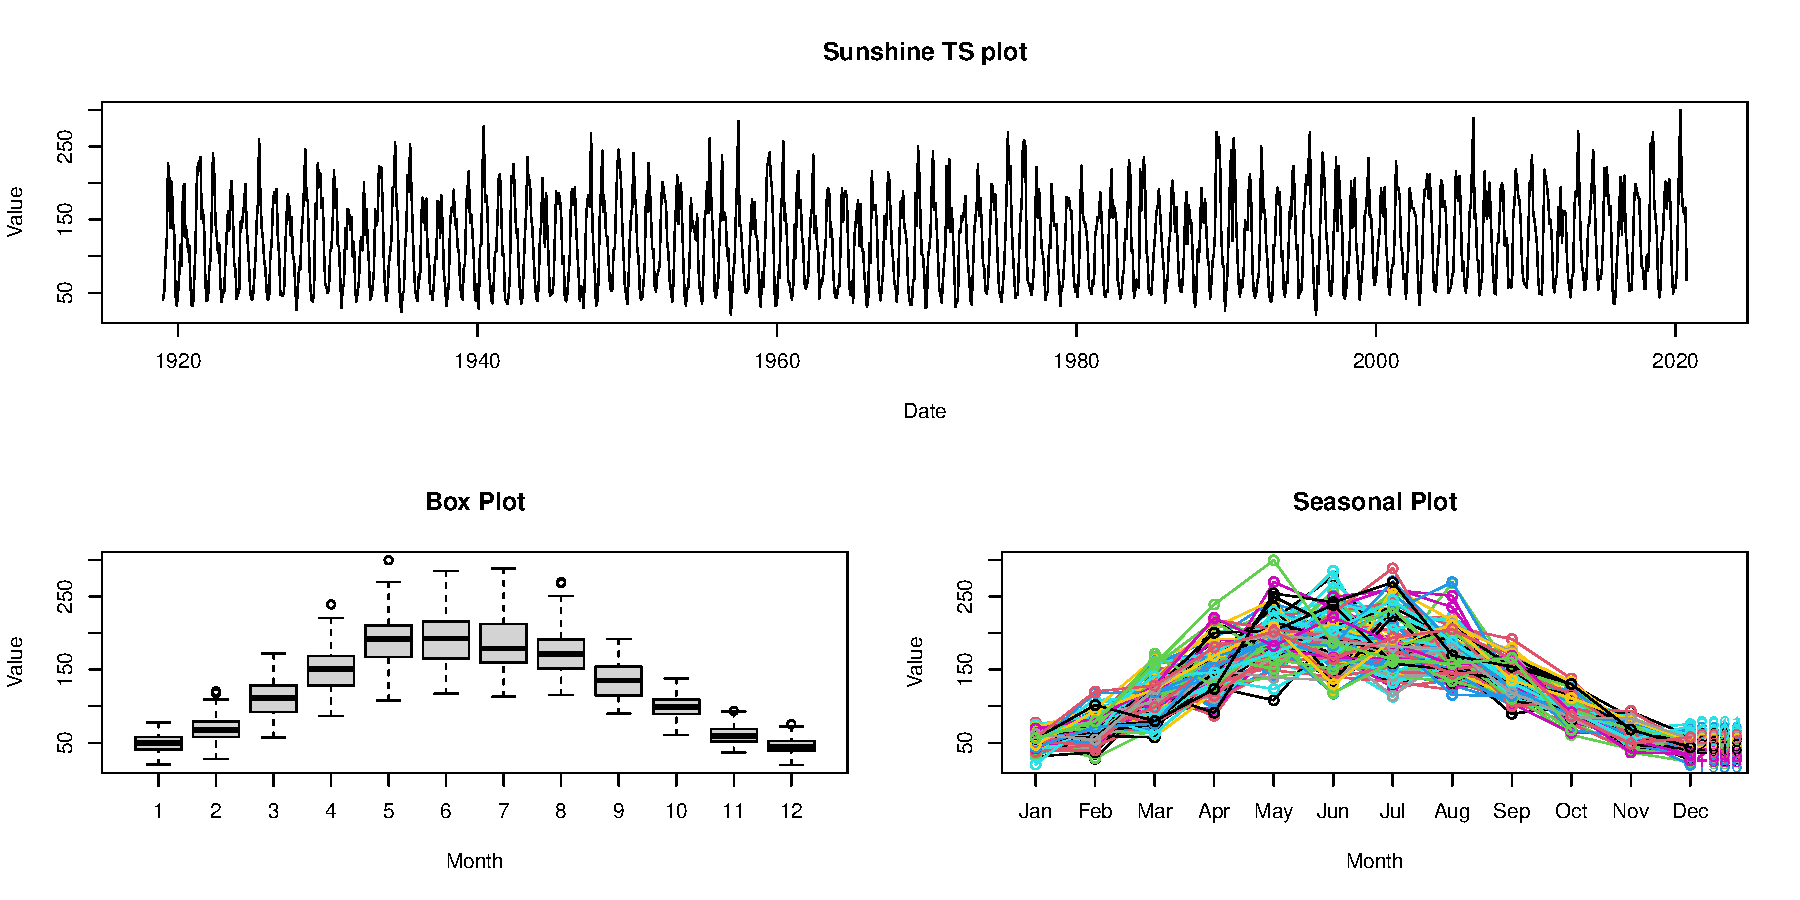
\includegraphics{ST422_files/figure-latex/unnamed-chunk-4-1.pdf}
\caption{Preliminary analysis on entire Sunshine series}
\end{figure}

\begin{figure}
\centering
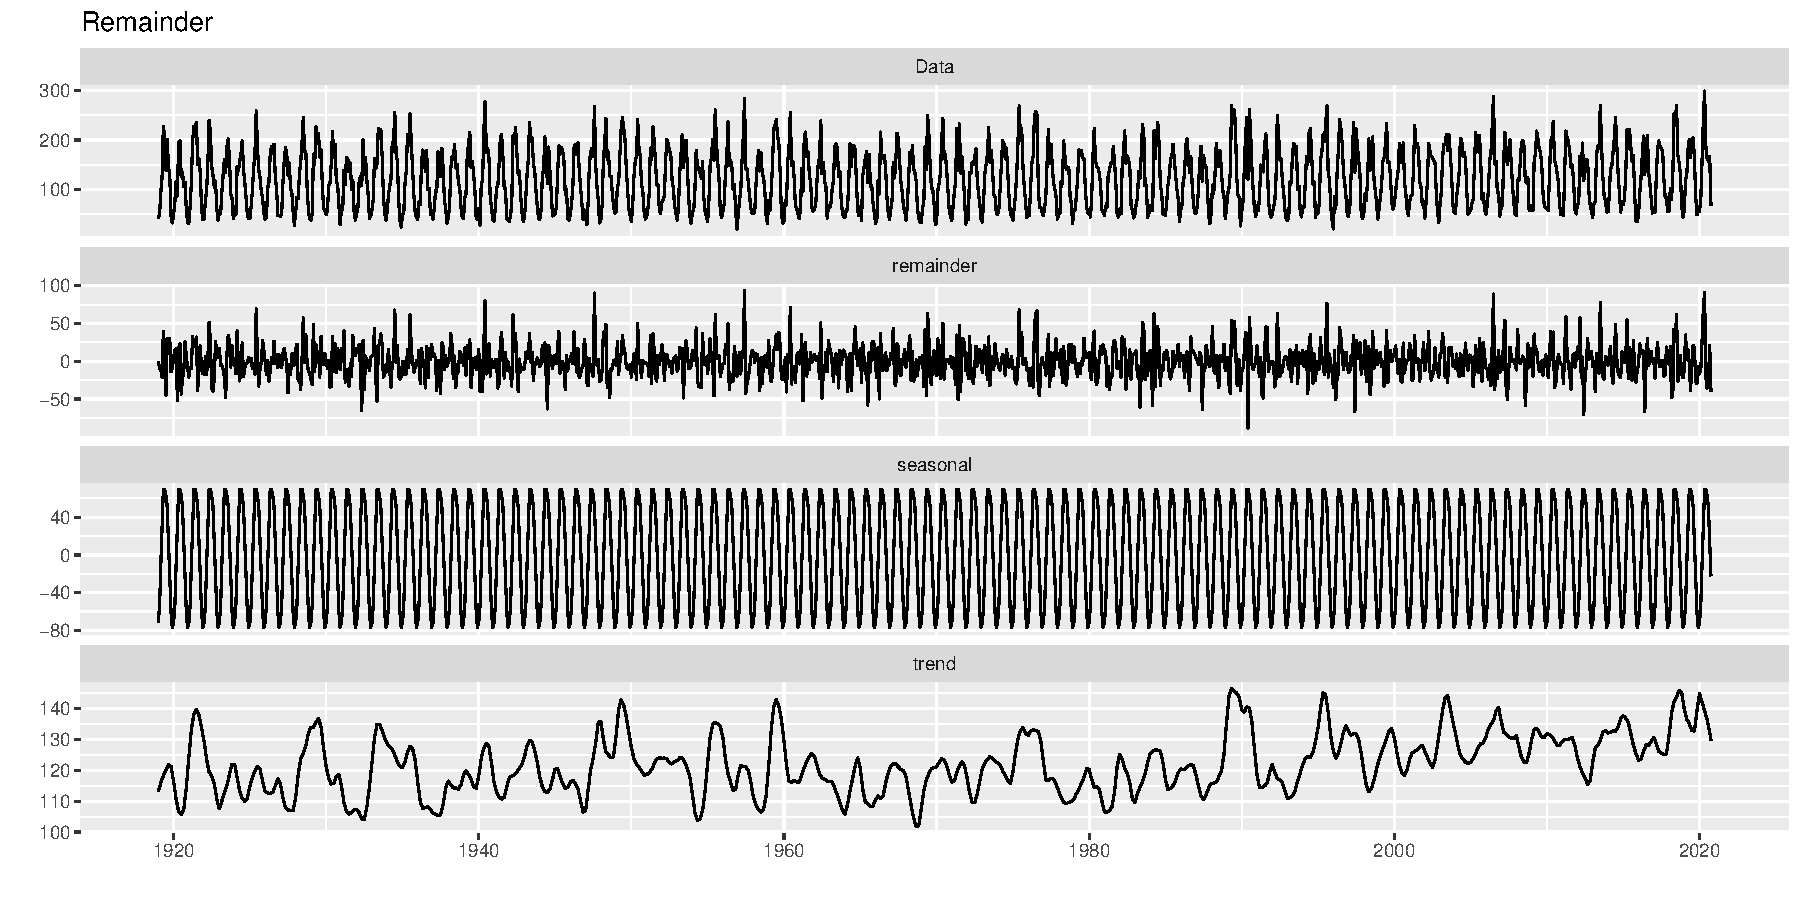
\includegraphics{ST422_files/figure-latex/unnamed-chunk-5-1.pdf}
\caption{Decomposition analysis on entire Sunshine series}
\end{figure}

By comparing the preliminary analysis based on the entire dataset
(Figure 1) and partial dataset (Figure 3), using the entire dataset is a
bit of stretch and there is no major difference in terms of the unique
patterns and trends observed between these two datasets. Hence, for
better intuitive understanding on analysis, the preliminary analysis is
conducted on the partial dataset (21st century) but the final modelling
will be using the entire population.

\newpage

\begin{figure}
\centering
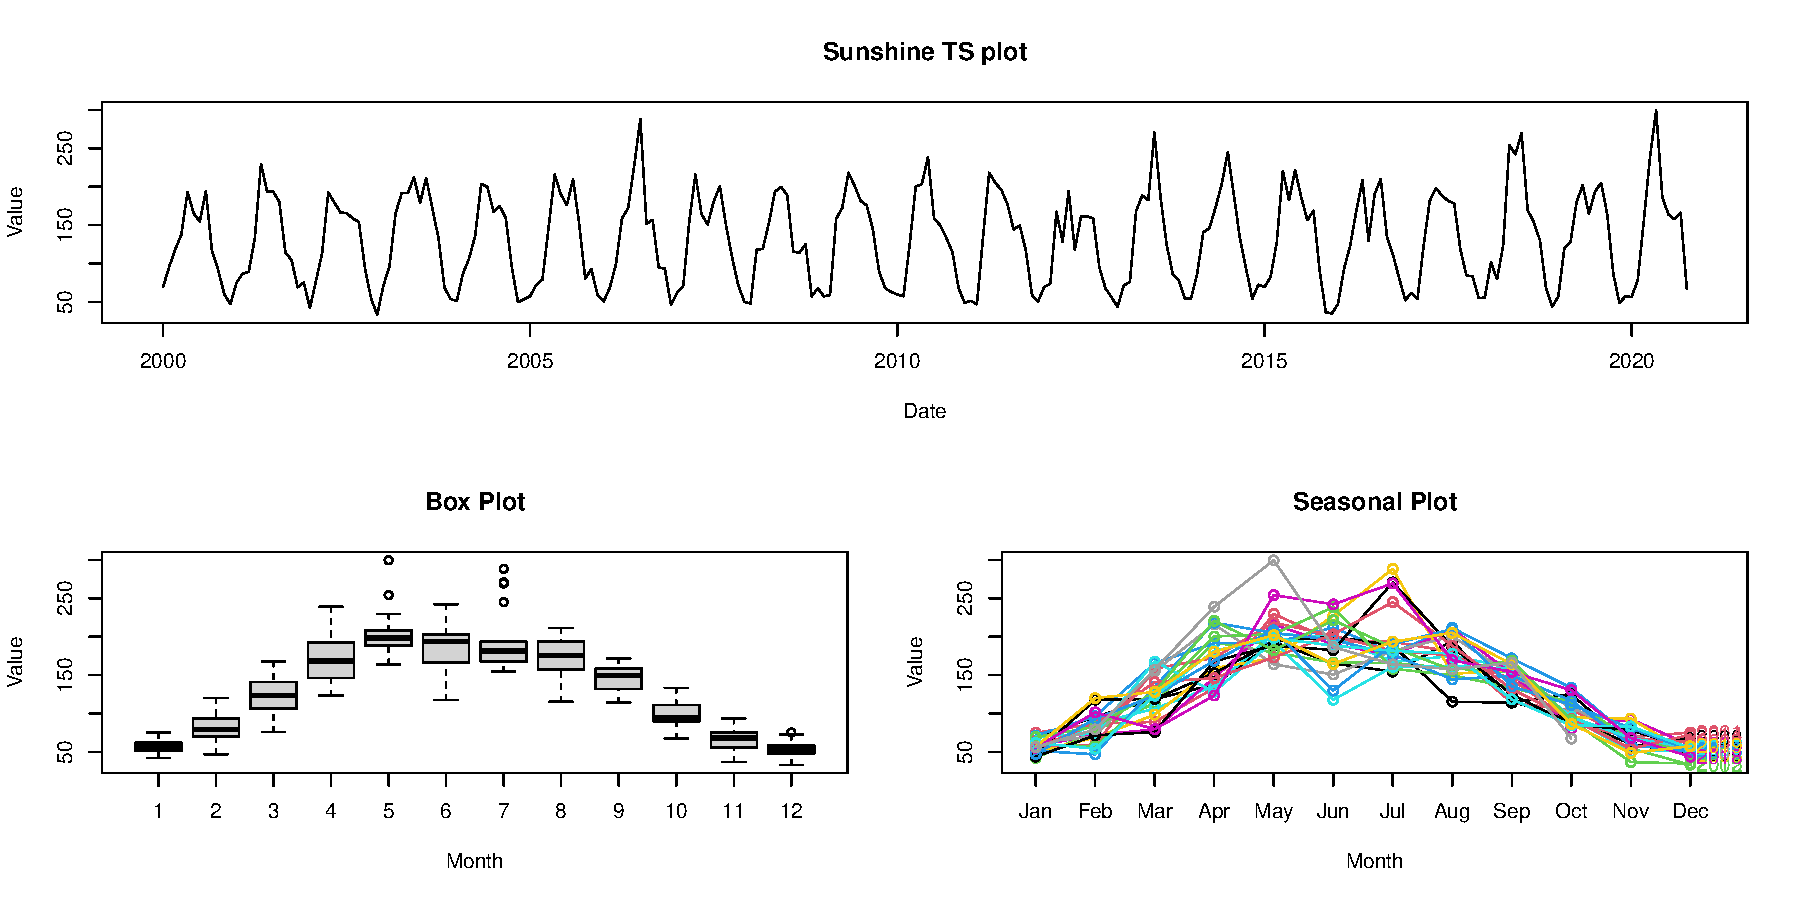
\includegraphics{ST422_files/figure-latex/unnamed-chunk-6-1.pdf}
\caption{Preliminary analysis on trimmed Sunshine series}
\end{figure}

\begin{figure}
\centering
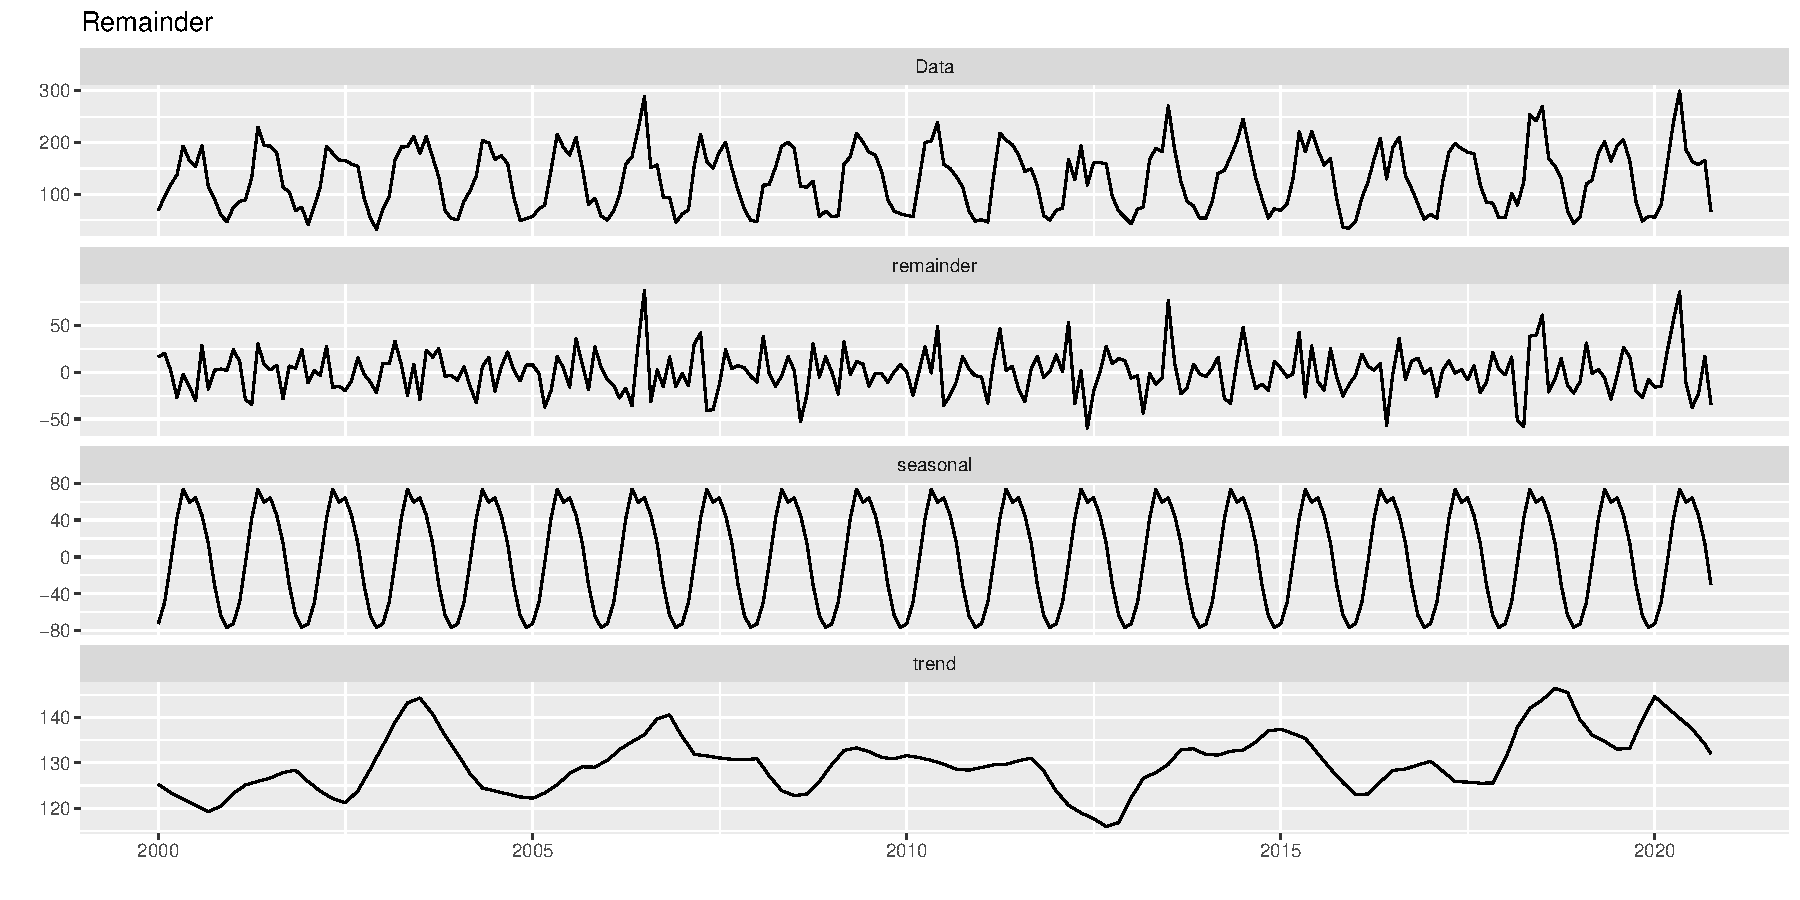
\includegraphics{ST422_files/figure-latex/unnamed-chunk-7-1.pdf}
\caption{Decomposition analysis on trimmed Sunshine series}
\end{figure}

\newpage

Based on preliminary analysis plots on \textbf{Sunshine} series,
following observations are made:

\begin{enumerate}
\def\labelenumi{\arabic{enumi}.}
\tightlist
\item
  Monthly time-series plot shows high fluctuation but no visible trend
  nor increasing variance.
\item
  Box plots and seasonal plot indicate a definite existence of
  seasonality.
\item
  Decomposition analysis provide some additional insights that the trend
  cycle and the seasonal plot shows there's seasonal fluctuation
  occurred with no specific trend and fairly random remainder/residual.
\end{enumerate}

Conducted analysis indicates that sunshine peaks during summer (around
July) and reaches the lowest point during winter (around Dec). Which is
a common climate condition in countries with 4 distinct seasons
(e.g.~UK, Korea and Japan).

Given this observed seasonality in time series, I further delve into the
existence of seasonal persistence and the time series model
identification with ACF \& PACF plots.

\newpage

\hypertarget{acf-pacf-and-stationarity-analysis}{%
\subsubsection{ACF, PACF and stationarity
analysis}\label{acf-pacf-and-stationarity-analysis}}

\begin{figure}
\centering
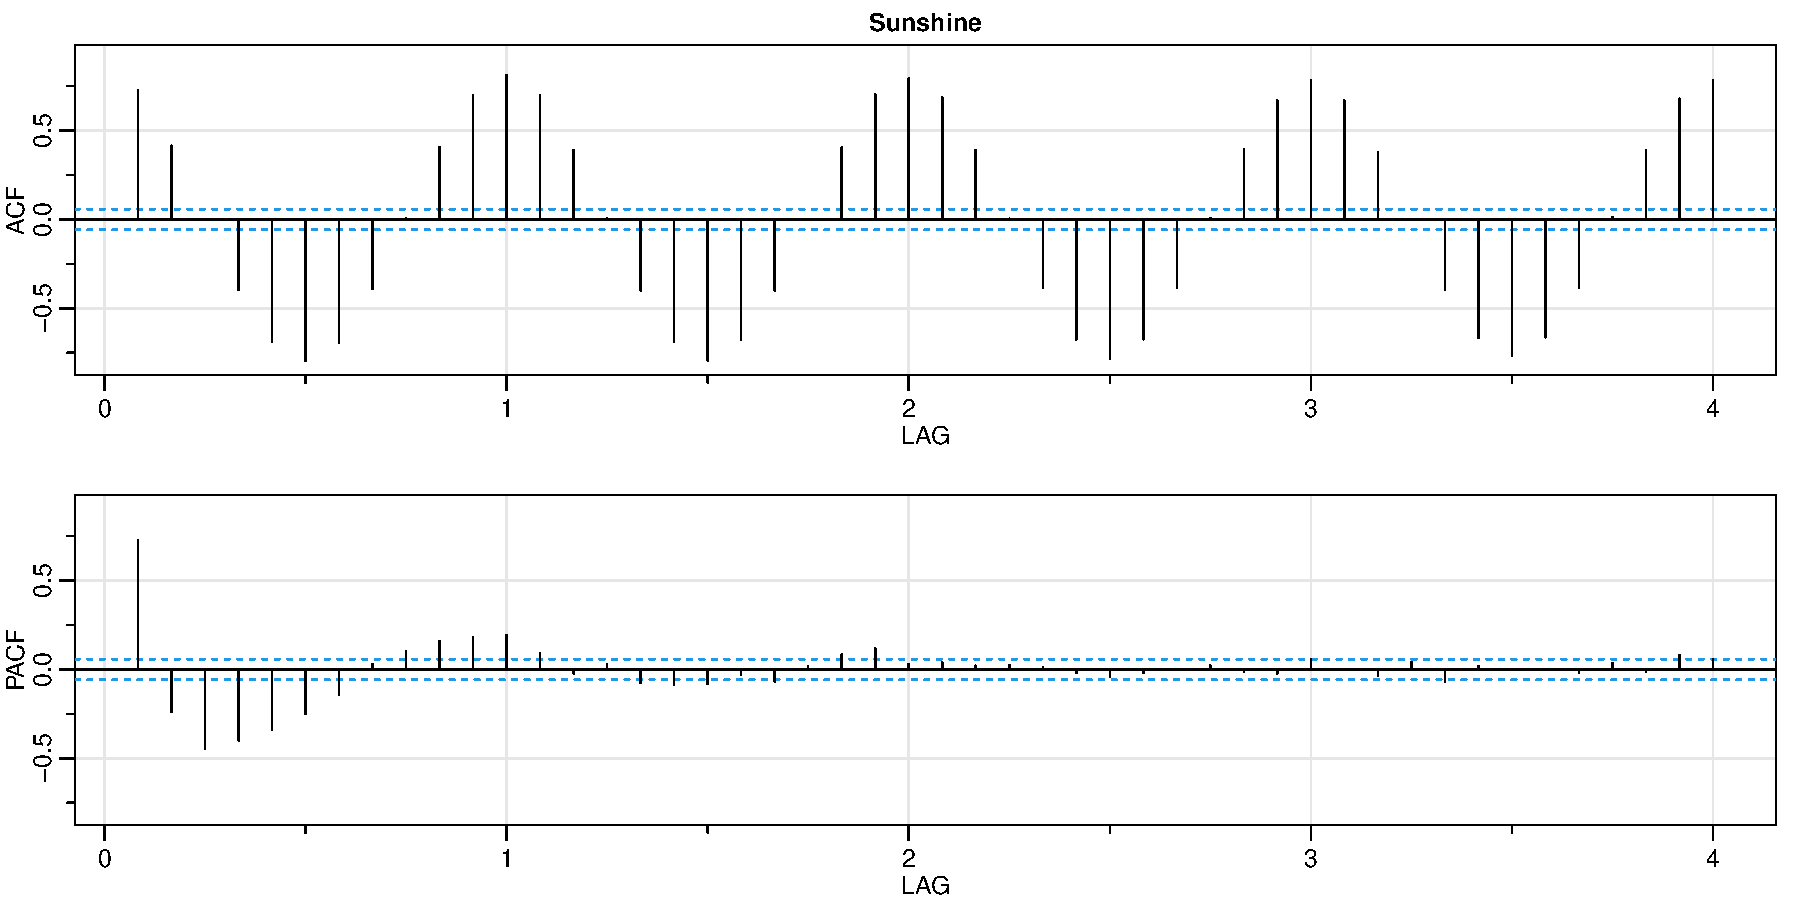
\includegraphics{ST422_files/figure-latex/unnamed-chunk-9-1.pdf}
\caption{ACF \& PACF plots of Sunshine series}
\end{figure}

\begin{verbatim}
## 
##  Augmented Dickey-Fuller Test
## 
## data:  ts_v
## Dickey-Fuller = -7.1097, Lag order = 12, p-value = 0.01
## alternative hypothesis: stationary
\end{verbatim}

Prior to ACF and PACF assessment, there is one of the most important
conditions required for time-series analysis that I need to check,
stationarity. Augmented Dickey-Fuller test is the most commonly used
test method to attest the stationarity of series. Based on the conducted
analysis, I could reject the null hypothesis at 5\% significance level
that the series is stationary.

In addition, based on ACF and PACF plots of Sunshine series, I can
verify the existence of seasonal persistence around 12 every month and
can gain further insights and draw the blueprint of our model
specification (Figure 5):

\begin{enumerate}
\def\labelenumi{\arabic{enumi}.}
\tightlist
\item
  ACF cuts off at lag 2 and PACF tails off -\textgreater{} MA(2)
\item
  Other model suggestion \& exploration with modifying AR and MA
  component by \(\pm1\)
\end{enumerate}

Based on seasonal pattern observed in the preliminary analysis,
consideration of a multiplicative seasonal ARIMA model is reasonable.
our variable of interest, monthly sunshine \(x_t\) as being modeled as:

\[x_t = S_t + w_t\]

where \(S_t\) is a seasonal component that varies a little from one year
to the next.

As a next step, 12 month differencing is going to be examined to find a
roughly stationary series and then find a multiplicative seasonal ARIMA
to fit the resulting residual series.

\newpage

\hypertarget{nabla_12-series-analysis}{%
\subsubsection{\texorpdfstring{\(\nabla_{12}\) series
analysis}{\textbackslash nabla\_\{12\} series analysis}}\label{nabla_12-series-analysis}}

\begin{figure}
\centering
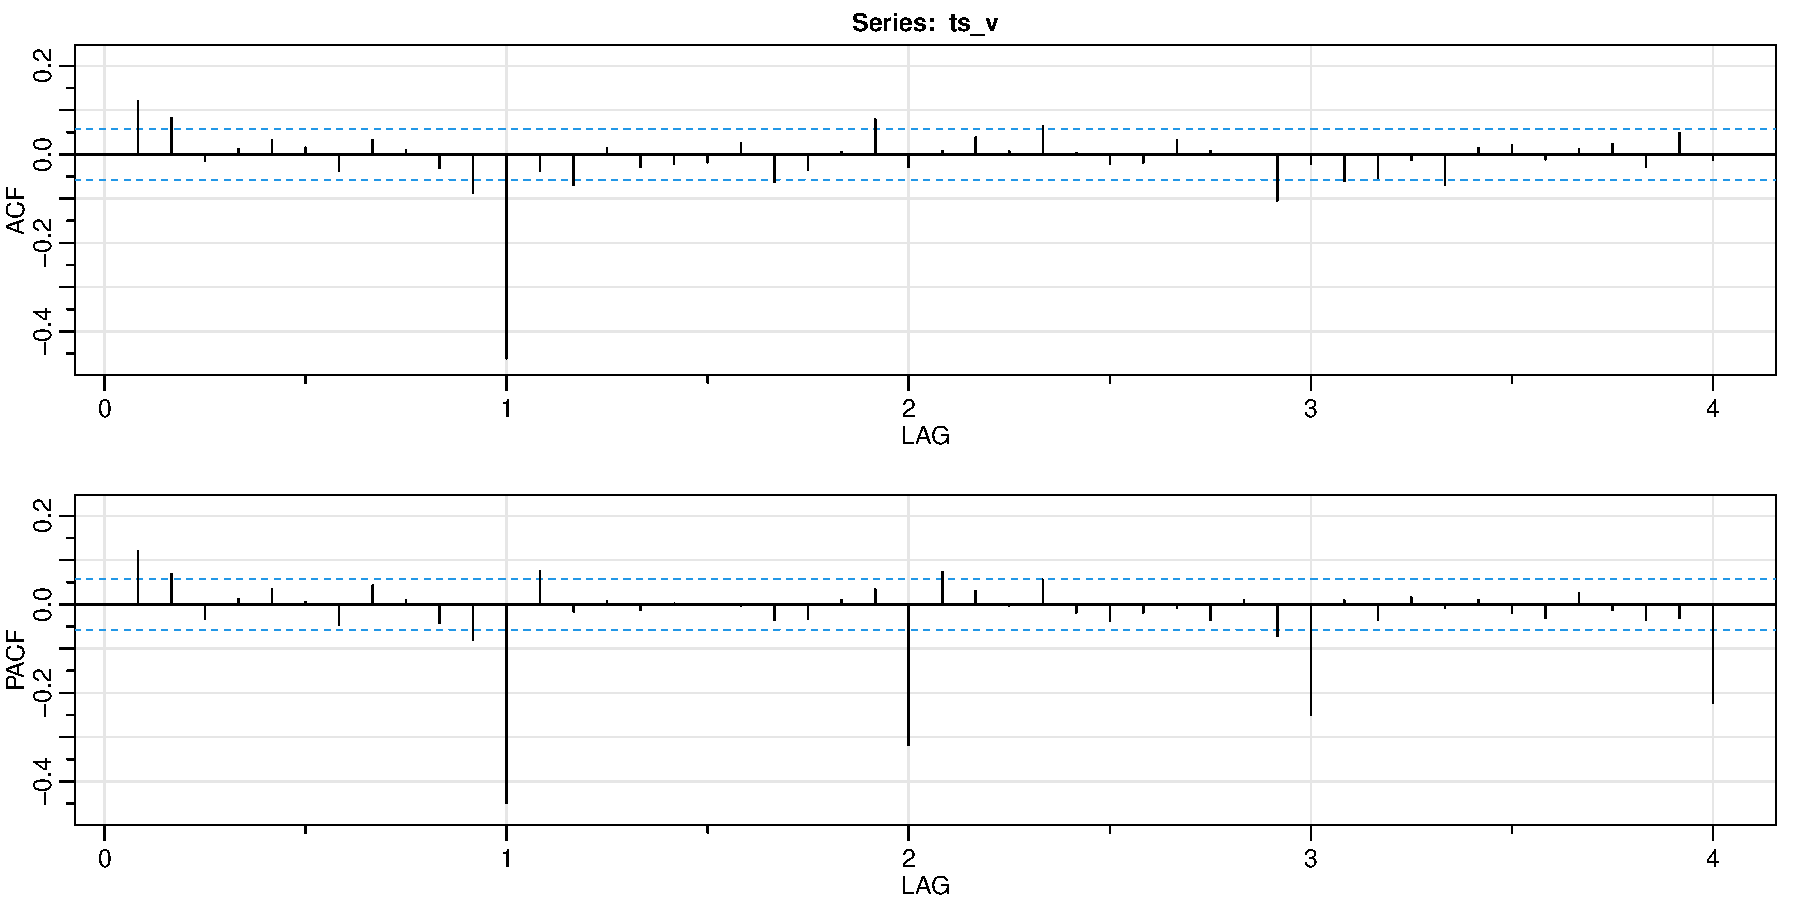
\includegraphics{ST422_files/figure-latex/unnamed-chunk-10-1.pdf}
\caption{ACF \& PACF plots of seasonally differenced Sunshine series}
\end{figure}

\begin{verbatim}
## 
##  Augmented Dickey-Fuller Test
## 
## data:  ts_v
## Dickey-Fuller = -14.374, Lag order = 12, p-value = 0.01
## alternative hypothesis: stationary
\end{verbatim}

The resulting ACF and PACF possibly indicate that (Figure 6):

\begin{enumerate}
\def\labelenumi{\arabic{enumi}.}
\tightlist
\item
  ACF cuts off at lag 1 and PACF decays quickly -\textgreater{} MA(1)
\item
  Other model suggestion \& exploration with modifying AR and MA
  component by \(\pm1\)
\end{enumerate}

\newpage

\hypertarget{model-fitting-using-sarima}{%
\subsubsection{Model fitting using
SARIMA}\label{model-fitting-using-sarima}}

In this section, I fit the optimal parameters of the time-series model
based on insights gained from previous analysis and extend the scope
with other models based on the suggestion with modifying AR and MA
component by \(\pm1\). For model exploration, the exhaustive approach
(i.e.~grid-search) will be used to calculate the goodness of fit of a
possible set models and rank them based on the performance (i.e.~AIC).
Furthermore, an additional candidate model using auto.arima() function
from the third party R package is going to be examined as well. Hence,
total 3 different specifications will be compared:

\begin{enumerate}
\def\labelenumi{\arabic{enumi}.}
\tightlist
\item
  \(ARMA(0,0,2)\times(0,1,1)_{12}\) \textless- Best guess model based on
  preliminary analysis.
\item
  Grid-search model
\item
  auto.arima() model
\end{enumerate}

Initial non-seasonal \& seasonal parameters for grid-search approach are
derived from Model 1: \(ARMA(0,0,2)\times(0,1,1)_{12}\).

\newpage

\hypertarget{model-diagnosis-and-final-model-selection}{%
\subsubsection{Model diagnosis and final model
selection}\label{model-diagnosis-and-final-model-selection}}

\begin{verbatim}
## Series: ss_ts 
## ARIMA(0,0,2)(0,1,1)[12] 
## 
## Coefficients:
##          ma1     ma2     sma1
##       0.1315  0.0627  -0.9533
## s.e.  0.0288  0.0282   0.0107
## 
## sigma^2 estimated as 661.5:  log likelihood=-5658.96
## AIC=11325.91   AICc=11325.95   BIC=11346.31
\end{verbatim}

\begin{verbatim}
## Series: ss_ts 
## ARIMA(0,0,2)(0,1,1)[12] 
## 
## Coefficients:
##          ma1     ma2     sma1
##       0.1315  0.0627  -0.9533
## s.e.  0.0288  0.0282   0.0107
## 
## sigma^2 estimated as 661.5:  log likelihood=-5658.96
## AIC=11325.91   AICc=11325.95   BIC=11346.31
\end{verbatim}

\begin{verbatim}
## Series: ss_ts 
## ARIMA(0,0,2)(2,1,0)[12] 
## 
## Coefficients:
##          ma1     ma2     sar1     sar2
##       0.1410  0.0839  -0.6171  -0.3370
## s.e.  0.0289  0.0284   0.0273   0.0277
## 
## sigma^2 estimated as 868.5:  log likelihood=-5811.72
## AIC=11633.43   AICc=11633.48   BIC=11658.93
\end{verbatim}

Resulted 3 different models can be found below:

\begin{enumerate}
\def\labelenumi{\arabic{enumi}.}
\tightlist
\item
  \(ARMA(0,0,2)\times(0,1,1)_{12}\) \textless- Model(1) Best guess
\item
  \(ARMA(0,0,2)\times(0,1,1)_{12}\) \textless- Model(2) Grid-search
\item
  \(ARMA(0,0,2)\times(2,1,0)_{12}\) \textless- Model(3) auto.arima
\end{enumerate}

Based on the goodness of fit metrics (i.e.~AIC) of 3 different models,
Model(1) and Model(2) are identical and provide better model-fit results
compared to Model(3). Hence, the final model is:
\(ARMA(1,0,0)\times(0,1,1)_{12}\).

\begin{Shaded}
\begin{Highlighting}[]
\CommentTok{# Residual analysis}
\KeywordTok{checkresiduals}\NormalTok{(best_guess_ss)}
\end{Highlighting}
\end{Shaded}

\begin{figure}
\centering
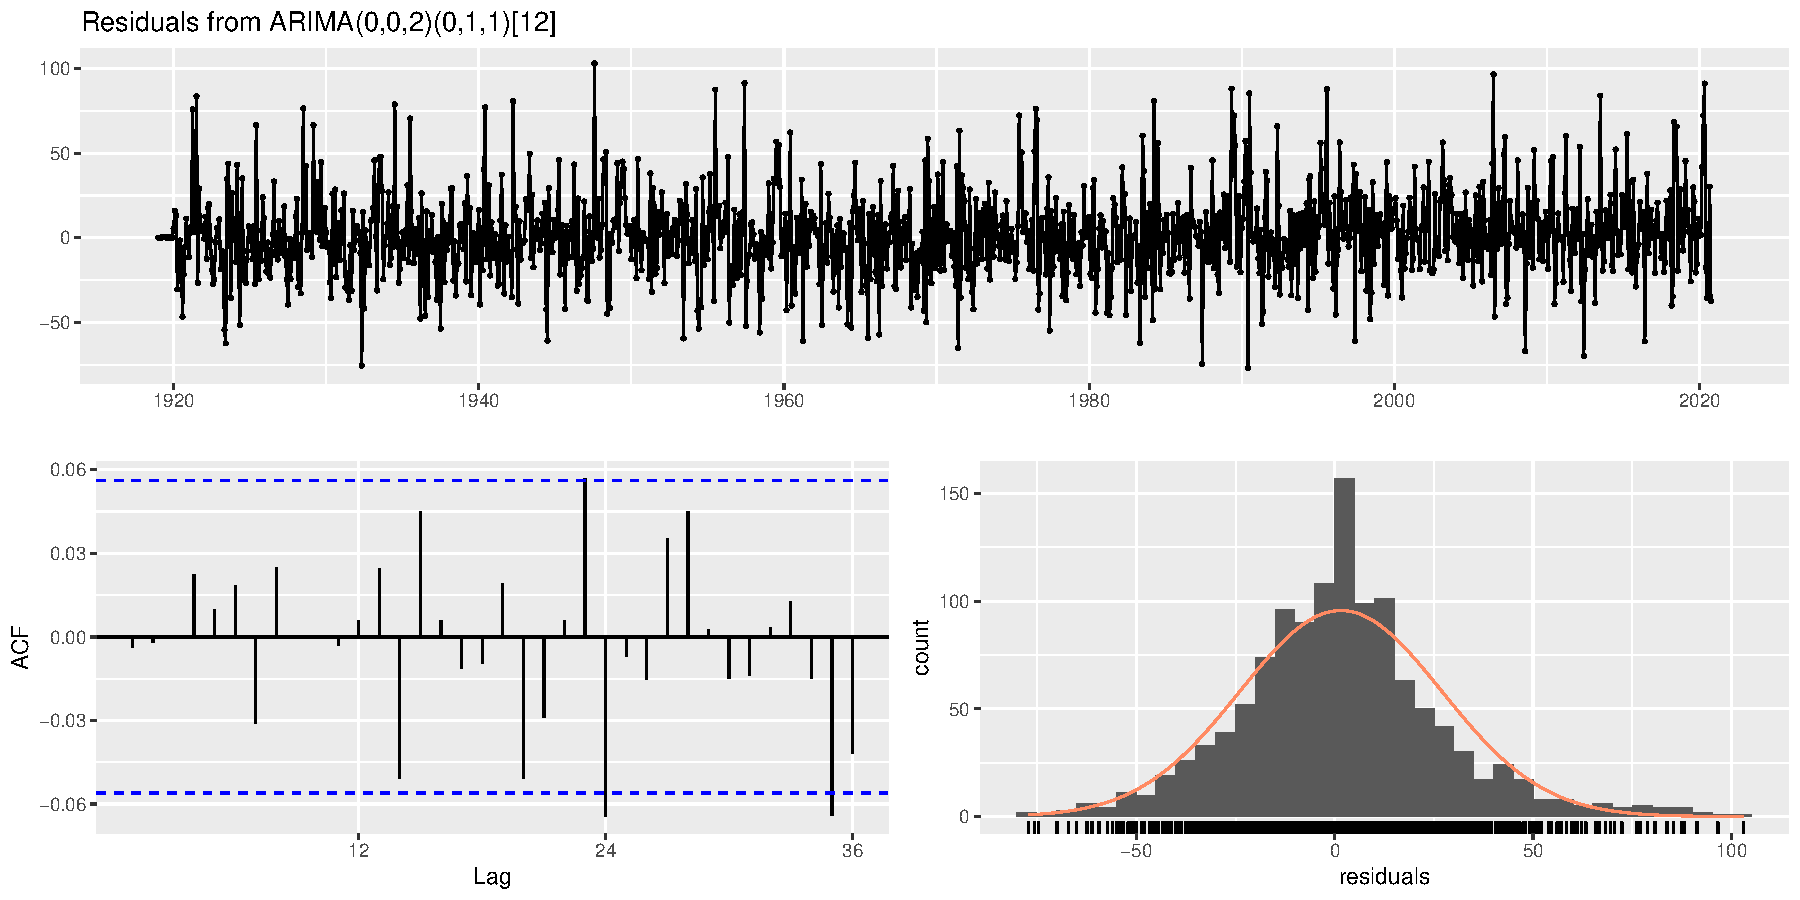
\includegraphics{ST422_files/figure-latex/unnamed-chunk-14-1.pdf}
\caption{Residual diagnosis}
\end{figure}

\begin{verbatim}
## 
##  Ljung-Box test
## 
## data:  Residuals from ARIMA(0,0,2)(0,1,1)[12]
## Q* = 23.931, df = 21, p-value = 0.2964
## 
## Model df: 3.   Total lags used: 24
\end{verbatim}

\begin{Shaded}
\begin{Highlighting}[]
\KeywordTok{tsdiag}\NormalTok{(best_guess_ss)}
\end{Highlighting}
\end{Shaded}

\begin{figure}
\centering
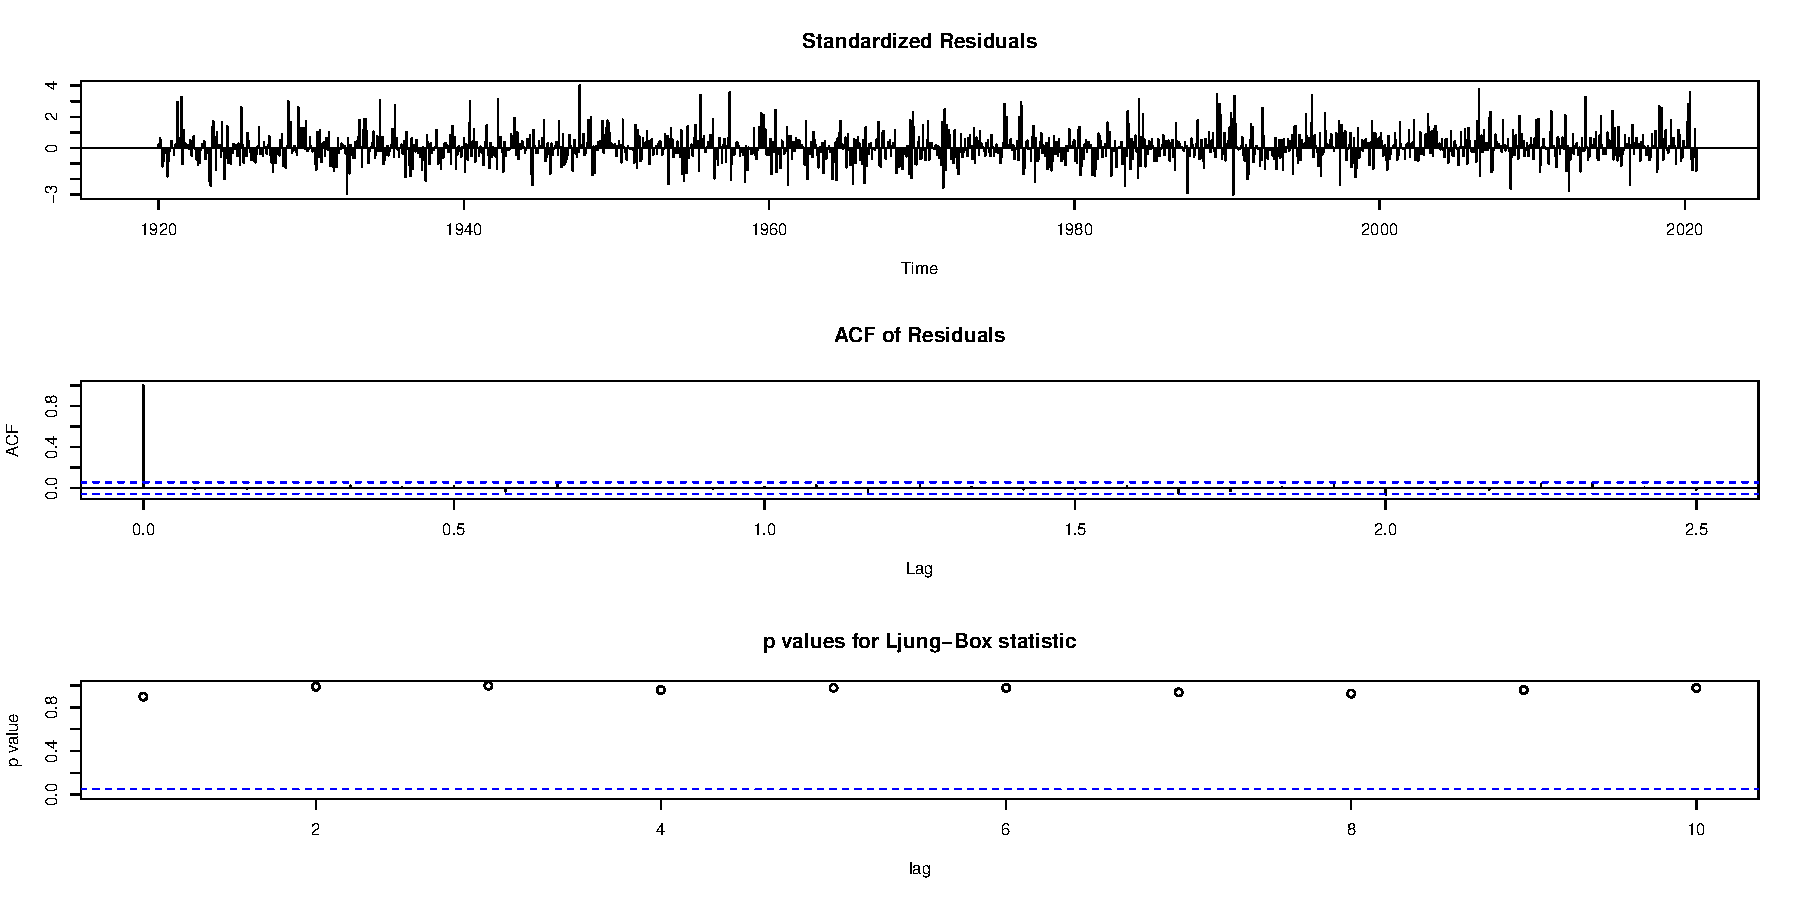
\includegraphics{ST422_files/figure-latex/unnamed-chunk-14-2.pdf}
\caption{Residual diagnosis}
\end{figure}

\newpage

Based on Figure (7) \& (8), the Ljung-Box test show no autocorrelation
on residuals and no seasonality observed on the ACF plot of model
residuals. Hence, it is concluded that the final model is appropriate
for forecasting since its residuals show white noise behavior and
uncorrelated against each other. As a next step, the forecasting of the
final model is going to be examined.

\newpage

\hypertarget{model-forecasting}{%
\subsubsection{Model forecasting}\label{model-forecasting}}

As a finale, I plot 2 months forecasting plot (Figure 9) and 24 months
(Figure 10) forecast plot to inspect the behaviour of estimated values.

\begin{figure}
\centering
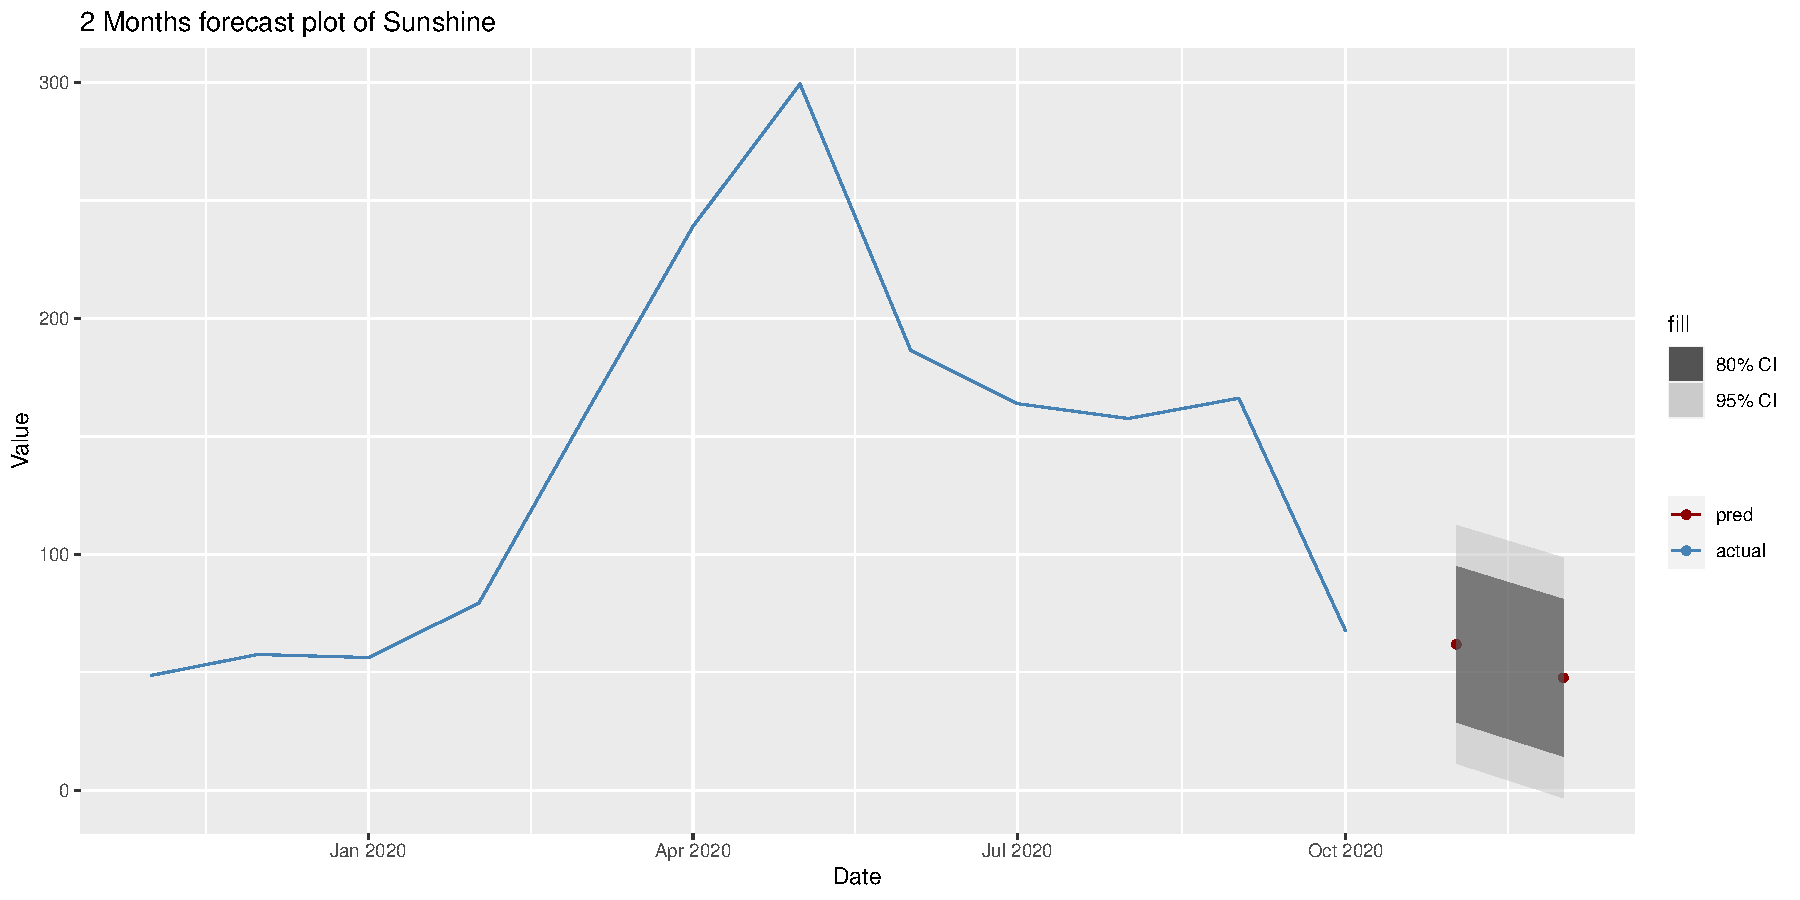
\includegraphics{ST422_files/figure-latex/unnamed-chunk-16-1.pdf}
\caption{2 Month forecasting}
\end{figure}

\begin{verbatim}
##          Point Forecast    Lo 80    Hi 80     Lo 95     Hi 95
## Nov 2020       61.89698 28.93614 94.85783 11.487717 112.30625
## Dec 2020       47.69690 14.45247 80.94134 -3.146075  98.53988
\end{verbatim}

Based on forecast visual plots, I can conclude that the final model is
following a general trend without any observed outlines.

\begin{figure}
\centering
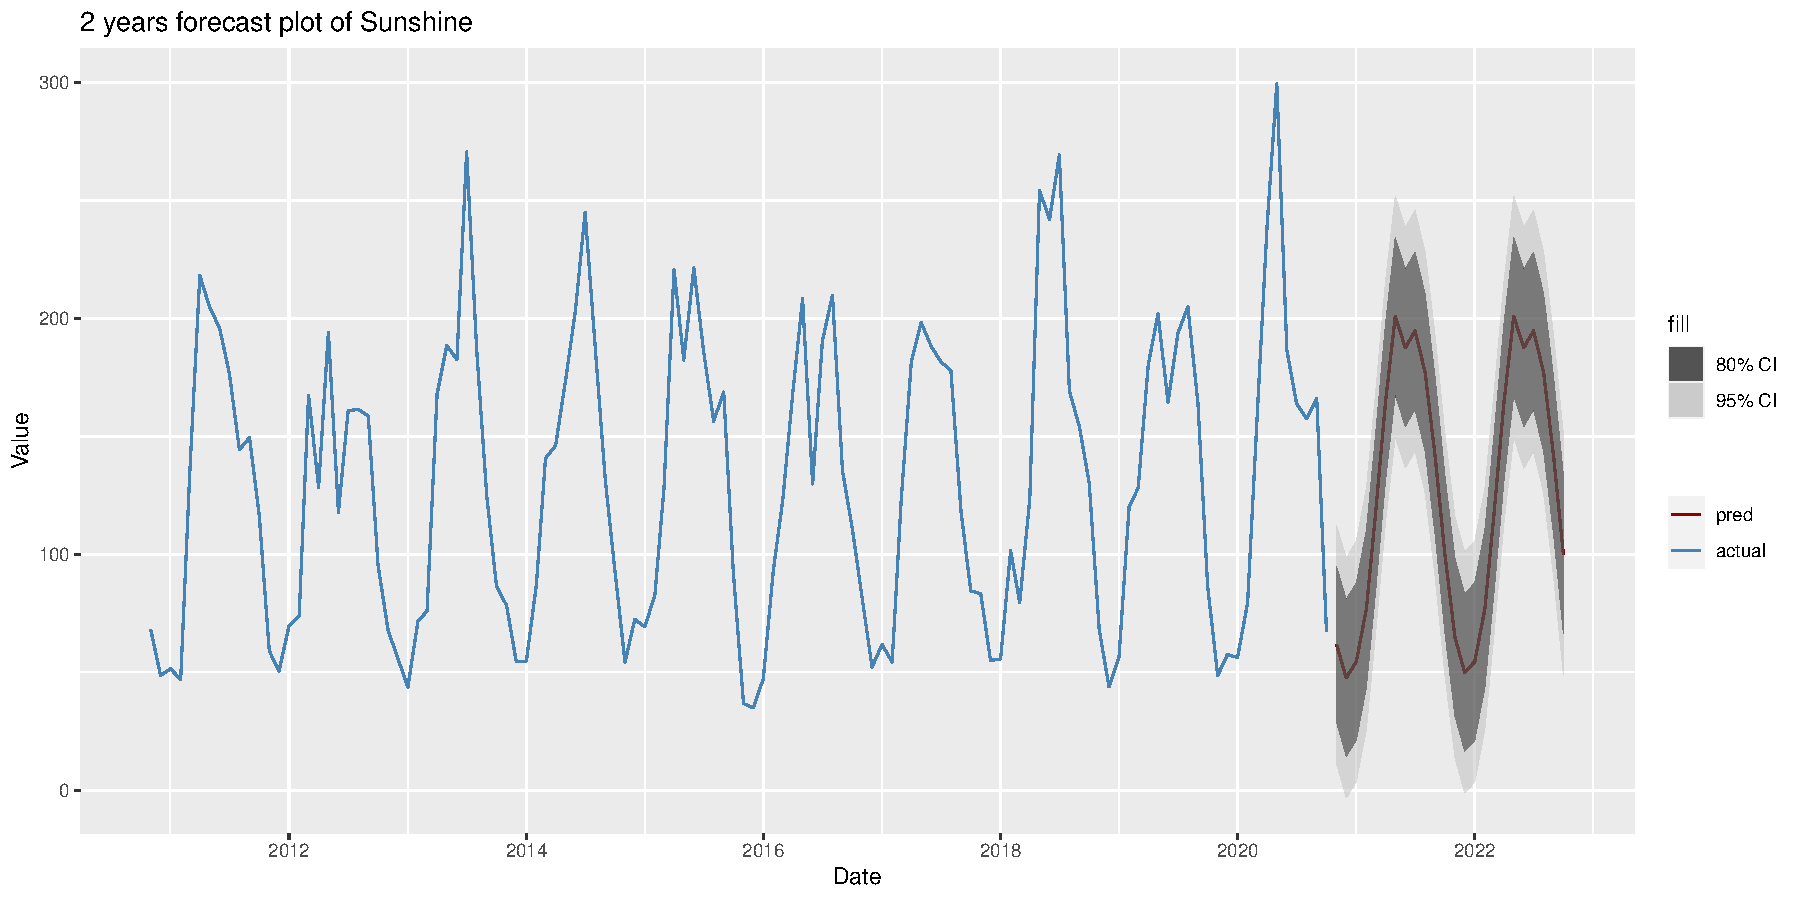
\includegraphics{ST422_files/figure-latex/unnamed-chunk-17-1.pdf}
\caption{24 Month forecasting}
\end{figure}

\newpage
\newpage
\newpage

\hypertarget{rainfall-series}{%
\subsection{Rainfall series}\label{rainfall-series}}

\hypertarget{preliminary-analysis-1}{%
\subsubsection{Preliminary analysis}\label{preliminary-analysis-1}}

\begin{figure}
\centering
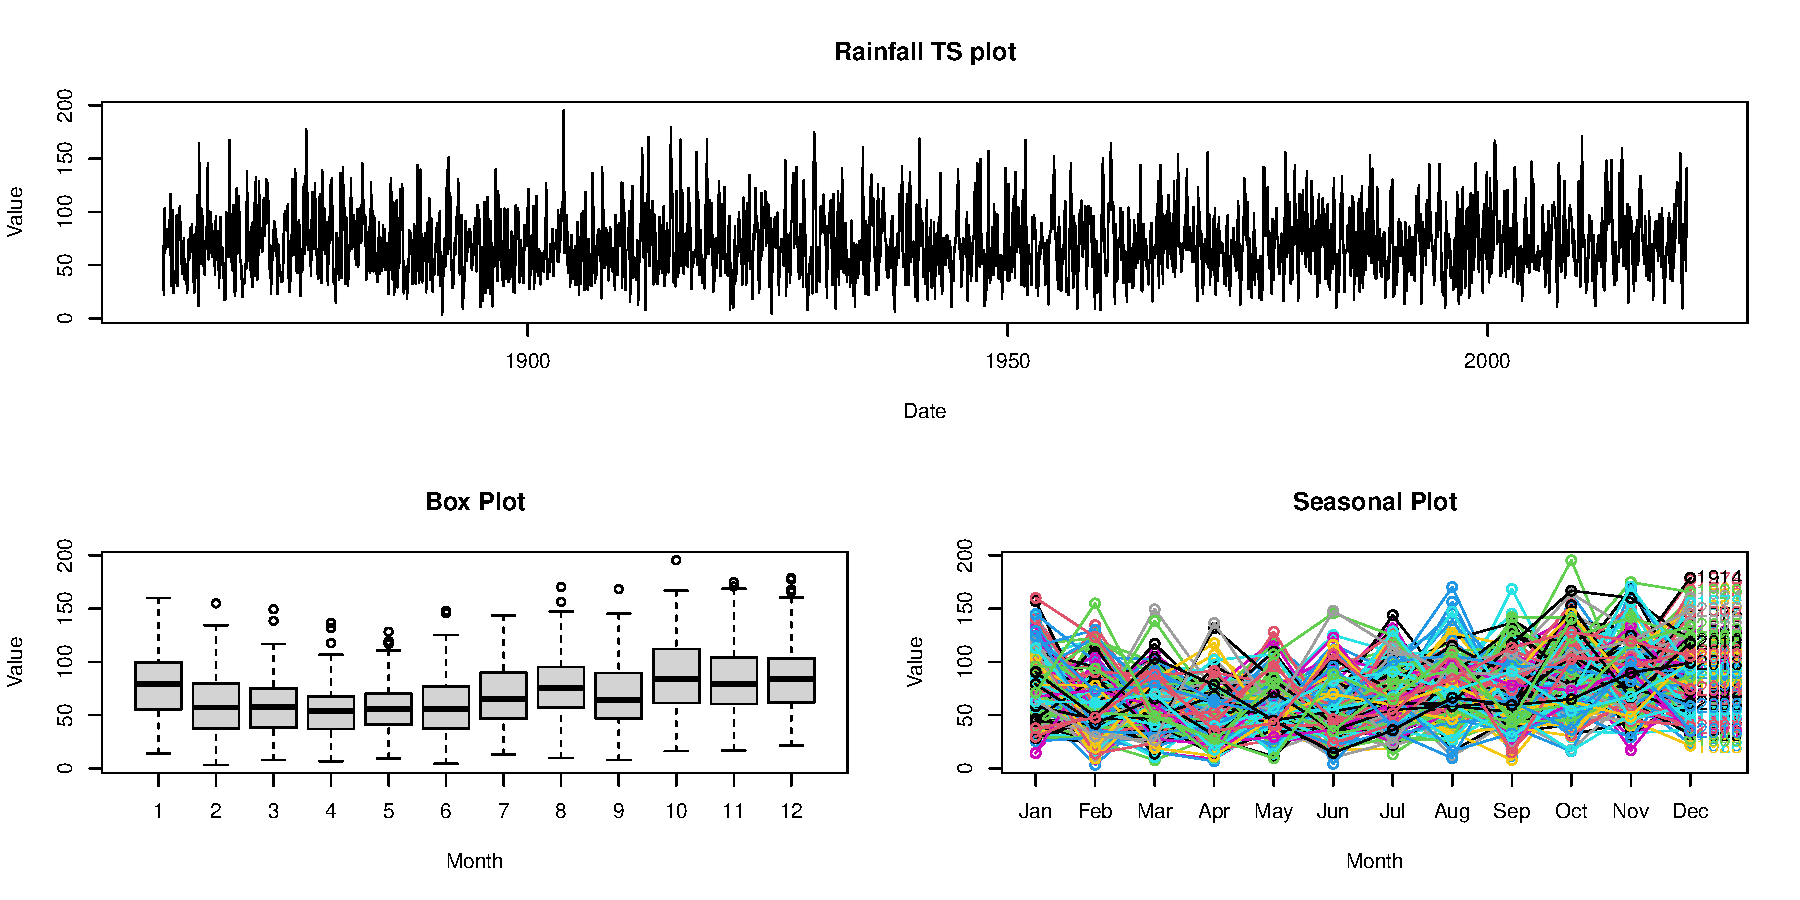
\includegraphics{ST422_files/figure-latex/unnamed-chunk-18-1.pdf}
\caption{Preliminary analysis on entire Rainfall series}
\end{figure}

\begin{figure}
\centering
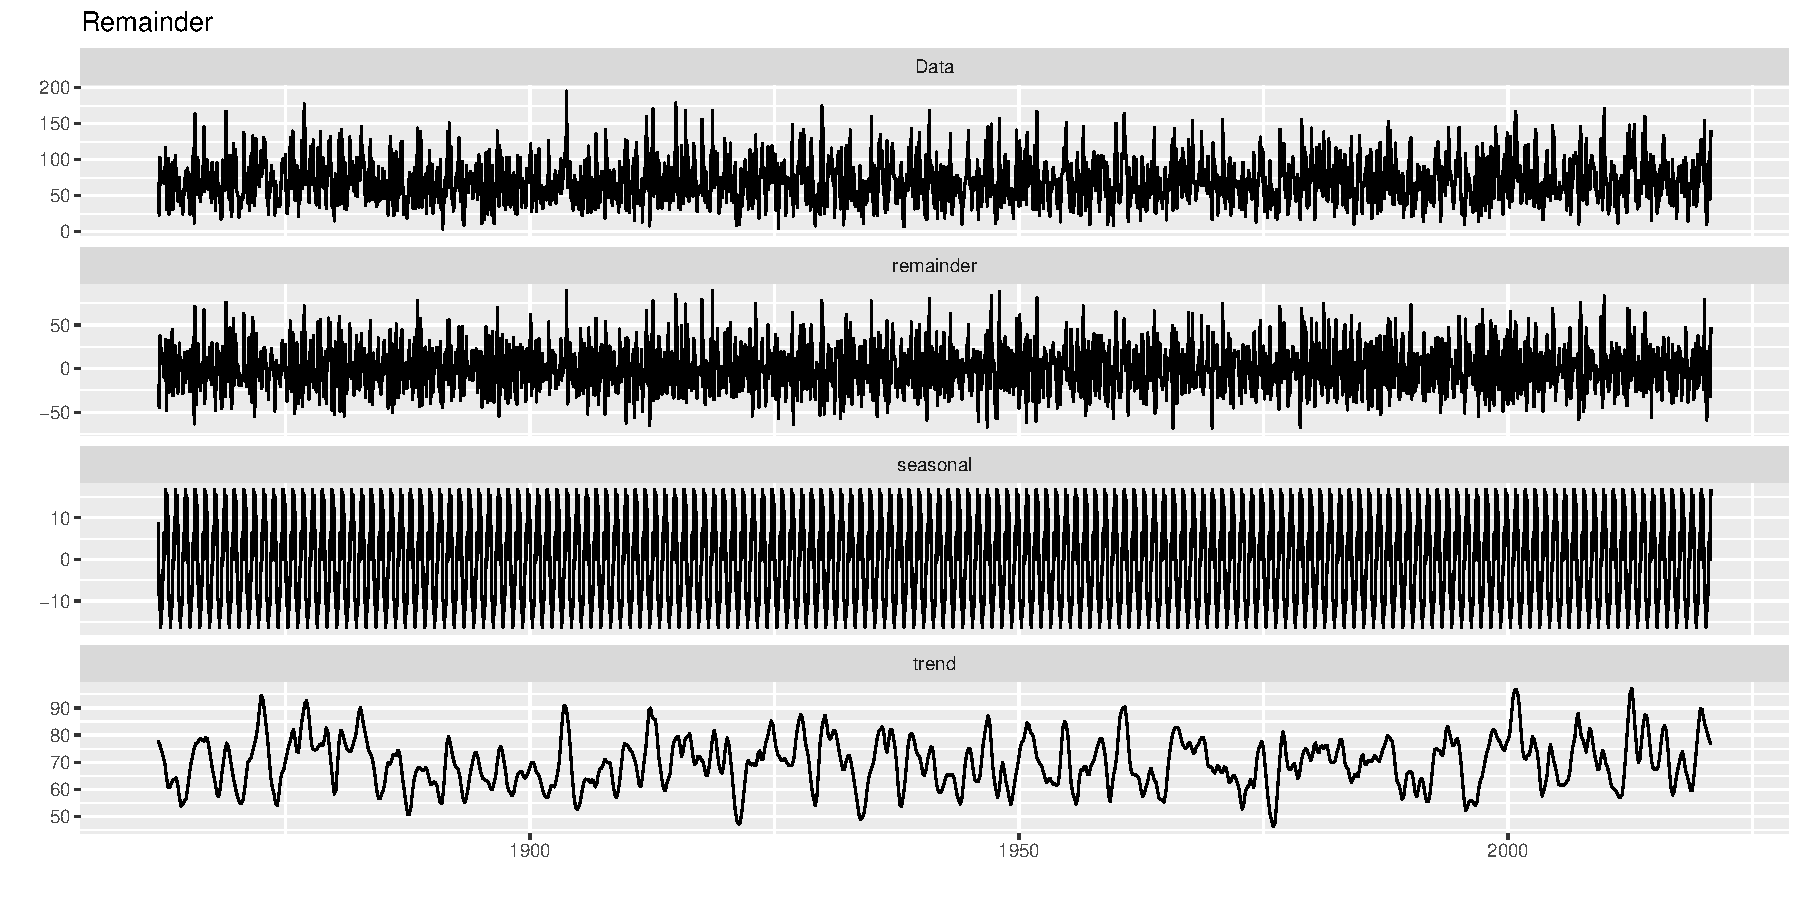
\includegraphics{ST422_files/figure-latex/unnamed-chunk-19-1.pdf}
\caption{Decomposition analysis on entire Rainfall series}
\end{figure}

By comparing the preliminary analysis based on the entire dataset
(Figure 11) and partial dataset (Figure 13), using the entire dataset is
a bit of stretch and there is no major difference in terms of the unique
patterns and trends observed between these two datasets. Hence, for
better intuitive understanding on analysis, the preliminary analysis is
conducted on the partial dataset (21st century) but the final modelling
will be using the entire population.

\newpage

\begin{figure}
\centering
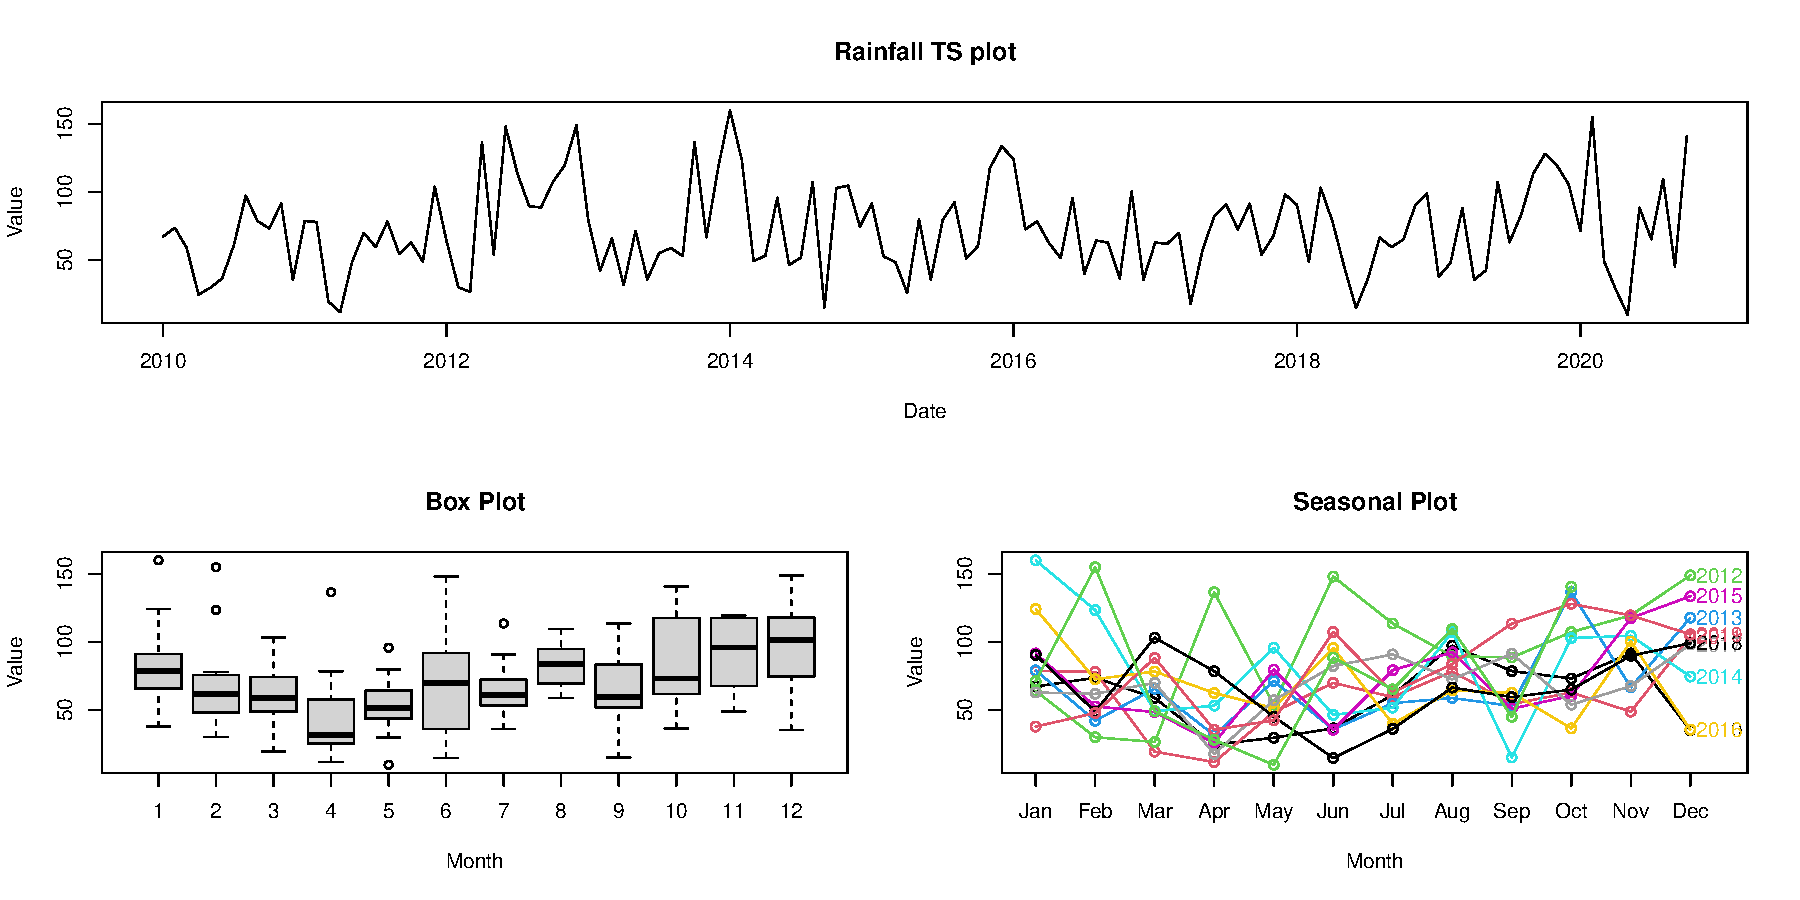
\includegraphics{ST422_files/figure-latex/unnamed-chunk-20-1.pdf}
\caption{Preliminary analysis on trimmed Rainfall series}
\end{figure}

\begin{figure}
\centering
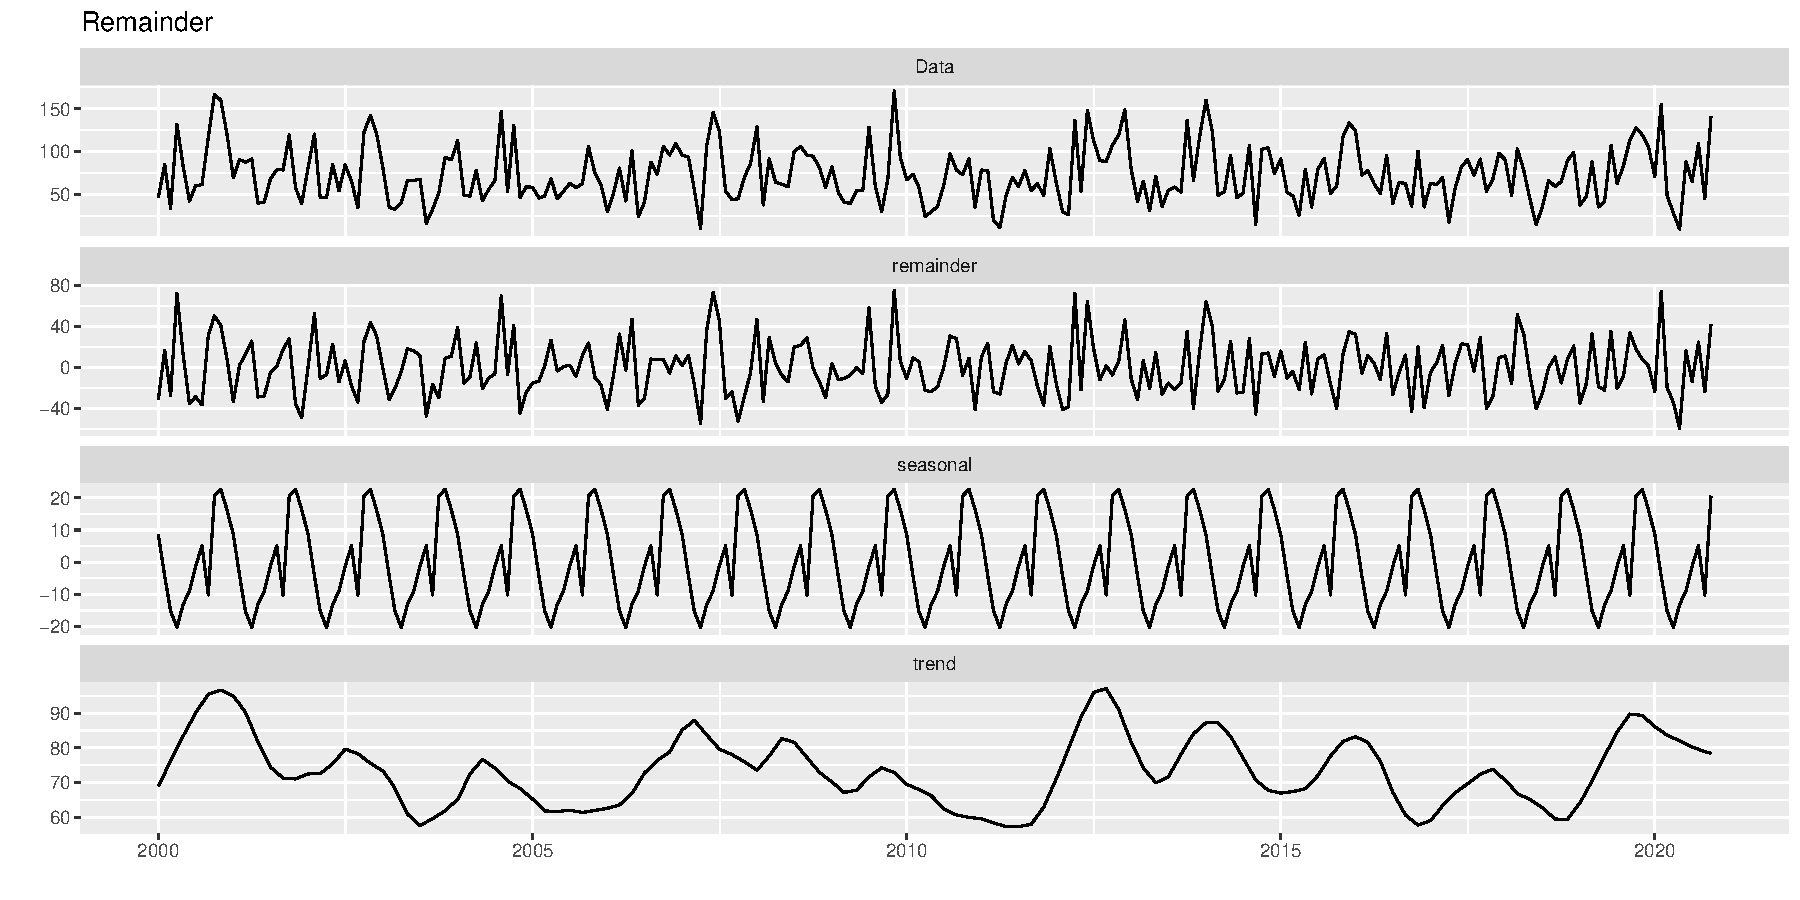
\includegraphics{ST422_files/figure-latex/unnamed-chunk-21-1.pdf}
\caption{Decomposition analysis on trimmed Rainfall series}
\end{figure}

Based on preliminary analysis plots on \textbf{Rainfall} series,
following observations are made:

\begin{enumerate}
\def\labelenumi{\arabic{enumi}.}
\tightlist
\item
  Monthly time-series plot shows high fluctuation but no visible trend
  nor increasing variance.
\item
  Box plots and seasonal plot indicate the existence of seasonal trend.
\item
  Decomposition analysis provide some additional insights that the trend
  cycle and the seasonal plot shows there's seasonal fluctuation
  occurred with no specific trend and fairly random remainder/residual.
\end{enumerate}

Conducted analysis indicate that rainfall seems to be well dispersed
throughout the whole year. Notably, July and August are the wettest
months and late winter - spring (Feb \textasciitilde{} Mar) are the
driest months as well as autumn - winter (Oct \textasciitilde{} Jan) the
wettest.

Given this observed seasonality in time series, I further delve into the
existence of seasonal persistence and the time series model
identification with ACF \& PACF plots (Figure 15).

\newpage

\hypertarget{acf-pacf-and-stationarity-analysis-1}{%
\subsubsection{ACF, PACF and stationarity
analysis}\label{acf-pacf-and-stationarity-analysis-1}}

\begin{figure}
\centering
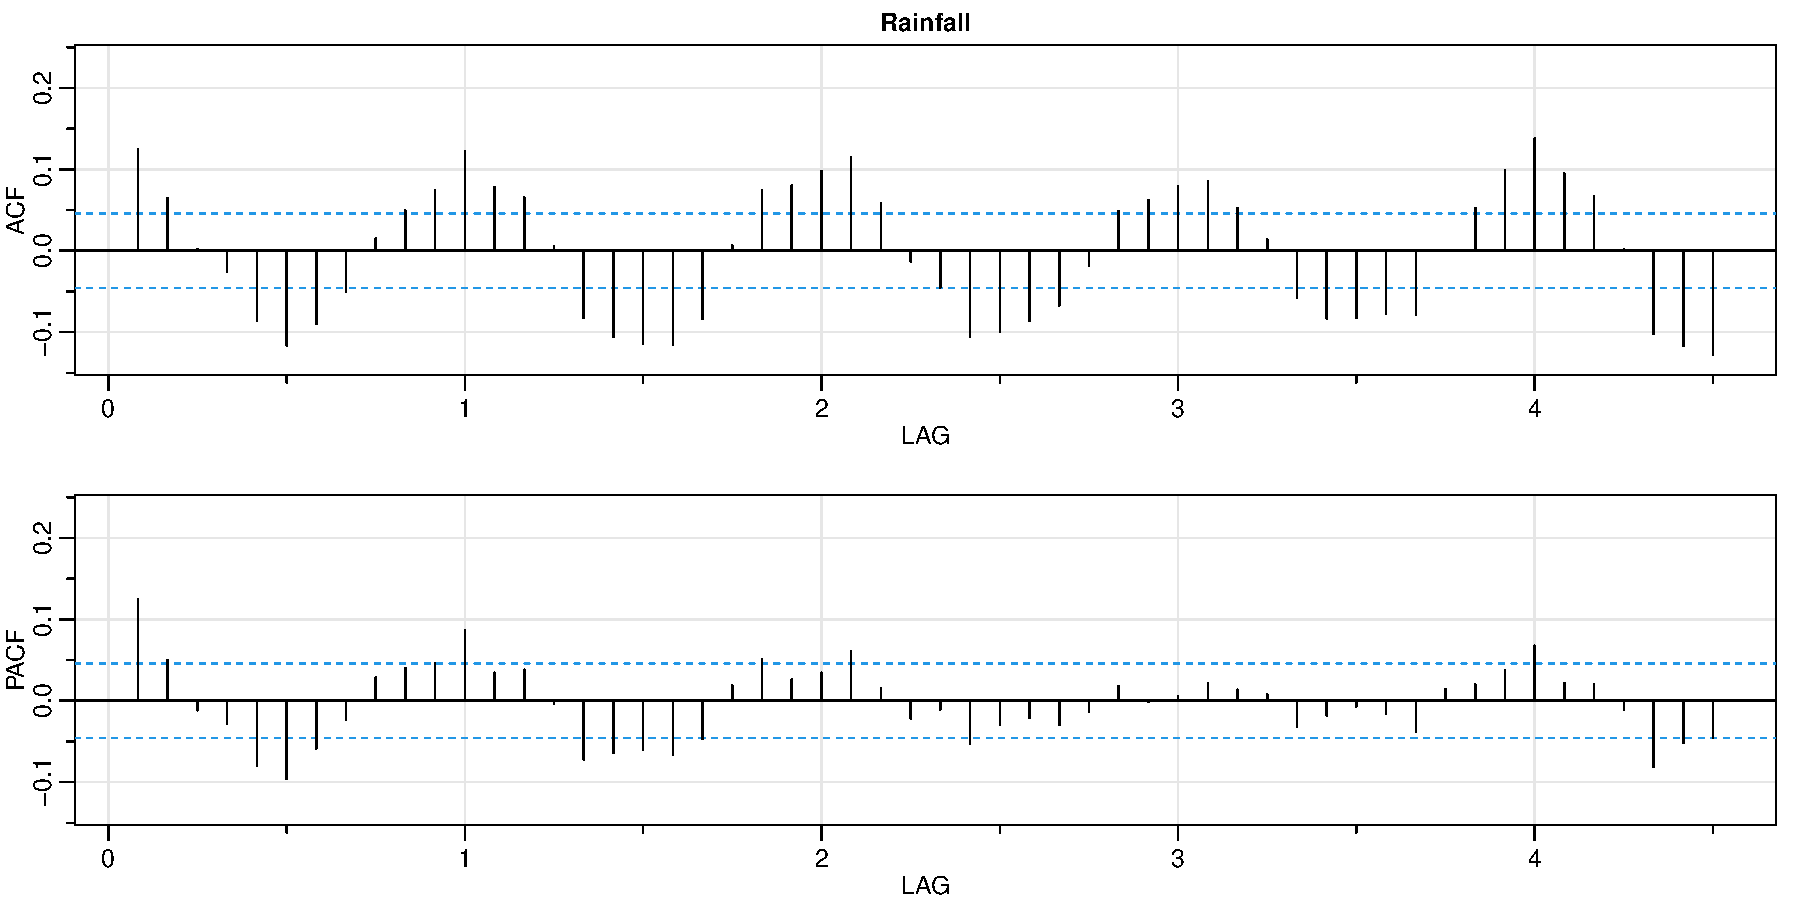
\includegraphics{ST422_files/figure-latex/unnamed-chunk-22-1.pdf}
\caption{ACF \& PACF plots of rainfall series}
\end{figure}

\begin{verbatim}
## 
##  Augmented Dickey-Fuller Test
## 
## data:  ts_v
## Dickey-Fuller = -10.874, Lag order = 12, p-value = 0.01
## alternative hypothesis: stationary
\end{verbatim}

Prior to ACF and PACF assessment, there is one of the most important
conditions required for time-series analysis that I need to check,
stationarity. Augmented Dickey-Fuller test is the most commonly used
test method to attest the stationarity of series. Based on the conducted
analysis, the result could reject the null hypothesis at 5\%
significance level that the series is stationary.

In addition, based on ACF and PACF plots, I can verify the existence of
seasonal persistence around 12 every month and can gain further insights
and draw the blueprint of our model specification:

\begin{enumerate}
\def\labelenumi{\arabic{enumi}.}
\tightlist
\item
  Both ACF and PACF tail off -\textgreater{} ARMA(1,1)
\item
  Other model suggestion \& exploration with modifying AR and MA
  component by \(\pm1\)
\end{enumerate}

Based on seasonal pattern observed in the preliminary analysis,
consideration of a multiplicative seasonal ARIMA model is reasonable.
Our variable of interest, monthly rainfall \(x_t\) as being modeled as:

\[x_t = S_t + w_t\]

where \(S_t\) is a seasonal component that varies a little from one year
to the next.

As a next step, 12 month differencing is going to be examined to find a
roughly stationary series and then find a multiplicative seasonal ARIMA
to fit the resulting residual series.

\newpage

\hypertarget{nabla_12-series-analysis-1}{%
\subsubsection{\texorpdfstring{\(\nabla_{12}\) series
analysis}{\textbackslash nabla\_\{12\} series analysis}}\label{nabla_12-series-analysis-1}}

\begin{figure}
\centering
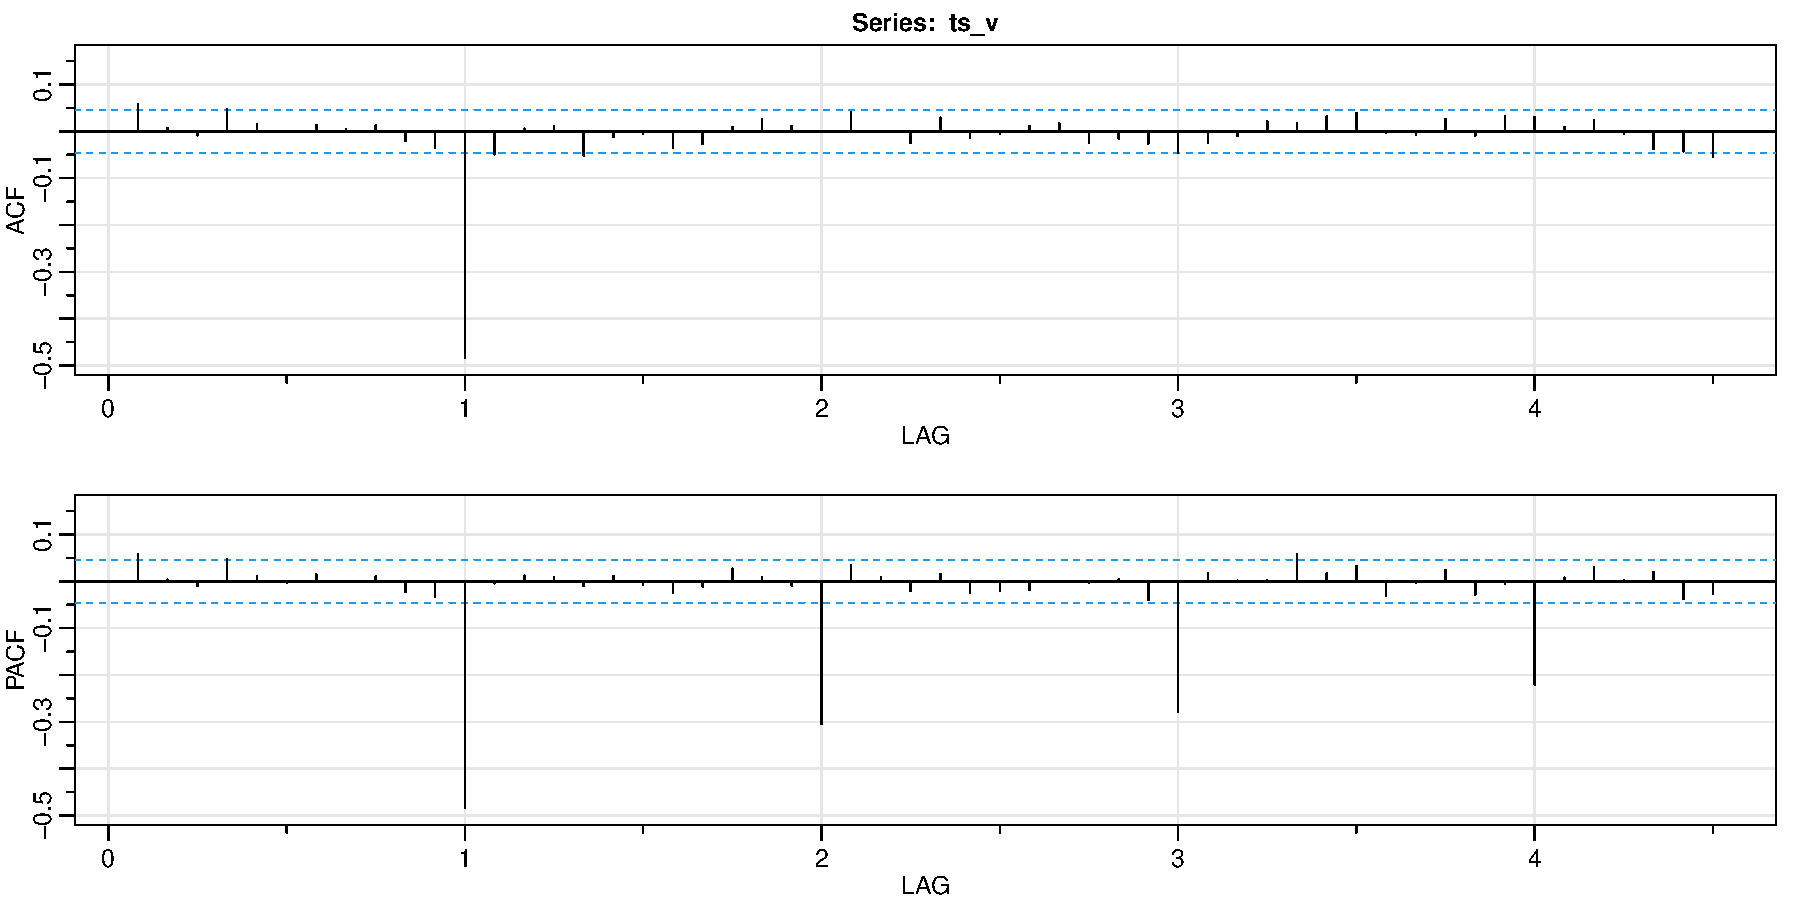
\includegraphics{ST422_files/figure-latex/unnamed-chunk-23-1.pdf}
\caption{ACF \& PACF plots of seasonally differenced rainfall series}
\end{figure}

\begin{verbatim}
## 
##  Augmented Dickey-Fuller Test
## 
## data:  ts_v
## Dickey-Fuller = -19.281, Lag order = 12, p-value = 0.01
## alternative hypothesis: stationary
\end{verbatim}

The resulting ACF and PACF (Figure 16) possibly indicate that:

\begin{enumerate}
\def\labelenumi{\arabic{enumi}.}
\tightlist
\item
  ACF cuts off at lag 1 and PACF decays quickly -\textgreater{} MA(1)
\item
  Other model suggestion \& exploration with modifying AR and MA
  component by \(\pm1\)
\end{enumerate}

\newpage

\hypertarget{model-fitting-using-sarima-1}{%
\subsubsection{Model fitting using
SARIMA}\label{model-fitting-using-sarima-1}}

In this section, I fit the optimal parameters of the time-series model
based on insights gained from previous analysis and extend the scope
with other models based on the suggestion with modifying AR and MA
component by \(\pm1\). For model exploration, an exhaustive approach
(i.e.~grid-search) will be used to calculate the goodness of fit of a
possible set models and rank them based on the performance (i.e.~AIC).
Furthermore, an additional candidate model using auto.arima() function
from the third party R package is going to be examined as well. Hence,
total 3 different specifications will be compared:

\begin{enumerate}
\def\labelenumi{\arabic{enumi}.}
\tightlist
\item
  \(ARMA(1,0,1)\times(0,1,1)_{12}\) \textless- Best guess model based on
  preliminary analysis.
\item
  Grid-search model
\item
  auto.arima() model
\end{enumerate}

Initial non-seasonal \& seasonal parameters for grid-search approach are
derived from Model 1: \(ARMA(1,0,1)\times(0,1,1)_{12}\).

\newpage

\hypertarget{model-diagnosis-and-final-model-selection-1}{%
\subsubsection{Model diagnosis and final model
selection}\label{model-diagnosis-and-final-model-selection-1}}

\begin{Shaded}
\begin{Highlighting}[]
\CommentTok{# Models}
\NormalTok{best_guess_rf }\CommentTok{# Best guess}
\end{Highlighting}
\end{Shaded}

\begin{verbatim}
## Series: rf_ts 
## ARIMA(1,0,1)(0,1,1)[12] 
## 
## Coefficients:
##          ar1      ma1     sma1
##       0.6180  -0.5841  -0.9952
## s.e.  0.4512   0.4617   0.0170
## 
## sigma^2 estimated as 908.2:  log likelihood=-9162.88
## AIC=18333.75   AICc=18333.77   BIC=18355.94
\end{verbatim}

\begin{Shaded}
\begin{Highlighting}[]
\NormalTok{optimal_rf }\CommentTok{# Grid-search}
\end{Highlighting}
\end{Shaded}

\begin{verbatim}
## Series: rf_ts 
## ARIMA(1,0,0)(0,1,1)[12] 
## 
## Coefficients:
##          ar1     sma1
##       0.0366  -0.9949
## s.e.  0.0230   0.0159
## 
## sigma^2 estimated as 908.4:  log likelihood=-9163.39
## AIC=18332.77   AICc=18332.78   BIC=18349.41
\end{verbatim}

\begin{Shaded}
\begin{Highlighting}[]
\NormalTok{auto_arima_rf }\CommentTok{# auto.arima}
\end{Highlighting}
\end{Shaded}

\begin{verbatim}
## Series: rf_ts 
## ARIMA(1,0,0)(2,0,0)[12] with non-zero mean 
## 
## Coefficients:
##          ar1    sar1    sar2     mean
##       0.1011  0.1031  0.0704  69.8524
## s.e.  0.0232  0.0231  0.0233   0.9733
## 
## sigma^2 estimated as 1003:  log likelihood=-9288.14
## AIC=18586.28   AICc=18586.31   BIC=18614.04
\end{verbatim}

Resulted 3 different models can be found below:

\begin{enumerate}
\def\labelenumi{\arabic{enumi}.}
\tightlist
\item
  \(ARMA(1,0,1)\times(0,1,1)_{12}\) \textless- Model(1) Best guess
\item
  \(ARMA(1,0,0)\times(0,1,1)_{12}\) \textless- Model(2) Grid-search
\item
  \(ARMA(1,0,0)\times(2,0,0)_{12}\) \textless- Model(3) auto.arima
\end{enumerate}

Based on the goodness of fit metrics of 3 different models, Model(1) and
Model(2) provided better model-fit results compared to Model(3). Even
though there is a marginal difference between Model(1) and Model(2),
given the fact that Model(1) shows insignificant coefficients, the final
model is narrowed down to Model(2): \(ARMA(1,0,0)\times(0,1,1)_{12}\).

\begin{figure}
\centering
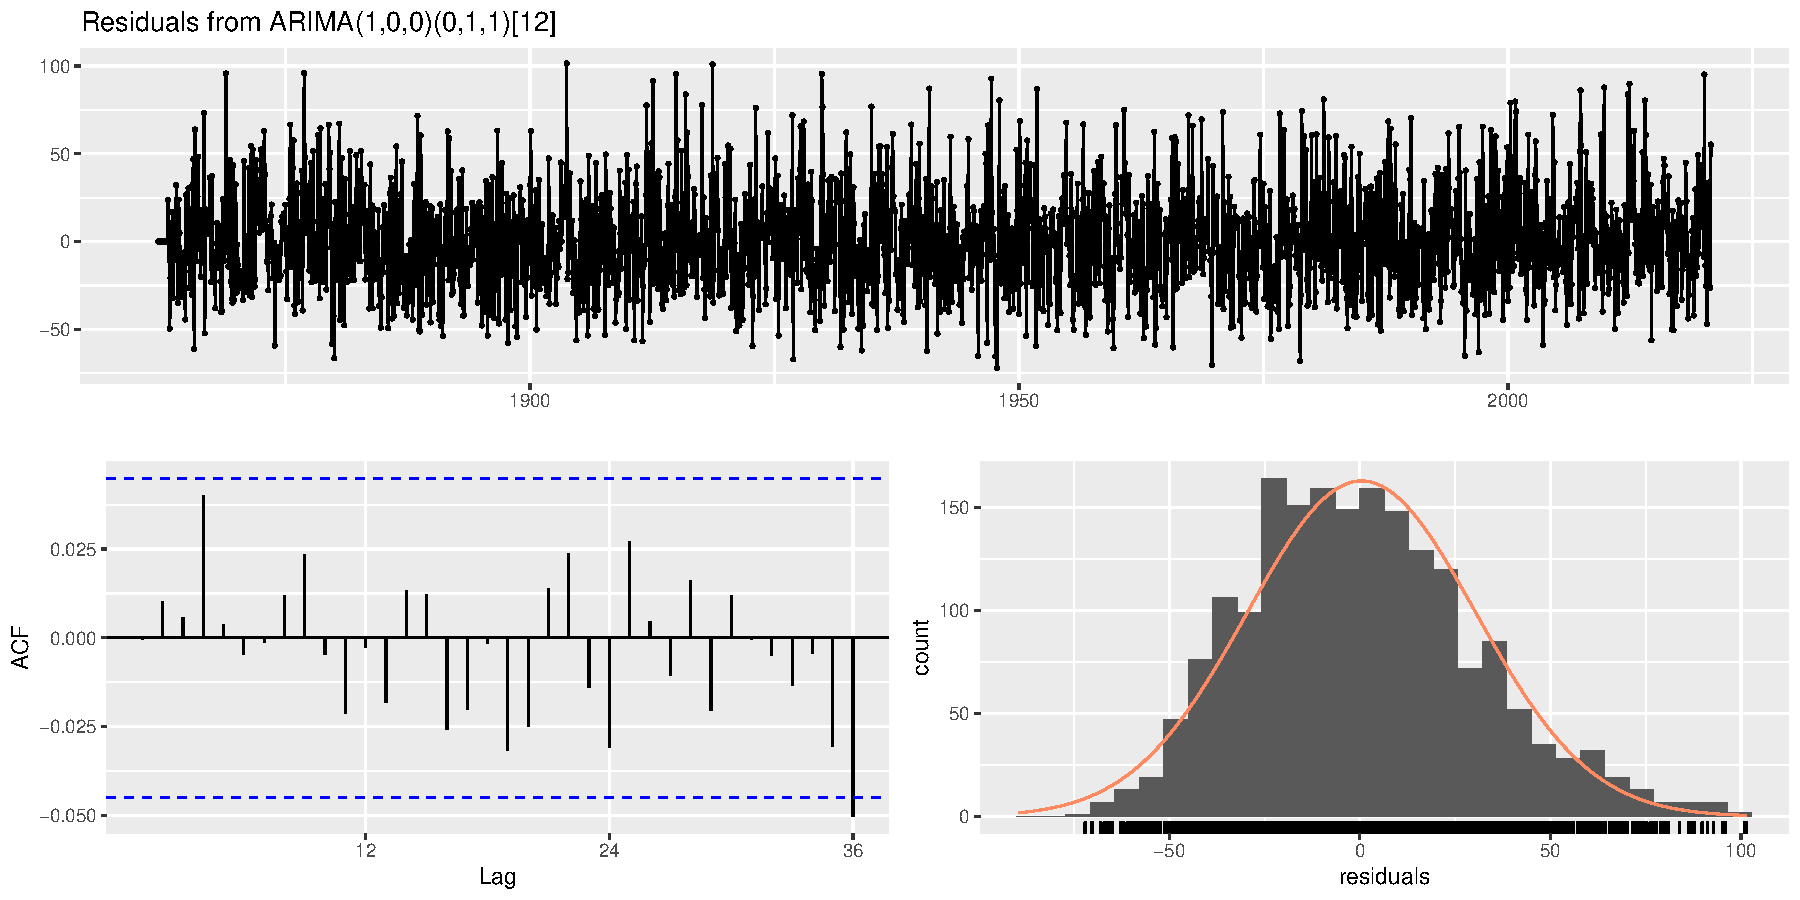
\includegraphics{ST422_files/figure-latex/unnamed-chunk-26-1.pdf}
\caption{Residual diagnosis}
\end{figure}

\begin{verbatim}
## 
##  Ljung-Box test
## 
## data:  Residuals from ARIMA(1,0,0)(0,1,1)[12]
## Q* = 15.809, df = 22, p-value = 0.8253
## 
## Model df: 2.   Total lags used: 24
\end{verbatim}

\begin{figure}
\centering
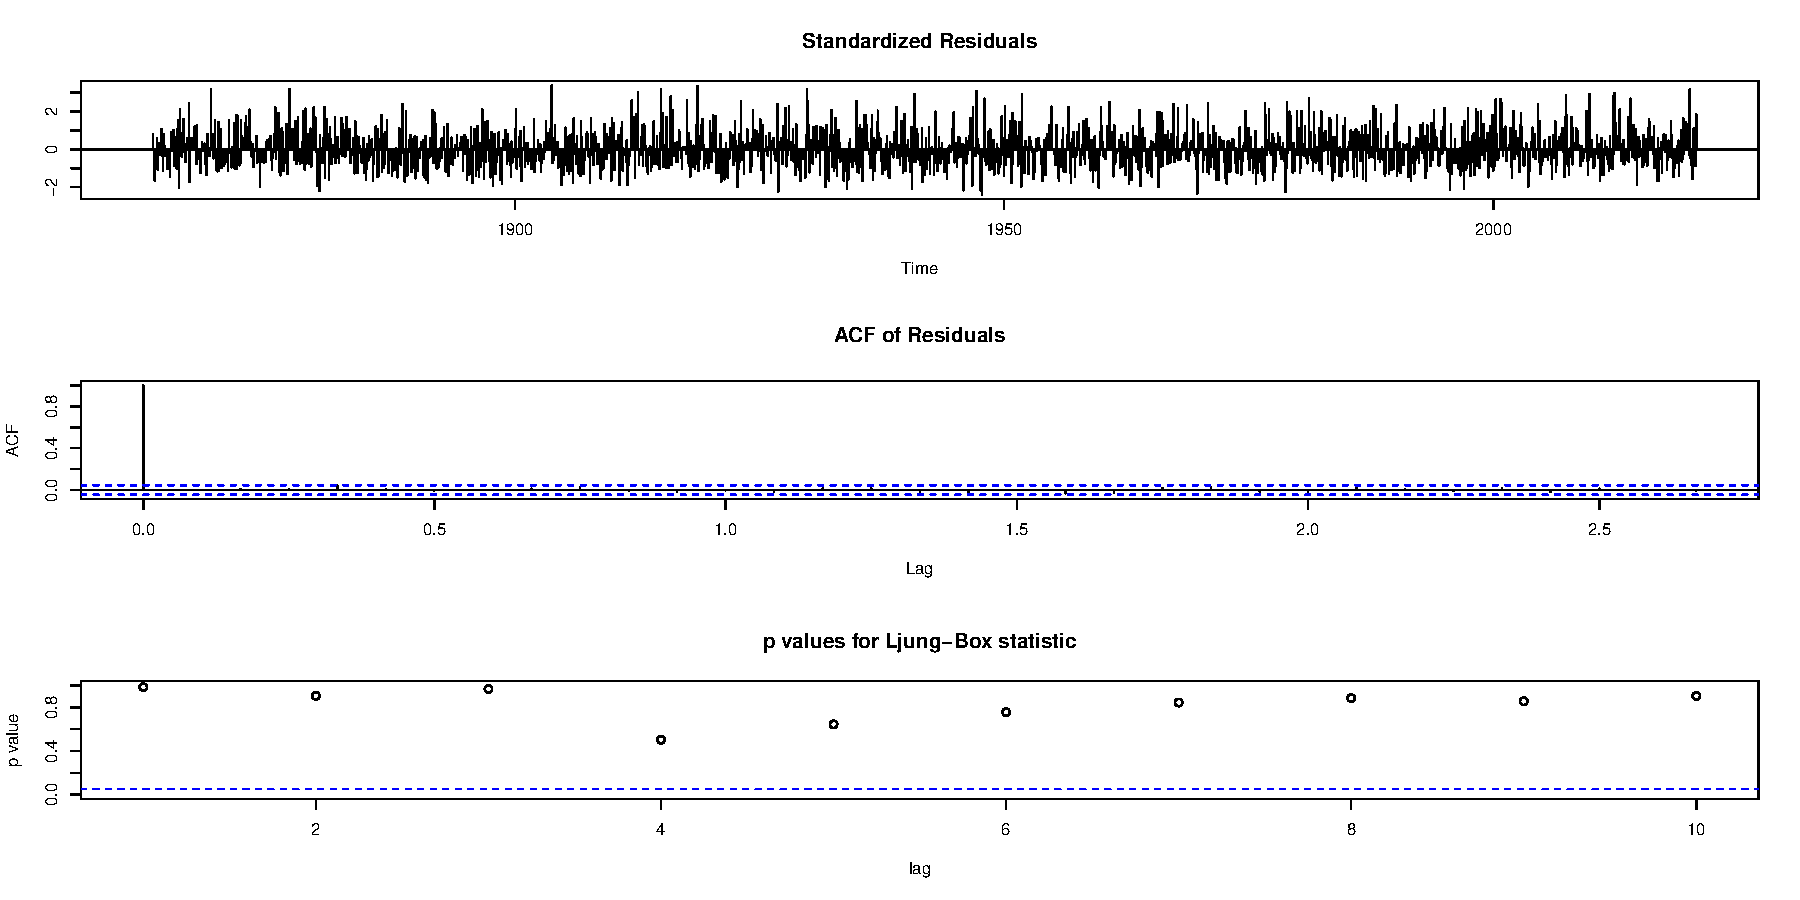
\includegraphics{ST422_files/figure-latex/unnamed-chunk-26-2.pdf}
\caption{Residual diagnosis}
\end{figure}

Based on the Ljung-Box test and ACF plot of model residuals (Figure 17,
18), it can be concluded that this model is appropriate for forecasting
since its residuals show white noise behavior and uncorrelated against
each other.

\newpage
\newpage

\hypertarget{model-forecasting-1}{%
\subsubsection{Model forecasting}\label{model-forecasting-1}}

As a finale, I plot 2 months forecasting plot and 24 months forecast
plot to inspect the behaviour of estimated values.

\begin{figure}
\centering
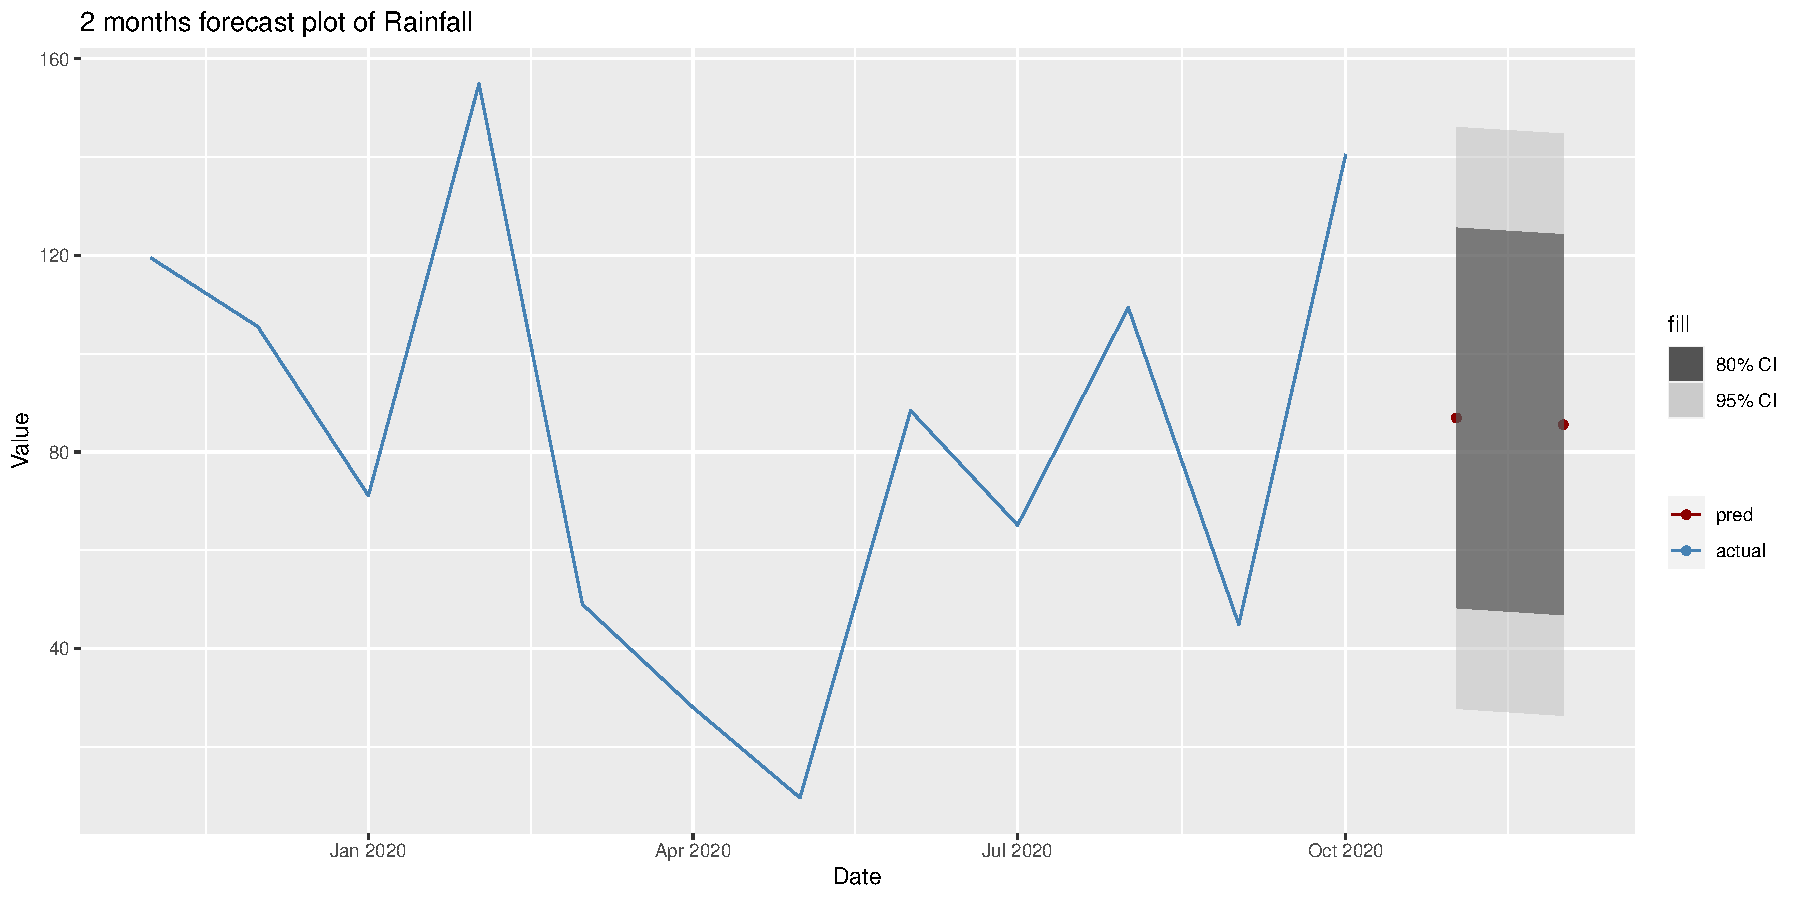
\includegraphics{ST422_files/figure-latex/unnamed-chunk-27-1.pdf}
\caption{2 Month forecasting}
\end{figure}

\begin{verbatim}
##          Point Forecast    Lo 80    Hi 80    Lo 95    Hi 95
## Nov 2020       86.92119 48.24621 125.5962 27.77291 146.0695
## Dec 2020       85.53629 46.83539 124.2372 26.34837 144.7242
\end{verbatim}

\begin{figure}
\centering
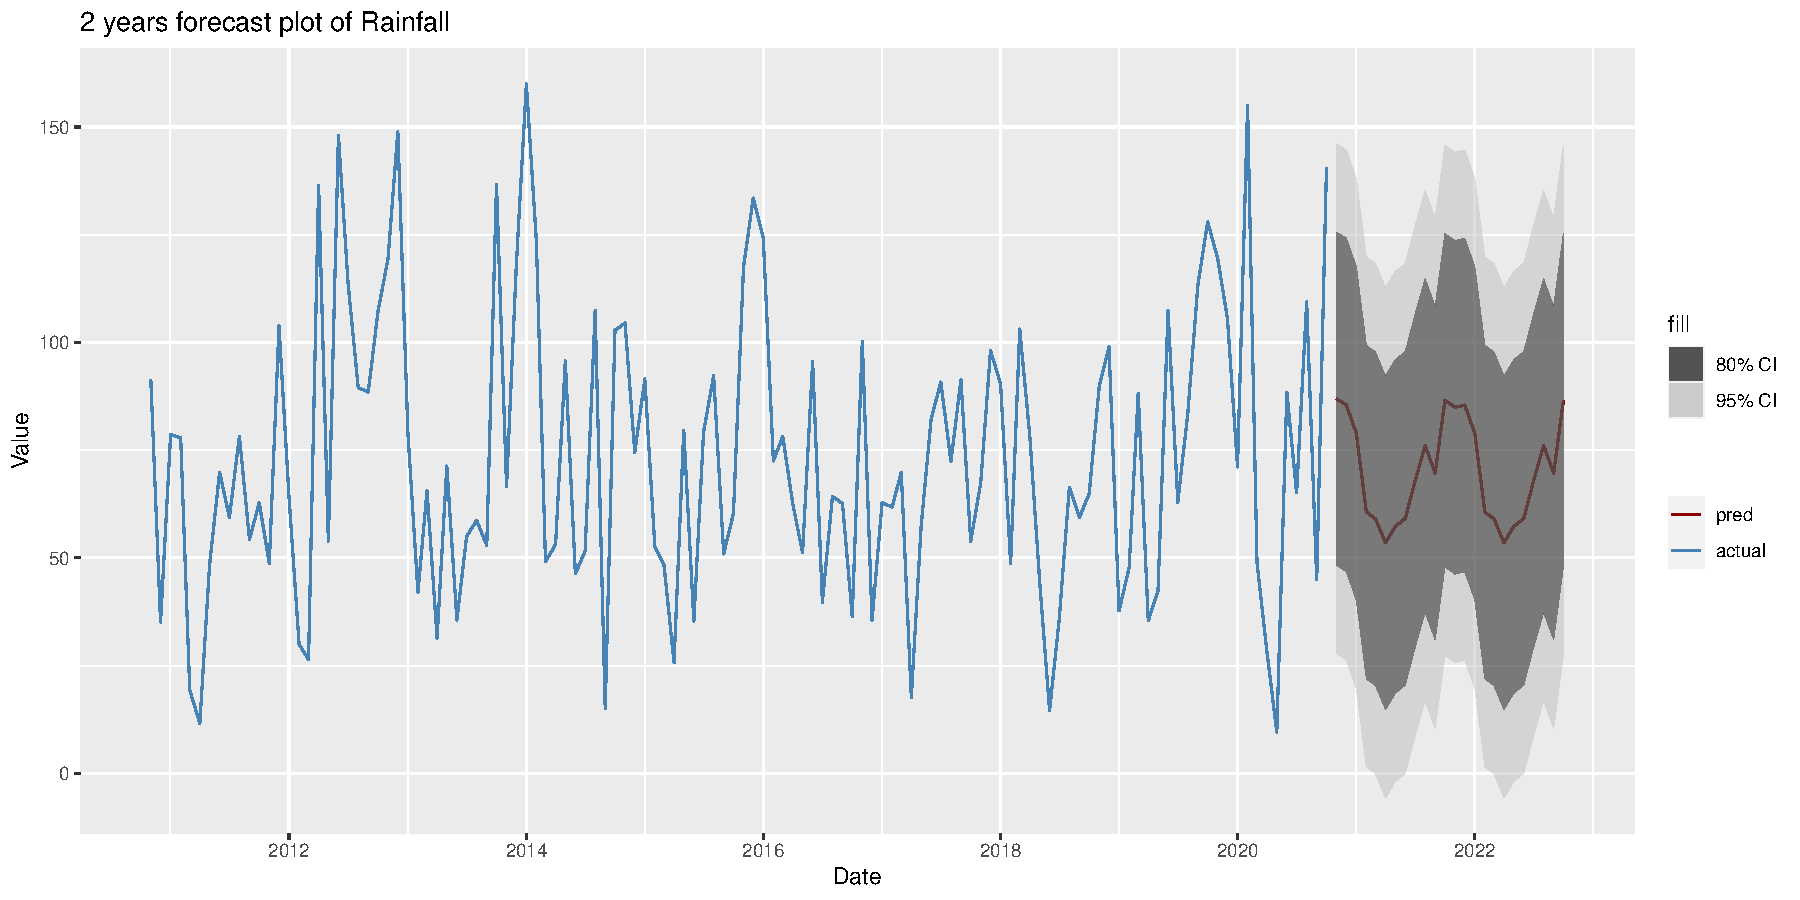
\includegraphics{ST422_files/figure-latex/unnamed-chunk-28-1.pdf}
\caption{24 Month forecasting}
\end{figure}

Based on forecast visual plots, it can be concluded that the final model
is following a general trend without any observed outlines.

\newpage
\newpage

\hypertarget{mean-temperat-series}{%
\subsection{Mean Temperat series}\label{mean-temperat-series}}

\hypertarget{preliminary-analysis-2}{%
\subsubsection{Preliminary analysis}\label{preliminary-analysis-2}}

\begin{figure}
\centering
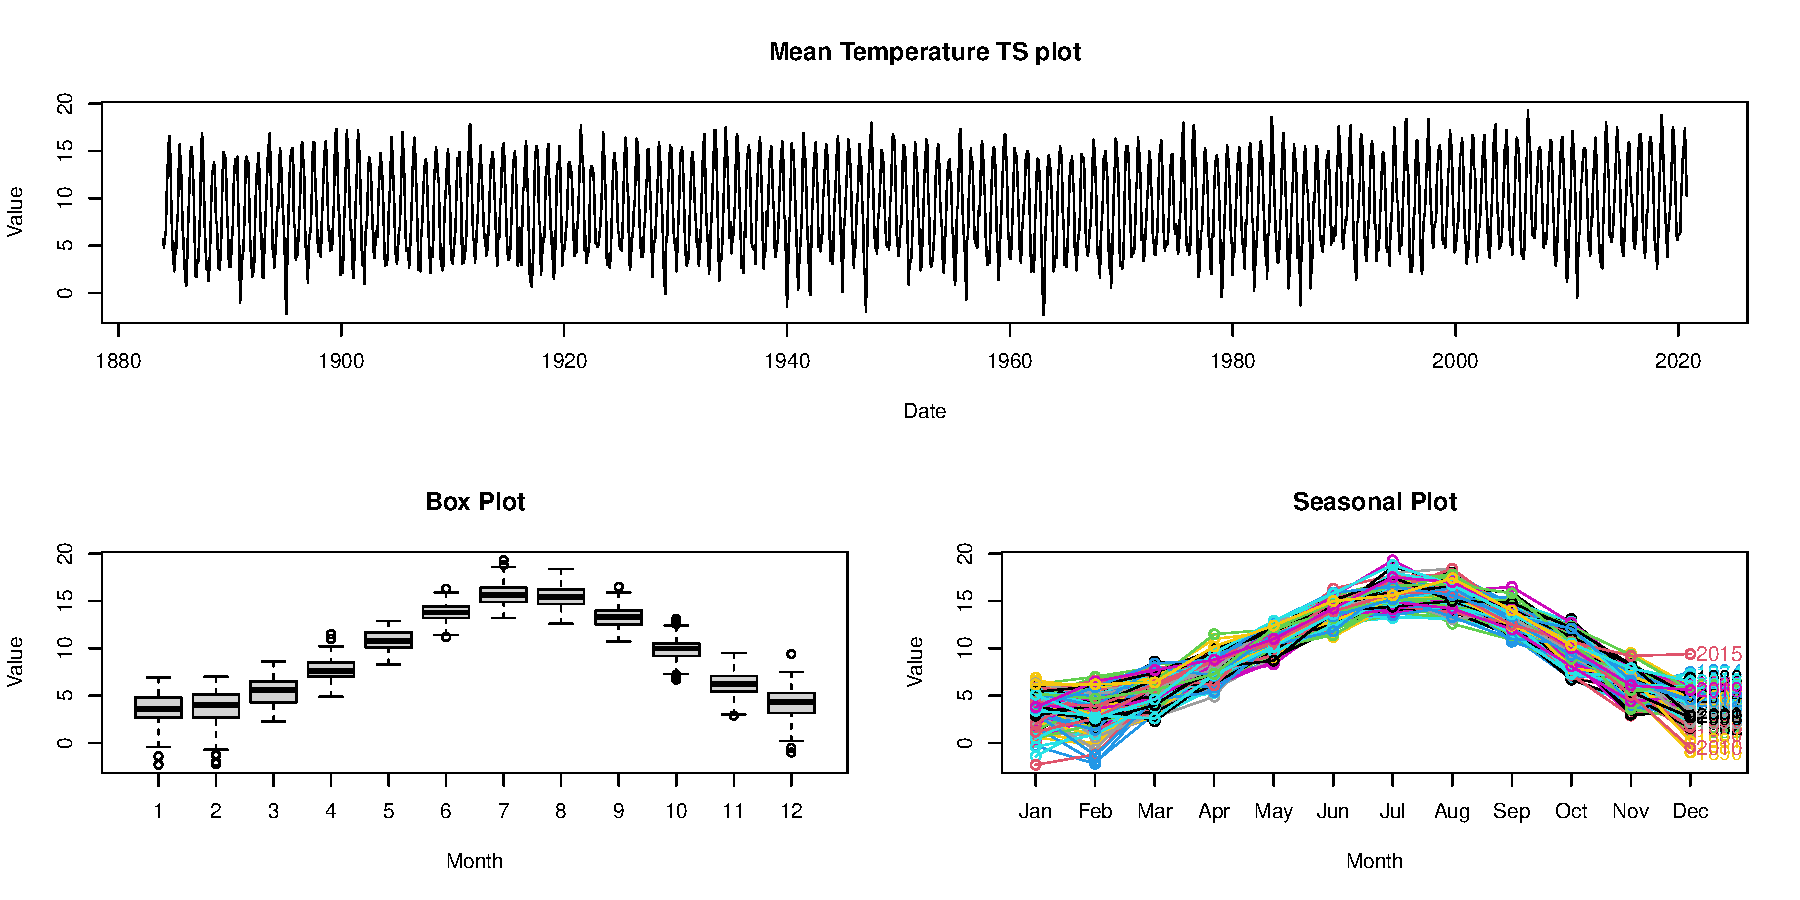
\includegraphics{ST422_files/figure-latex/unnamed-chunk-29-1.pdf}
\caption{Preliminary analysis on entire Rainfall series}
\end{figure}

\begin{figure}
\centering
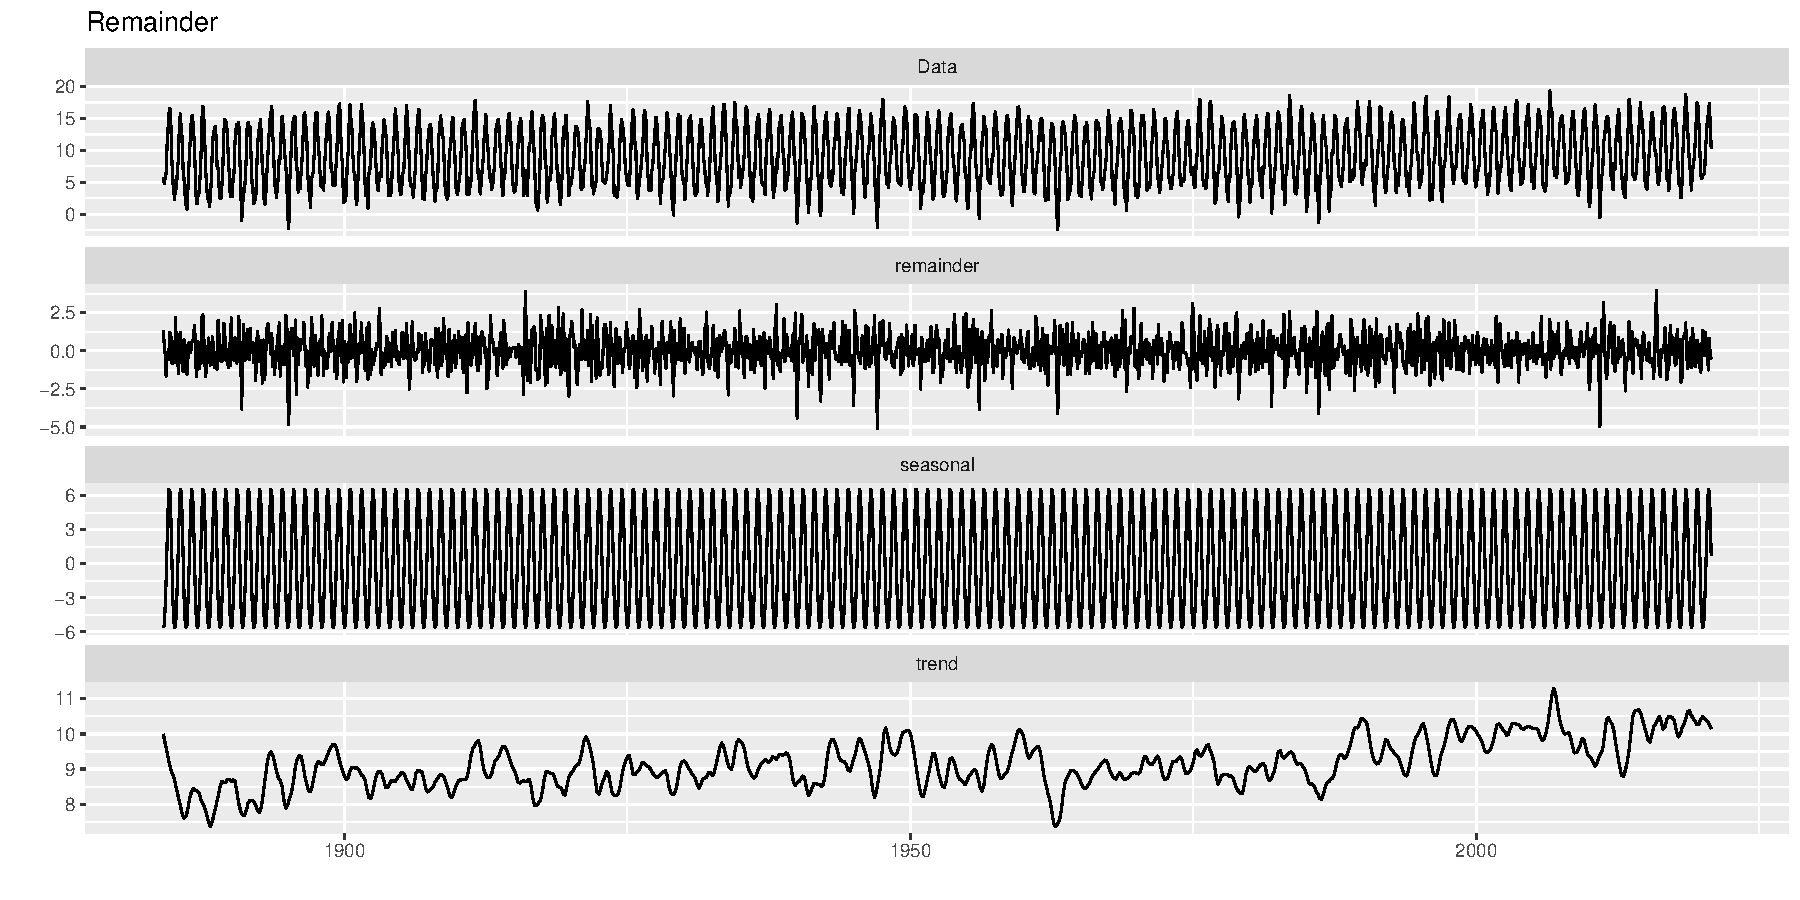
\includegraphics{ST422_files/figure-latex/unnamed-chunk-30-1.pdf}
\caption{Decomposition analysis on entire Rainfall series}
\end{figure}

By comparing the preliminary analysis based on the entire dataset
(Figure 21) and partial dataset (Figure 23), using the entire dataset is
a bit of stretch and there is no major difference in terms of the unique
patterns and trends observed between these two datasets. Hence, for
better intuitive understanding on analysis, the preliminary analysis is
conducted on the partial dataset (21st century) but the final modelling
will be using the entire population.

\newpage

\begin{figure}
\centering
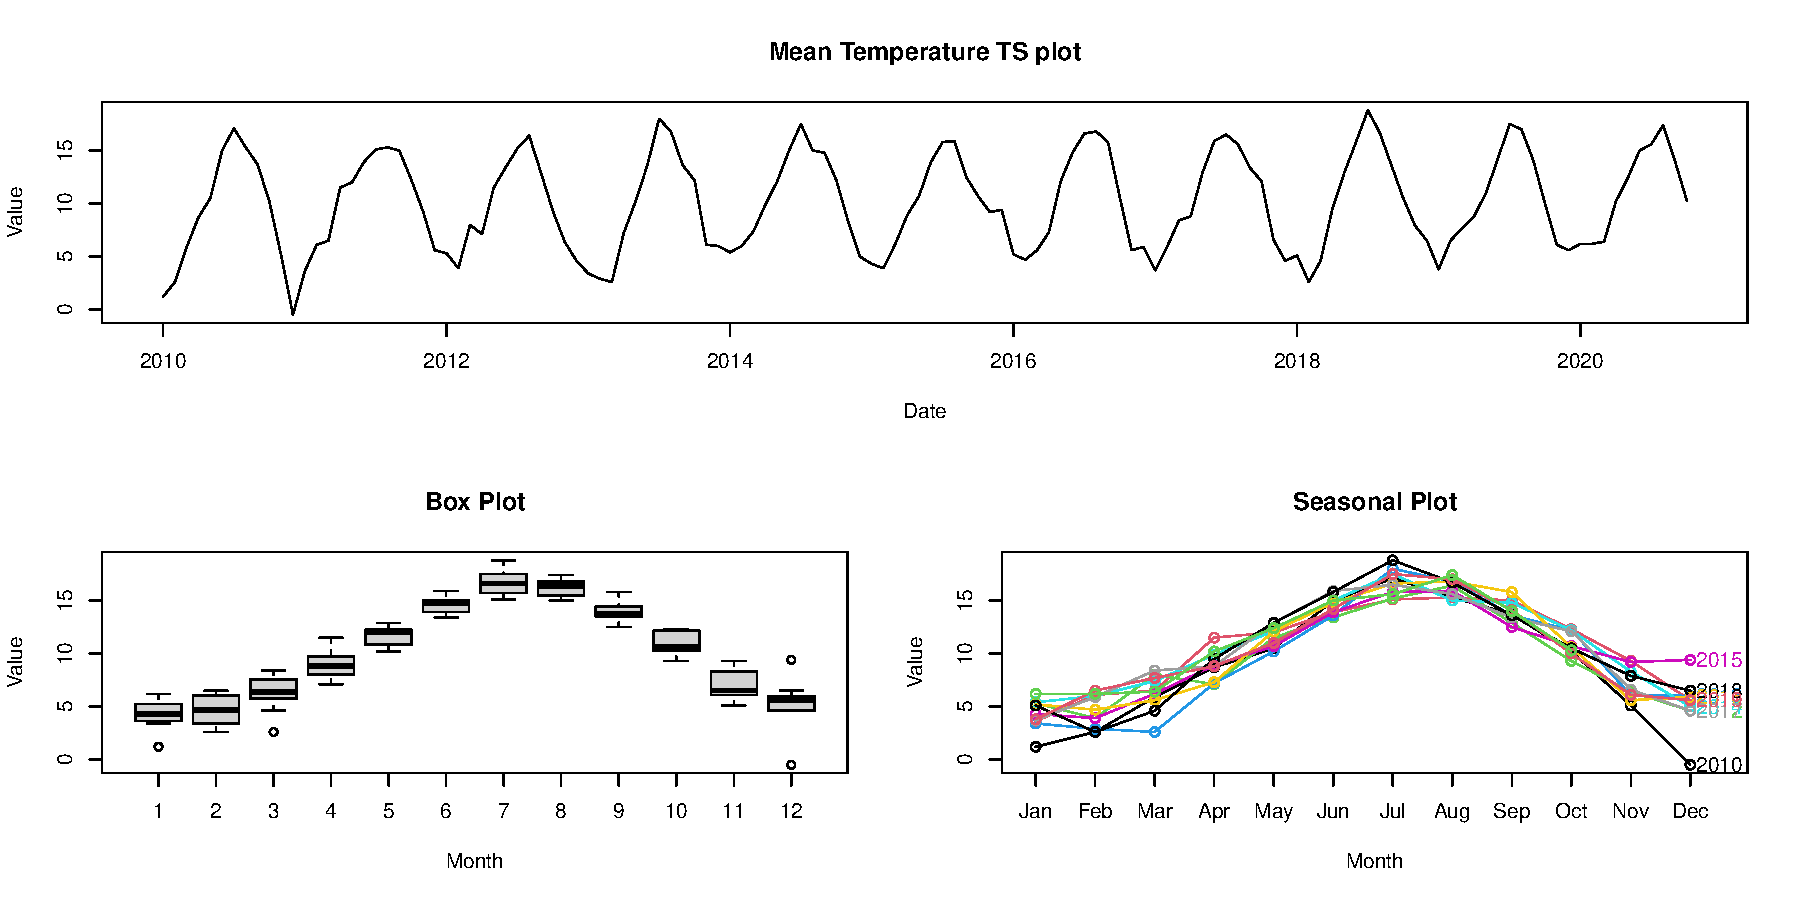
\includegraphics{ST422_files/figure-latex/unnamed-chunk-31-1.pdf}
\caption{Preliminary analysis on trimmed Mean Temperature series}
\end{figure}

\begin{figure}
\centering
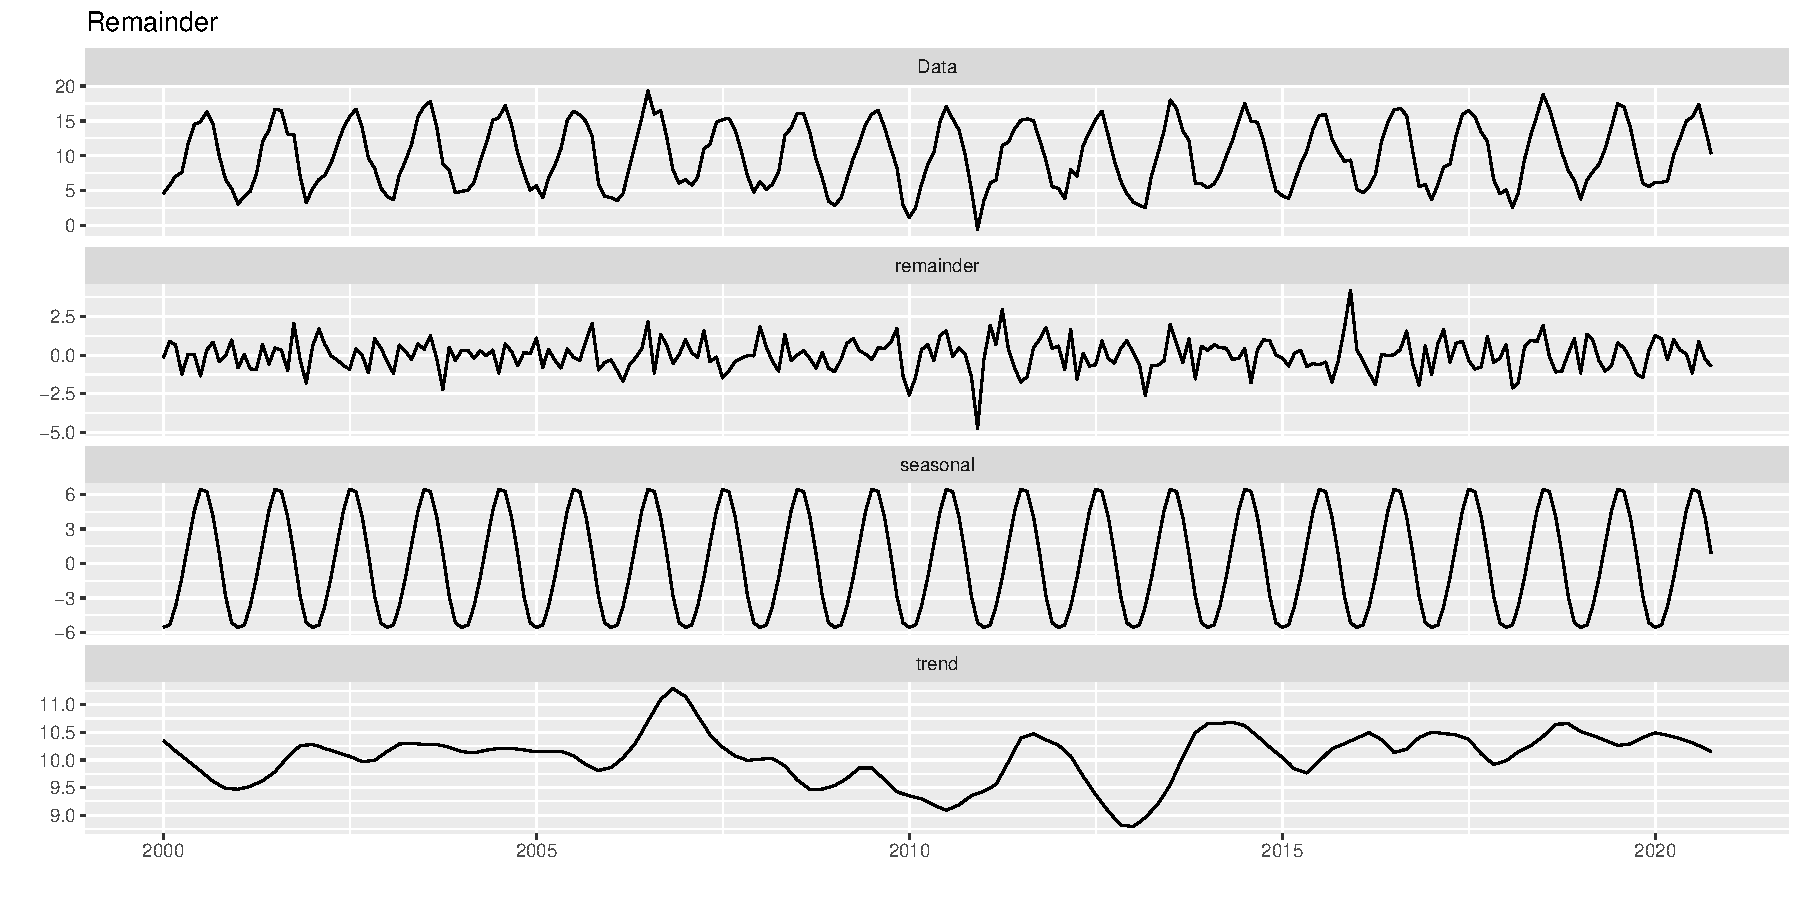
\includegraphics{ST422_files/figure-latex/unnamed-chunk-32-1.pdf}
\caption{Decomposition analysis on trimmed Mean Temperature series}
\end{figure}

Based on preliminary analysis plots on \textbf{Mean Temperature} series,
following observations are made:

\begin{enumerate}
\def\labelenumi{\arabic{enumi}.}
\tightlist
\item
  Monthly time-series plot shows high fluctuation but no visible trend
  nor increasing variance.
\item
  Box plots and seasonal plot indicate the existence of seasonal trend.
\item
  Decomposition analysis provide some additional insights that the trend
  cycle and the seasonal plot shows there's seasonal fluctuation
  occurred with no specific trend and fairly random remainder/residual.
\end{enumerate}

Conducted analysis indicate that mean temperature seems to be reach the
peak during summer (Jul \textasciitilde{} Aug) and reaches to the lowest
point during winter (Dec \textasciitilde{} Jan).

Given this observed seasonality in time series, I further delve into the
existence of seasonal persistence and the time series model
identification with ACF \& PACF plots.

\newpage

\hypertarget{acf-pacf-and-stationarity-analysis-2}{%
\subsubsection{ACF, PACF and stationarity
analysis}\label{acf-pacf-and-stationarity-analysis-2}}

\begin{figure}
\centering
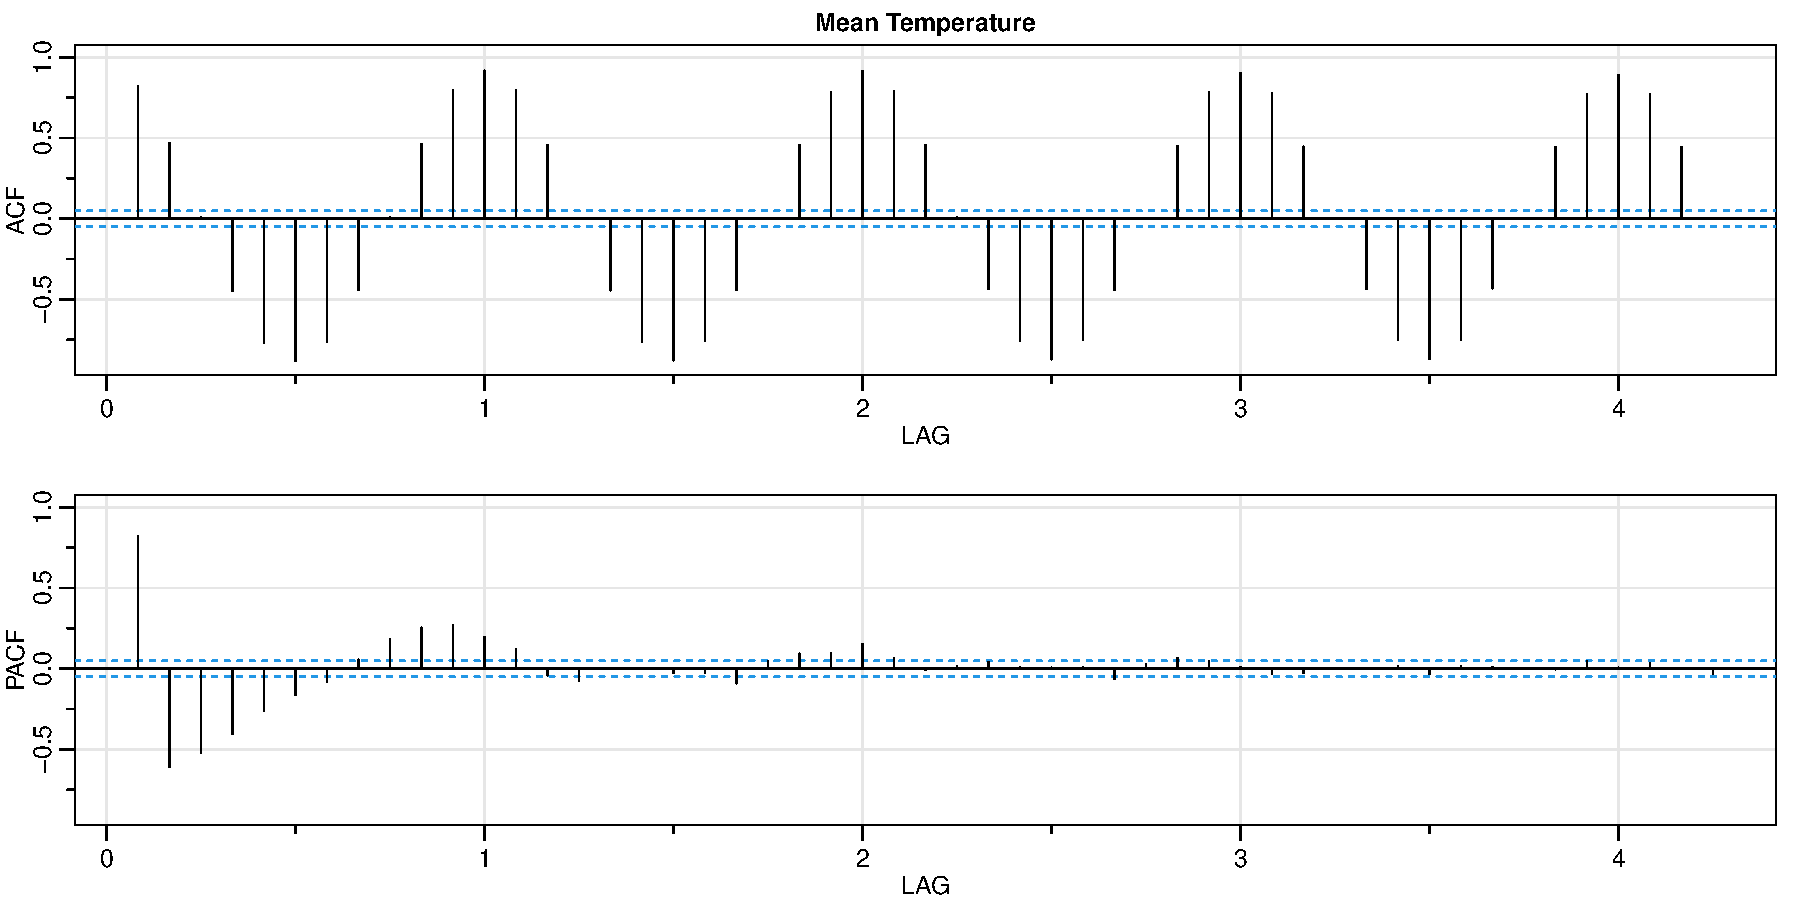
\includegraphics{ST422_files/figure-latex/unnamed-chunk-33-1.pdf}
\caption{ACF \& PACF plots of Mean Temperature series}
\end{figure}

\begin{verbatim}
## 
##  Augmented Dickey-Fuller Test
## 
## data:  ts_v
## Dickey-Fuller = -7.0541, Lag order = 12, p-value = 0.01
## alternative hypothesis: stationary
\end{verbatim}

Prior to ACF and PACF assessment, there is one of the most important
conditions required for time-series analysis that I need to check,
stationarity. Augmented Dickey-Fuller test is the most commonly used
test method to attest the stationarity of series. Based on the conducted
time-series analysis, the result could reject the null hypothesis at 5\%
significance level that the series is stationary.

In addition, based on ACF and PACF plots (Figure 25), it can verify the
existence of seasonal persistence around 12 every month and can gain
further insights and draw the blueprint of our model specification:

\begin{enumerate}
\def\labelenumi{\arabic{enumi}.}
\tightlist
\item
  ACF cuts off at lag 2 and PACF tails off -\textgreater{} MA(2)
\item
  Other model suggestion \& exploration with modifying AR and MA
  component by \(\pm1\)
\end{enumerate}

Based on seasonal pattern observed in the preliminary analysis,
consideration of a multiplicative seasonal ARIMA model is reasonable.
Our variable of interest, monthly mean temperature \(x_t\) as being
modeled as:

\[x_t = S_t + w_t\]

where \(S_t\) is a seasonal component that varies a little from one year
to the next.

As a next step, 12 month differencing is going to be examined to find a
roughly stationary series and then find a multiplicative seasonal ARIMA
to fit the resulting residual series.

\newpage

\hypertarget{nabla_12-series-analysis-2}{%
\subsubsection{\texorpdfstring{\(\nabla_{12}\) series
analysis}{\textbackslash nabla\_\{12\} series analysis}}\label{nabla_12-series-analysis-2}}

\begin{figure}
\centering
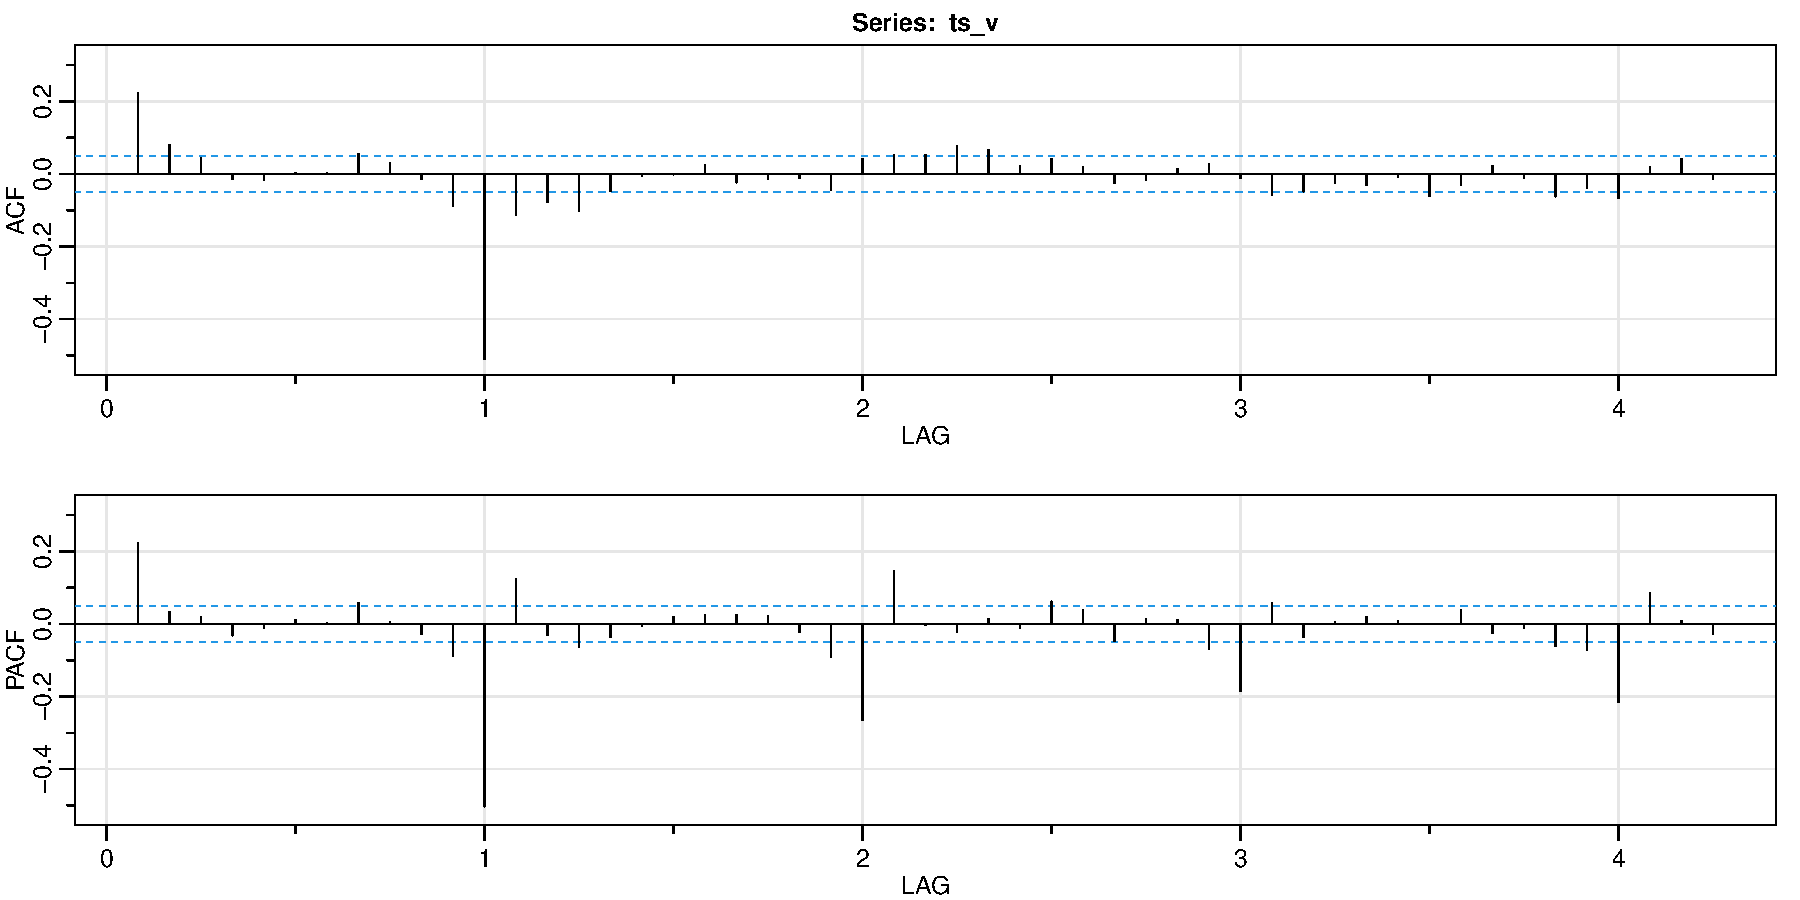
\includegraphics{ST422_files/figure-latex/unnamed-chunk-34-1.pdf}
\caption{ACF \& PACF plots of seasonally differenced Mean Temperature
series}
\end{figure}

\begin{verbatim}
## 
##  Augmented Dickey-Fuller Test
## 
## data:  ts_v
## Dickey-Fuller = -16.419, Lag order = 12, p-value = 0.01
## alternative hypothesis: stationary
\end{verbatim}

The resulting ACF and PACF (Figure 26) possibly indicate that:

\begin{enumerate}
\def\labelenumi{\arabic{enumi}.}
\tightlist
\item
  ACF cuts off at lag 1 and PACF decays quickly -\textgreater{} MA(1)
\item
  Other model suggestion \& exploration with modifying AR and MA
  component by \(\pm1\)
\end{enumerate}

\newpage

\hypertarget{model-fitting-using-sarima-2}{%
\subsubsection{Model fitting using
SARIMA}\label{model-fitting-using-sarima-2}}

In this section, I fit the optimal parameters of the time-series model
based on insights gained from previous analysis and extend the scope
with other models based on the suggestion with modifying AR and MA
component by \(\pm1\). For model exploration, an exhaustive approach
(i.e.~grid-search) will be used to calculate the goodness of fit of a
possible set models and rank them based on the performance (i.e.~AIC).
Furthermore, an additional candidate model using auto.arima() function
from the third party R package is going to be examined as well. Hence,
total 3 different specifications will be compared:

\begin{enumerate}
\def\labelenumi{\arabic{enumi}.}
\tightlist
\item
  \(ARMA(0,0,2)\times(0,1,1)_{12}\) \textless- Best guess model based on
  preliminary analysis.
\item
  Grid-search model
\item
  auto.arima() model
\end{enumerate}

Initial non-seasonal \& seasonal parameters for grid-search approach are
derived from Model 1: \(ARMA(0,0,2)\times(0,1,1)_{12}\).

\newpage

\hypertarget{model-diagnosis-and-final-model-selection-2}{%
\subsubsection{Model diagnosis and final model
selection}\label{model-diagnosis-and-final-model-selection-2}}

\begin{Shaded}
\begin{Highlighting}[]
\CommentTok{# Comparison}
\NormalTok{best_guess_mt }\CommentTok{# Best guess}
\end{Highlighting}
\end{Shaded}

\begin{verbatim}
## Series: mt_ts 
## ARIMA(0,0,2)(0,1,1)[12] 
## 
## Coefficients:
##          ma1     ma2     sma1
##       0.2550  0.0881  -0.9427
## s.e.  0.0248  0.0244   0.0095
## 
## sigma^2 estimated as 1.619:  log likelihood=-2717.19
## AIC=5442.38   AICc=5442.41   BIC=5463.97
\end{verbatim}

\begin{Shaded}
\begin{Highlighting}[]
\NormalTok{optimal_mt }\CommentTok{# Grid-search}
\end{Highlighting}
\end{Shaded}

\begin{verbatim}
## Series: mt_ts 
## ARIMA(1,0,3)(0,1,1)[12] 
## 
## Coefficients:
##          ar1      ma1      ma2      ma3     sma1
##       0.9999  -0.7540  -0.1584  -0.0692  -0.9953
## s.e.  0.0002   0.0247   0.0321   0.0248   0.0076
## 
## sigma^2 estimated as 1.554:  log likelihood=-2694.7
## AIC=5401.4   AICc=5401.45   BIC=5433.78
\end{verbatim}

\begin{Shaded}
\begin{Highlighting}[]
\NormalTok{auto_arima_mt }\CommentTok{# auto.arima}
\end{Highlighting}
\end{Shaded}

\begin{verbatim}
## Series: mt_ts 
## ARIMA(1,0,0)(2,1,0)[12] 
## 
## Coefficients:
##          ar1     sar1     sar2
##       0.2535  -0.6820  -0.3117
## s.e.  0.0240   0.0236   0.0237
## 
## sigma^2 estimated as 2.062:  log likelihood=-2904.27
## AIC=5816.53   AICc=5816.56   BIC=5838.12
\end{verbatim}

Resulted 3 different models can be found below:

\begin{enumerate}
\def\labelenumi{\arabic{enumi}.}
\tightlist
\item
  \(ARMA(0,0,2)\times(0,1,1)_{12}\) \textless- Model(1) Best guess
\item
  \(ARMA(1,0,3)\times(0,1,1)_{12}\) \textless- Model(2) Grid-search
\item
  \(ARMA(1,0,0)\times(2,1,0)_{12}\) \textless- Model(3) auto.arima
\end{enumerate}

Based on the goodness of fit metrics of 3 different models, Model(2)
provides the best model fit with all significant coefficients :
\(ARMA(1,0,3)\times(0,1,1)_{12}\).

\begin{figure}
\centering
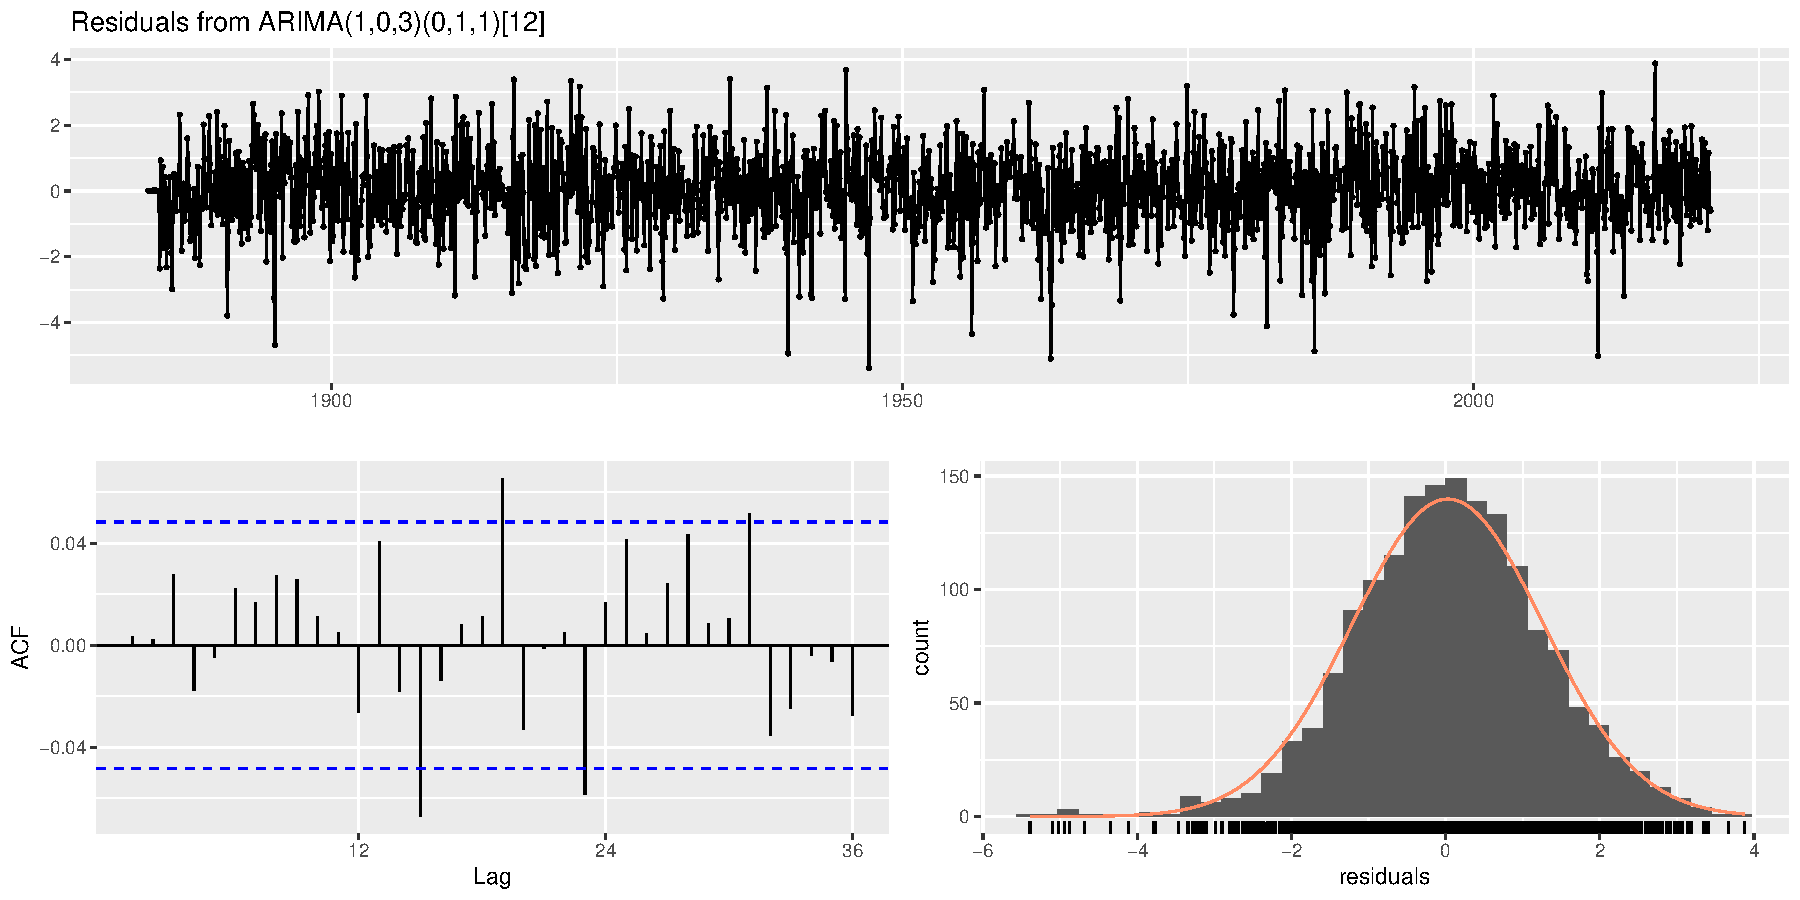
\includegraphics{ST422_files/figure-latex/unnamed-chunk-37-1.pdf}
\caption{Residual diagnosis}
\end{figure}

\begin{verbatim}
## 
##  Ljung-Box test
## 
## data:  Residuals from ARIMA(1,0,3)(0,1,1)[12]
## Q* = 33.491, df = 19, p-value = 0.02108
## 
## Model df: 5.   Total lags used: 24
\end{verbatim}

\begin{figure}
\centering
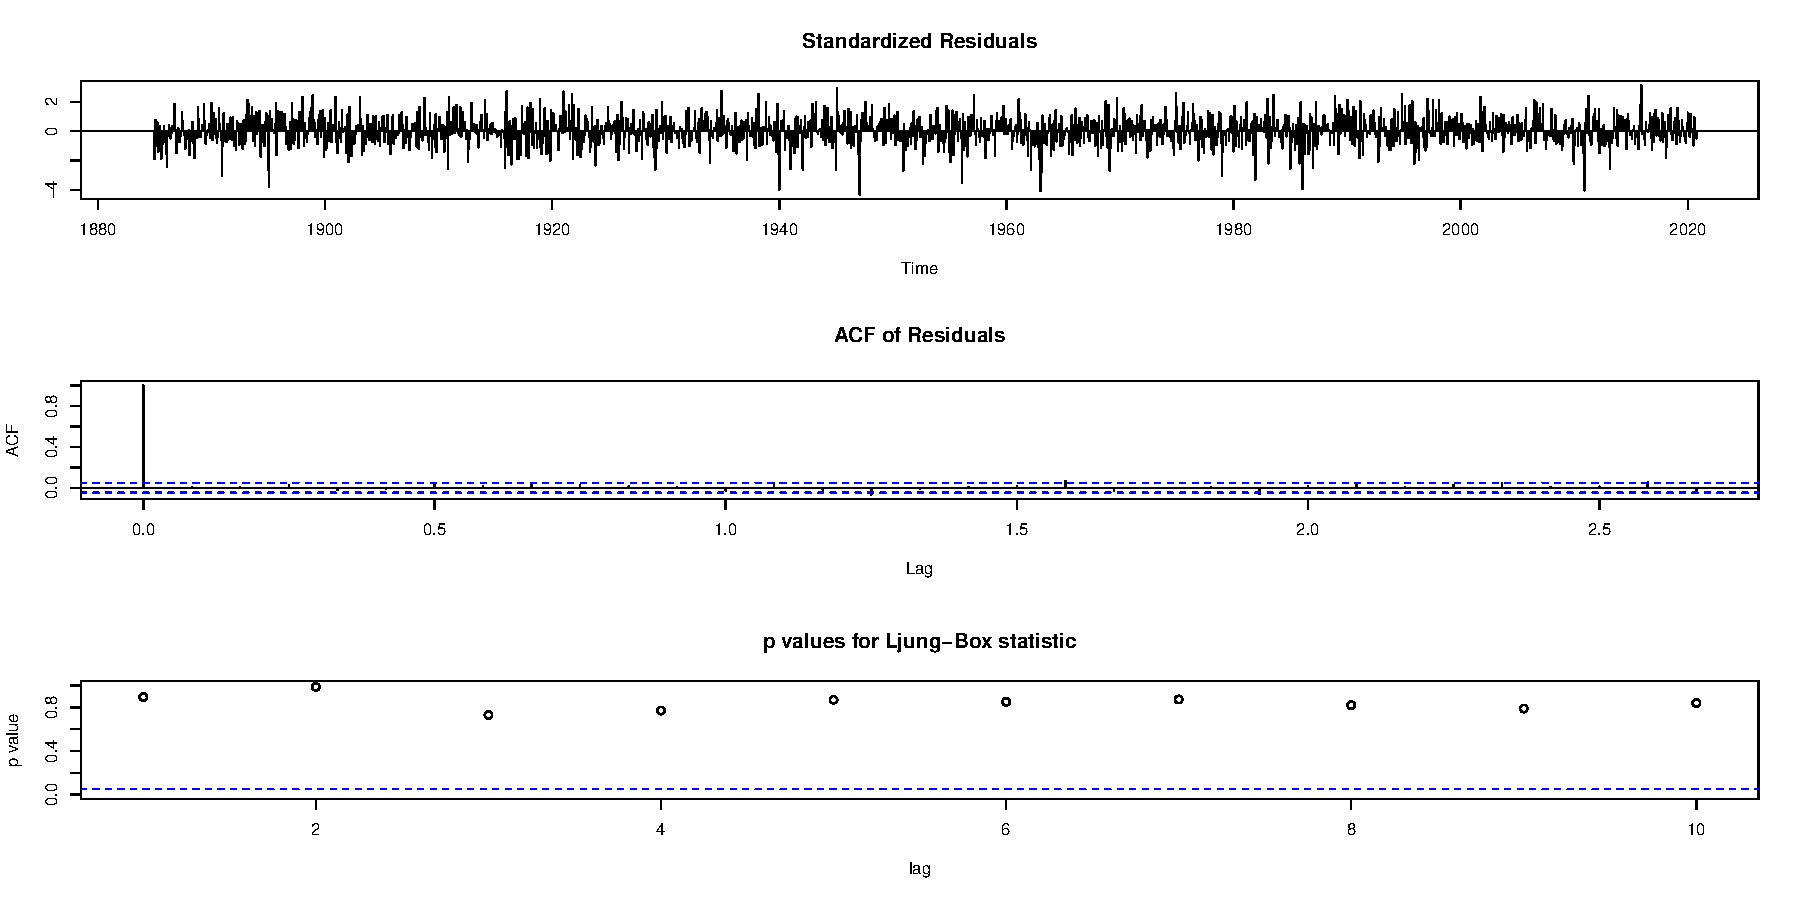
\includegraphics{ST422_files/figure-latex/unnamed-chunk-37-2.pdf}
\caption{Residual diagnosis}
\end{figure}

Based on the Ljung-Box test and ACF plot of model residuals (Figure 27
\& 28), it can be concluded that this model is appropriate for
forecasting since its residuals show white noise behavior and
uncorrelated against each other.

\newpage

\hypertarget{model-forecasting-2}{%
\subsubsection{Model forecasting}\label{model-forecasting-2}}

As a finale, I plot 2 months forecasting plot and 24 months forecast
plot to inspect the behaviour of estimated values.

\begin{figure}
\centering
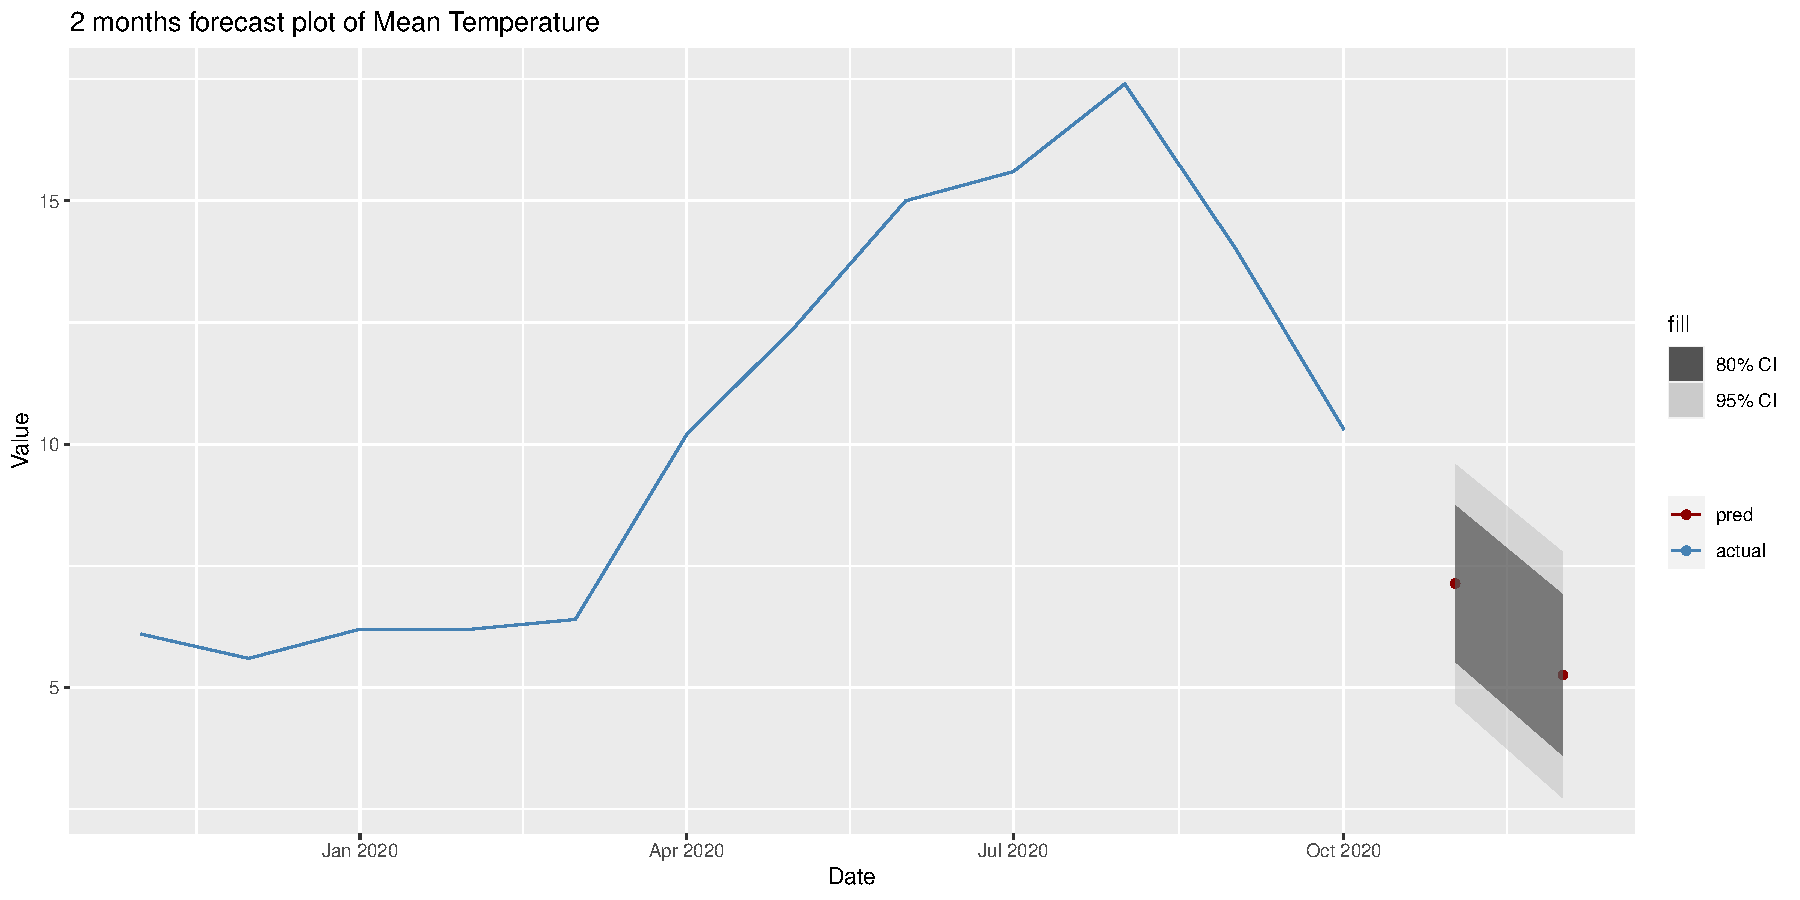
\includegraphics{ST422_files/figure-latex/unnamed-chunk-38-1.pdf}
\caption{2 Month forecasting}
\end{figure}

\begin{verbatim}
##          Point Forecast    Lo 80    Hi 80    Lo 95    Hi 95
## Nov 2020       7.138369 5.537849 8.738889 4.690585 9.586153
## Dec 2020       5.257024 3.608838 6.905209 2.736341 7.777706
\end{verbatim}

Based on forecast visual plots below, it can be concluded that the final
model is following a general trend without any observed outlines.

\begin{figure}
\centering
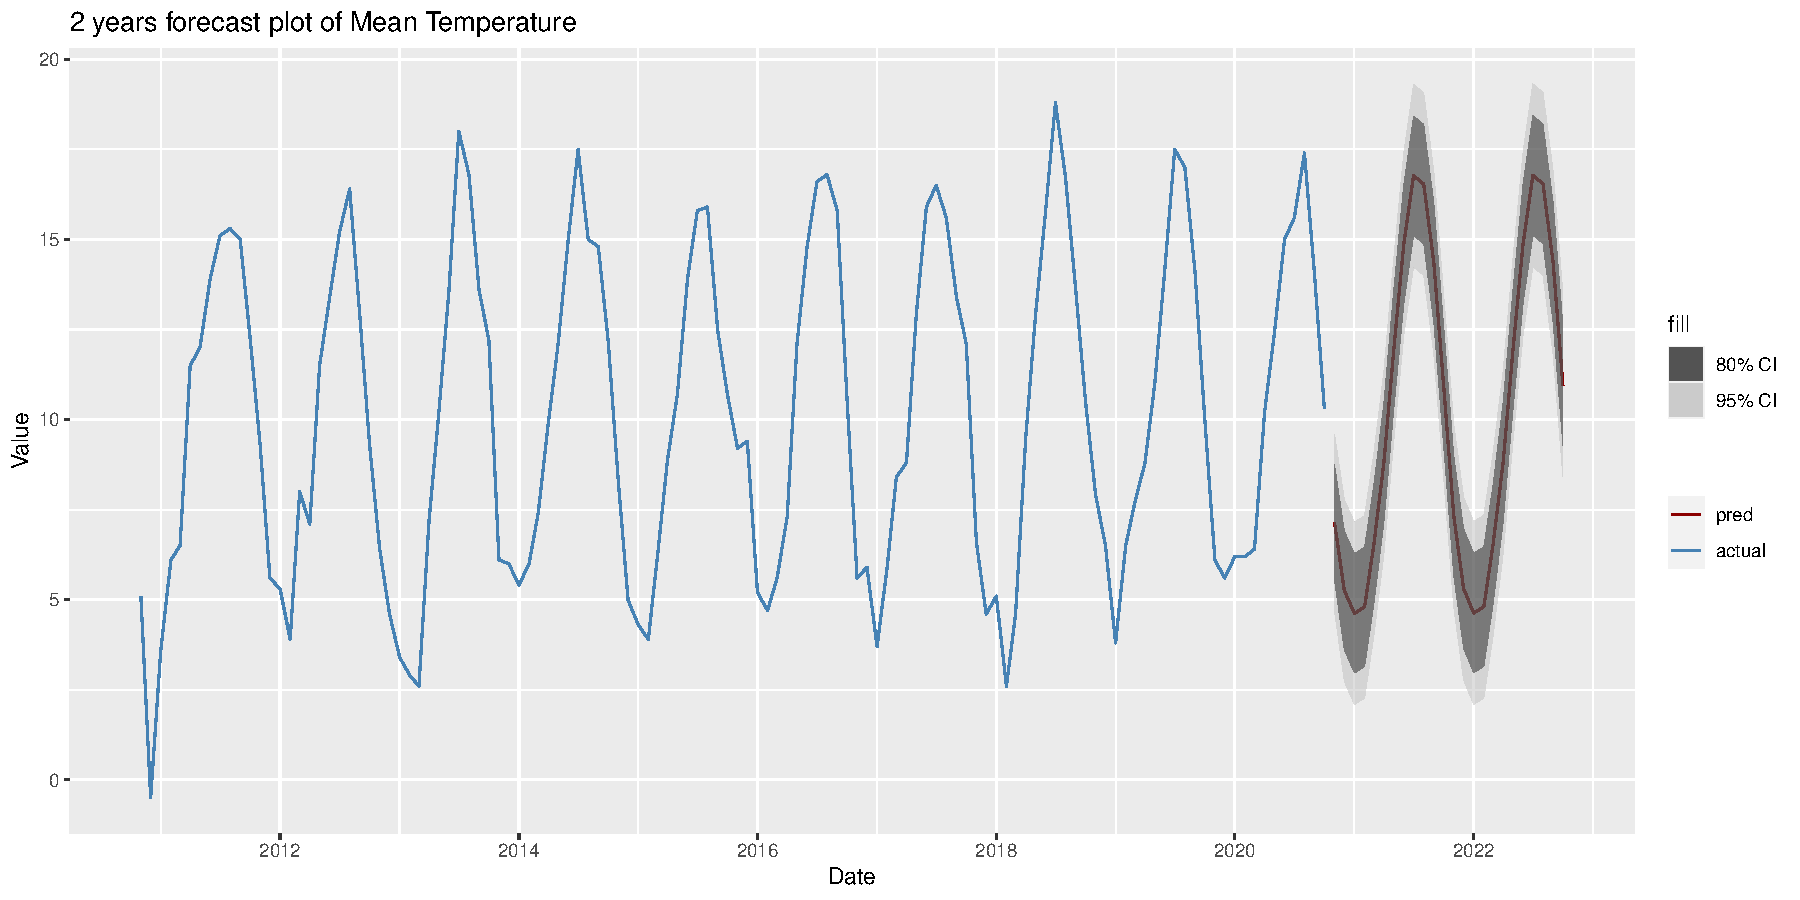
\includegraphics{ST422_files/figure-latex/unnamed-chunk-39-1.pdf}
\caption{24 Month forecasting}
\end{figure}

\newpage

\hypertarget{q3-rolling-window}{%
\section{Q3: Rolling Window}\label{q3-rolling-window}}

\hypertarget{description}{%
\subsection{Description}\label{description}}

Various rolling window approaches are considered in this section. Given
the sheer amount of dataset available for modelling, a list of rolling
windows for model development (i.e.~fitting), ``M'' is considered and a
fixed value of validation window (i.e.~forecast \& comparison against
the actual values), ``A'' is considered to find the optimal rolling
window length.

With a fixed value of ``A'', the larger ``M'' value is expected to fit
the model with lower error as larger sample sizes give more reliable
results with greater precision and power. Hence, various rolling windows
for model development (M = 36, 72, 108, 144, 180; 3 years increment up
to 15 years) are considered for the robust result.

Having a larger validation window (A) reduces the number of required
iteration for model refitting. Furthermore, the shorter interval of
validation window is introduced, the more frequent model refitting is
needed. This could lead to one of menaces of statistical model
development, the model over-fitting. In addition, having a long
validation window is not expected to compromise the final outcome given
the size of dataset available (More than 100 years). Hence, the fixed
value of \textbf{3 years} is deployed for the model validation window
(A), parallel to the increment size of rolling window ``M''.

\hypertarget{results}{%
\subsection{Results}\label{results}}

\hypertarget{sunshine}{%
\subsubsection{Sunshine}\label{sunshine}}

\begin{longtable}[]{@{}rrrr@{}}
\caption{Optimal window searching result for Sunshine (Validation
period, A = 36)}\tabularnewline
\toprule
Window & Sample & RMSE & MAE\tabularnewline
\midrule
\endfirsthead
\toprule
Window & Sample & RMSE & MAE\tabularnewline
\midrule
\endhead
36 & 916 & 38.08084 & 28.94121\tabularnewline
36 & 306 & 35.30199 & 26.46222\tabularnewline
72 & 916 & 31.68964 & 23.74663\tabularnewline
72 & 306 & 29.48377 & 21.53583\tabularnewline
108 & 916 & 29.17757 & 21.74045\tabularnewline
108 & 306 & 28.33817 & 20.49545\tabularnewline
144 & 916 & 29.38550 & 21.70412\tabularnewline
144 & 306 & 27.73625 & 20.02084\tabularnewline
180 & 916 & 30.35056 & 22.39793\tabularnewline
180 & 306 & 30.73793 & 22.68594\tabularnewline
\bottomrule
\end{longtable}

Based on the optimal window searching result for Rainfall, Train sample
(Sample=916) has the lowest RMSE value when M=108 whereas Test sample
(Sample=306) shows the lowest at M=144 The observed difference of Train
RMSE between M=108 (29.17757) and M=144 (29.38550) is marginal. Given
M=144 shows a much smaller RMSE value (32.25016) for Test dataset, it is
concluded that \textbf{M=144} is the most optimal window value for
Sunshine series.

\hypertarget{rainfall}{%
\subsubsection{Rainfall}\label{rainfall}}

\begin{longtable}[]{@{}rrrr@{}}
\caption{Optimal window searching result for Rainfall (Validation
period, A = 36)}\tabularnewline
\toprule
Window & Sample & RMSE & MAE\tabularnewline
\midrule
\endfirsthead
\toprule
Window & Sample & RMSE & MAE\tabularnewline
\midrule
\endhead
36 & 1429 & 33.27800 & 26.71494\tabularnewline
36 & 477 & 40.19060 & 33.33170\tabularnewline
72 & 1429 & 32.06189 & 25.59037\tabularnewline
72 & 477 & 32.25016 & 26.35830\tabularnewline
108 & 1429 & 31.92845 & 25.50503\tabularnewline
108 & 477 & 32.41124 & 26.41661\tabularnewline
144 & 1429 & 32.04302 & 25.54894\tabularnewline
144 & 477 & 32.65402 & 26.59269\tabularnewline
180 & 1429 & 31.95238 & 25.41482\tabularnewline
180 & 477 & 32.47736 & 26.40725\tabularnewline
\bottomrule
\end{longtable}

Based on the optimal window searching result for Rainfall, Train sample
(Sample=1429) has the lowest RMSE value when M=108 whereas Test sample
(Sample=477) shows the lowest at M=72 The observed difference of Train
RMSE between M=108 (31.92845) and M=72 (32.06189) is marginal. Given
M=72 shows a much smaller RMSE value (32.25016) for Test dataset, it is
concluded that \textbf{M=72} is the most optimal window value for
Rainfall series.

\hypertarget{mean-temperature}{%
\subsubsection{Mean Temperature}\label{mean-temperature}}

The result of Mean Temperature follows:

\begin{longtable}[]{@{}rrrr@{}}
\caption{Optimal window searching result for Mean Temperature
(Validation period, A = 36)}\tabularnewline
\toprule
Window & Sample & RMSE & MAE\tabularnewline
\midrule
\endfirsthead
\toprule
Window & Sample & RMSE & MAE\tabularnewline
\midrule
\endhead
36 & 1231 & 1.719416 & 1.346605\tabularnewline
36 & 411 & 1.830766 & 1.480863\tabularnewline
72 & 1231 & 1.490044 & 1.165079\tabularnewline
72 & 411 & 1.362905 & 1.090364\tabularnewline
108 & 1231 & 1.477336 & 1.153452\tabularnewline
108 & 411 & 1.357849 & 1.095313\tabularnewline
144 & 1231 & 1.446246 & 1.125278\tabularnewline
144 & 411 & 1.298890 & 1.052184\tabularnewline
180 & 1231 & 1.467112 & 1.143347\tabularnewline
180 & 411 & 1.367413 & 1.111805\tabularnewline
\bottomrule
\end{longtable}

Based on the optimal window searching result for Mean Temperature, the
appropriate window value is \textbf{144} considering the lowest values
of RMSE \& MAE values of both Train (N=1231) and Test (N=411) samples.

\hypertarget{forecasting}{%
\subsection{Forecasting}\label{forecasting}}

Established on the above rolling window iteration analysis, 2 months
forecast (2020 Nov \& Dec) values are derived with selected window
lengths of ``M'' for each time series. Being consistent with the rolling
window iteration analysis method, auto.arima() function is deployed to
fit the model for the 2 months ahead forecasts production.

Predicated on the below forecast plots, it is observed that the
foretasted values of the rolling window approach are not significantly
different (Within 80\% C.I.) compared to the predicted value derived on
Question 2 using SARIMA model.

\newpage

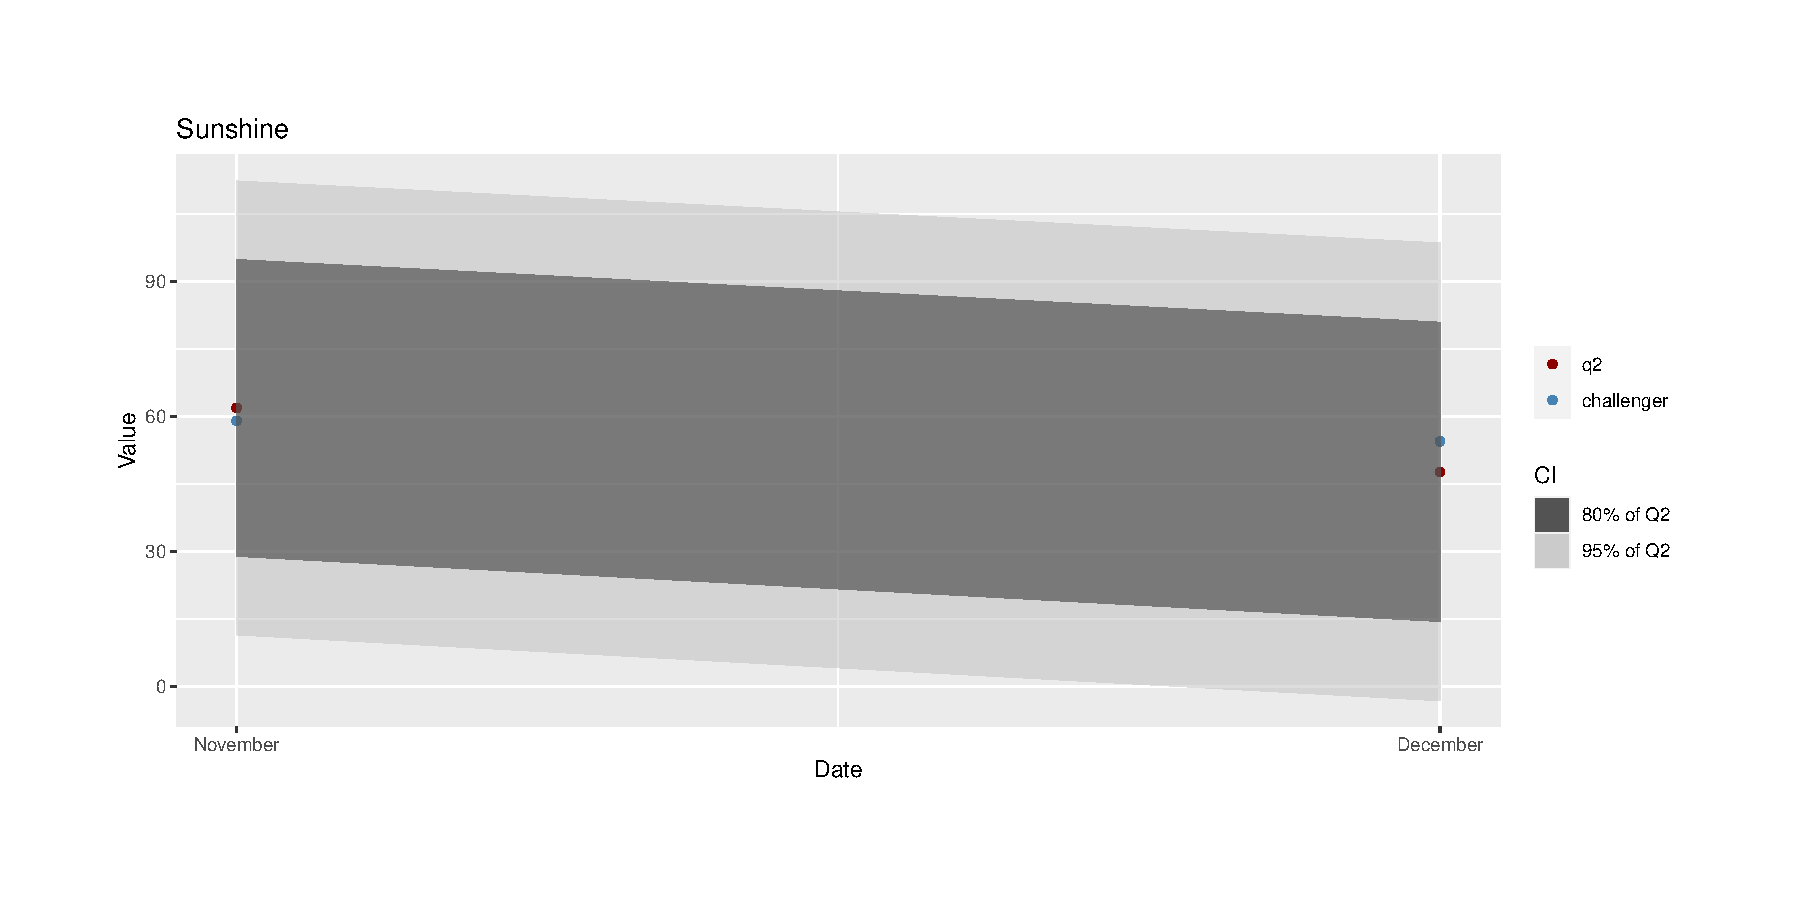
\includegraphics{ST422_files/figure-latex/unnamed-chunk-45-1.pdf}
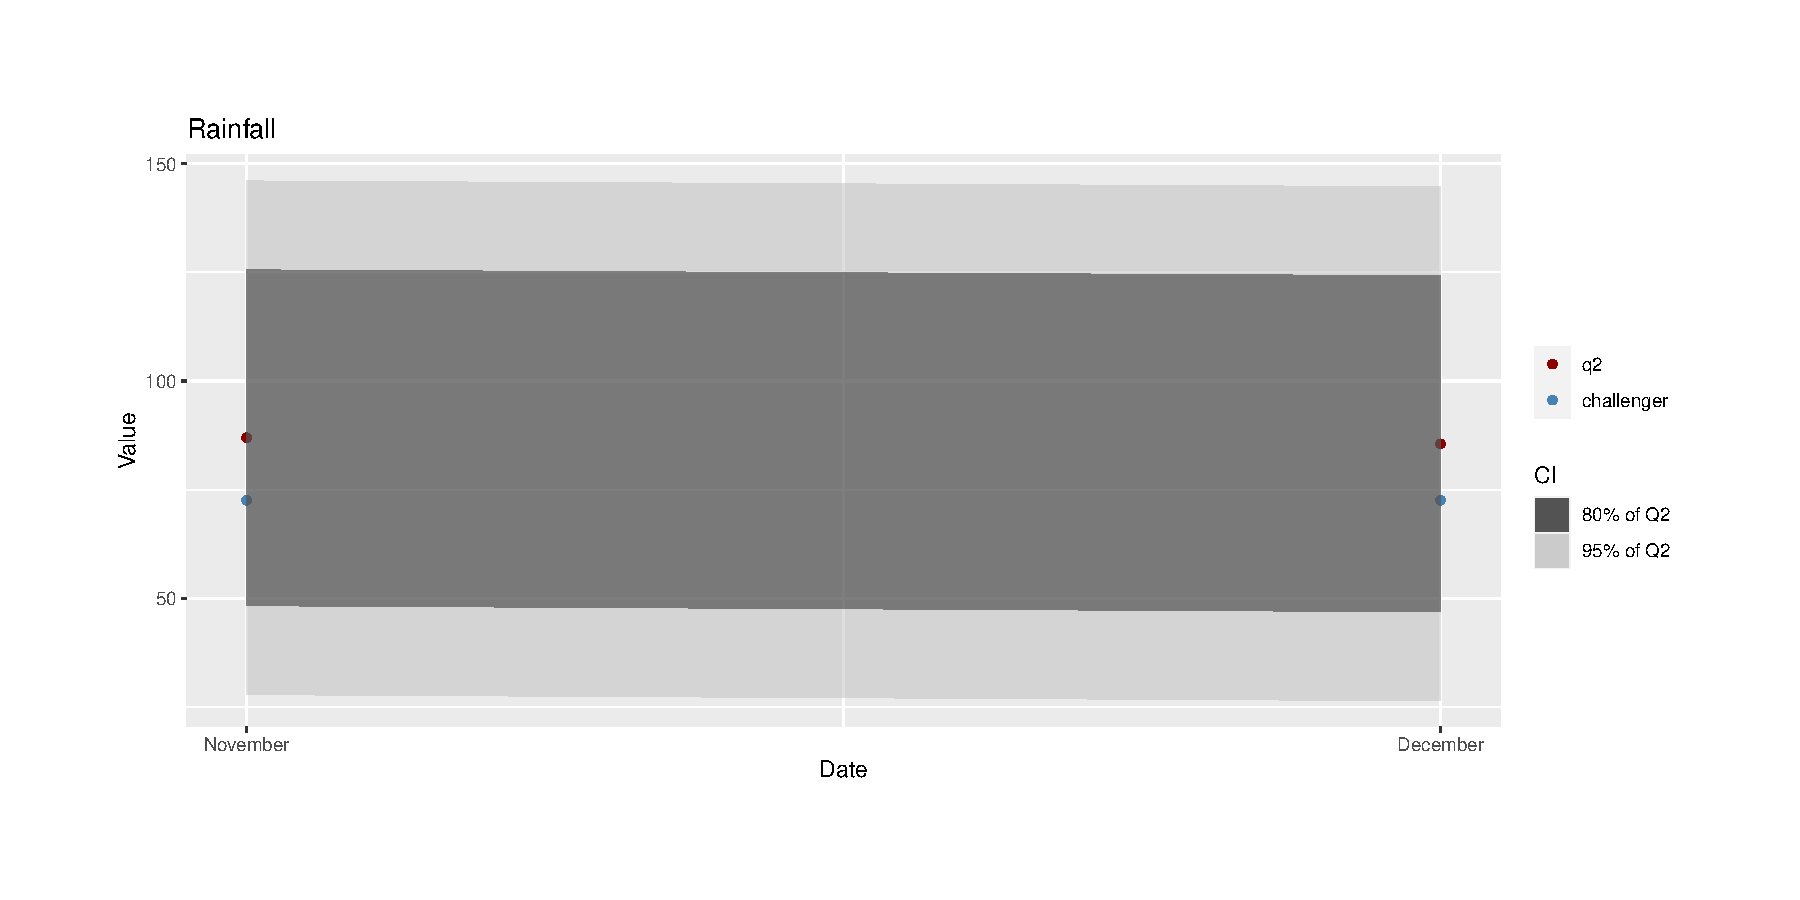
\includegraphics{ST422_files/figure-latex/unnamed-chunk-46-1.pdf}
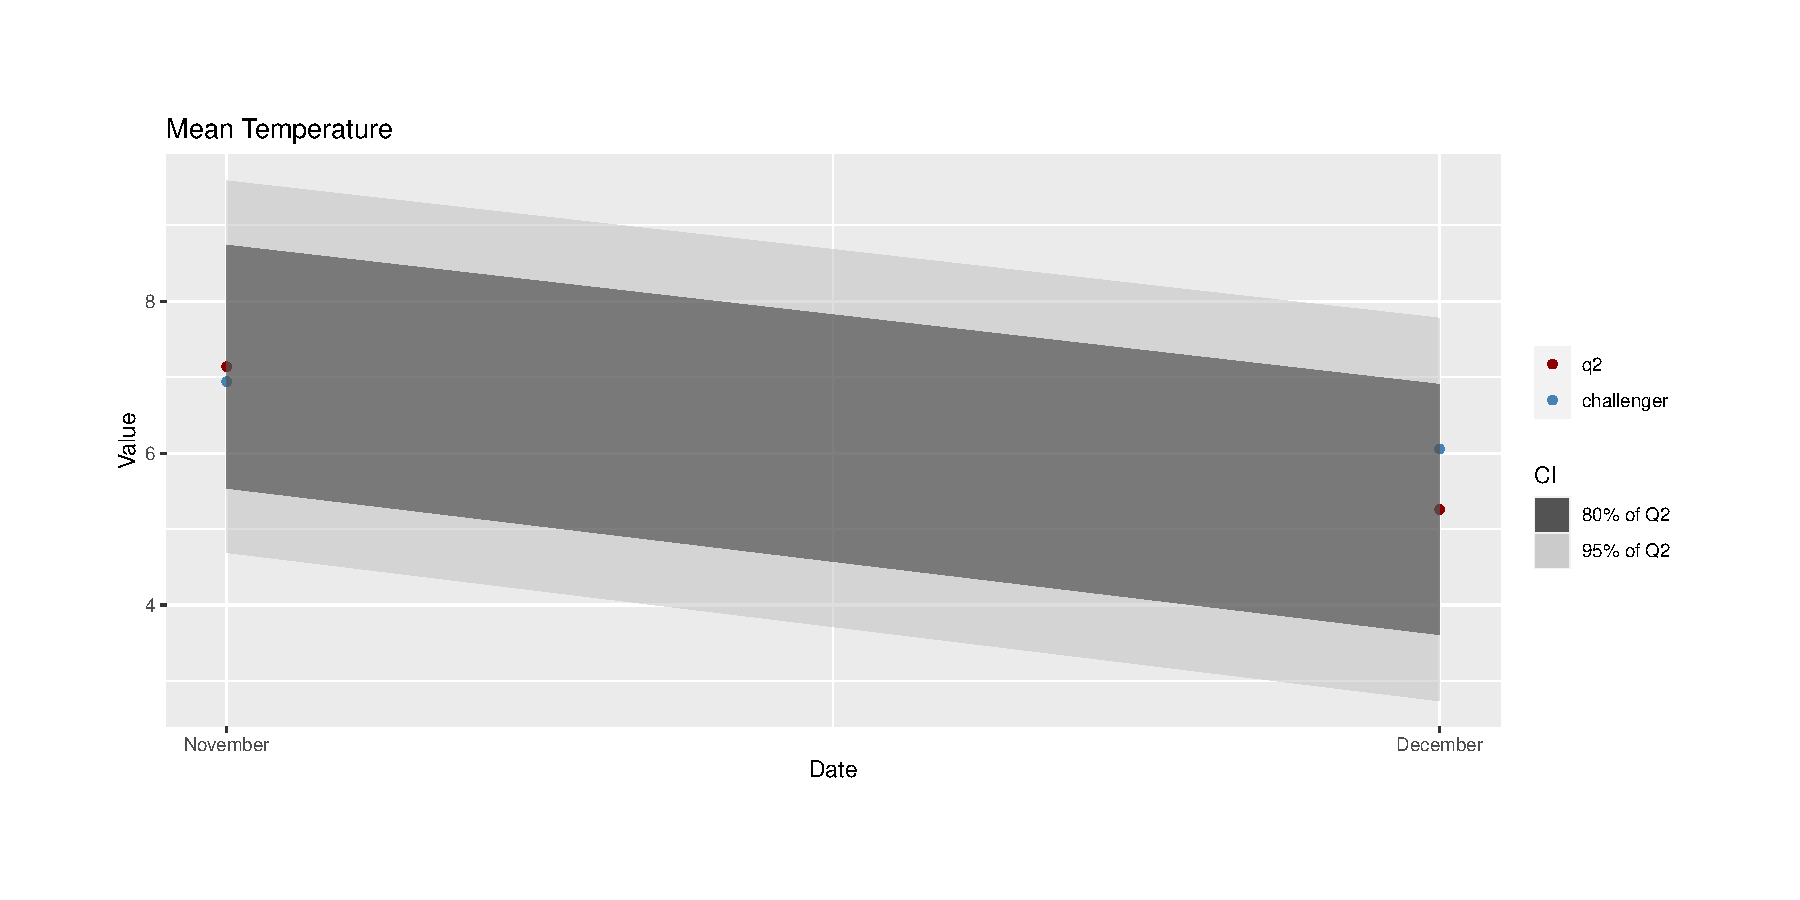
\includegraphics{ST422_files/figure-latex/unnamed-chunk-47-1.pdf}

\newpage

\hypertarget{q4-varma}{%
\section{Q4: VARMA}\label{q4-varma}}

\hypertarget{description-1}{%
\subsection{Description}\label{description-1}}

As a brief introduction, a multivariate process of ARMA is commonly
described as a VARMA process---the initial letter denoting ``vector''.
In other terms, VARMA is an extended version of finite order VAR model.
VARMA model is used to develop multivariate time series models which
allow the users to study the dynamic relationships between multiple
variables. This modelling technique allows the error terms to be
autocorrelated rather than a white noise process as in VAR.

General form of VARMA(p,q) process can be represented as: \begin{align}
  y_{t} = v+A_{1}y_{t-1}+...+A_{p}y_{,t-p}+M_{1}e_{t-1}+...+M_{q}e_{,t-q}
\end{align} where \(A_0, A_1, ..., A_p\) are AR parameter matrices,
\(M_0, M_1, ..., M_p\) are MA parameter matrices and \(e_t\) is a
white-noise process with zero mean, nonsingular, time-invariant
covariance matrix.

The function `sVARMA' included in `MTS v 1.0' package is chosen for the
model fitting function. The custom grid-search function will be
re-deployed to fit the model in a more robust manner. This custom
grid-search function will modify AR and MA component by \(\pm1\).

The required amount of CPU-energy and processing time for finding the
optimal window length and fitting the model under the rolling-window
approach is expected to outstrip what is required for the vanilla
approach. Considering sheer amount of available data for model
development, the difference in goodness of model-fit between the vanilla
and rolling-window approach is expected to be immaterial. Hence, it is
decided not to implement the rolling window approach.

As a data cleansing process, each individual variables is needed to
share the same length without any omitted values. Hence, the observed
date of the final combined design matrix is from Jan 1919 to Oct 2020.

\hypertarget{model-fitting-process}{%
\subsection{Model fitting process}\label{model-fitting-process}}

Considering the preliminary analysis conducted for each individual
variables in previous sections, it is reasonable to set a multiple model
assumptions that:

\begin{enumerate}
\def\labelenumi{\arabic{enumi}.}
\tightlist
\item
  There is a seasonality with 12 month frequency.
\item
  Seasonal component is an integrated process, hence d = 1.
\item
  There is no trend observed for non-seasonal component.
\end{enumerate}

To begin with, the results of univariate SARIMA models in Question 2
need to be re-examined. Considering all series (Sunshine, Rainfall and
Mean Temperature) are sharing the same seasonal MA(1) component, it is
reasonable to deploy MA(1) for the seasonal component for sVARMA model
and extending the grid-search hinged on this starting point.

In addition, the starting point of non-seasonal component (p,q,d) is
arbitrally set to be (1,0,1), which will give us the largest combination
of \((1\pm1, 0, 1\pm1)\) for an extensive model combination of
grid-search.

Rolling window approach in Question 3 is not considered due to the
observed fact that the optimal window lengths of each series are not
identical to construct the design matrix for sVARMA modelling.

\begin{longtable}[]{@{}llll@{}}
\caption{Seasonal VARMA Iteration table}\tabularnewline
\toprule
AIC & BIC & NON\_SEASONAL & SEASONAL\tabularnewline
\midrule
\endfirsthead
\toprule
AIC & BIC & NON\_SEASONAL & SEASONAL\tabularnewline
\midrule
\endhead
13.6623647910908 & 13.8140520001728 & 1,0,1 & 0,1,2\tabularnewline
13.6658118562649 & 13.8174990653469 & 1,0,0 & 2,1,1\tabularnewline
13.6936070664358 & 13.8452942755178 & 0,0,1 & 2,1,1\tabularnewline
13.6954243739923 & 13.7712679785333 & 0,0,0 & 0,1,2\tabularnewline
13.6955878950415 & 13.809353301853 & 1,0,0 & 0,1,2\tabularnewline
13.7114281462501 & 13.8631153553321 & 2,0,0 & 0,1,2\tabularnewline
13.7127996462133 & 13.8265650530248 & 0,0,0 & 2,1,1\tabularnewline
13.7293382850828 & 13.9189472964353 & 0,0,2 & 2,1,1\tabularnewline
13.7325625585365 & 13.8084061630775 & 0,0,1 & 0,1,1\tabularnewline
13.7362890358854 & 13.8121326404265 & 1,0,0 & 0,1,1\tabularnewline
13.7420374550165 & 13.855802861828 & 2,0,0 & 0,1,1\tabularnewline
13.7423101821685 & 13.85607558898 & 0,0,1 & 1,1,1\tabularnewline
13.7492251777483 & 13.8629905845599 & 0,0,2 & 0,1,1\tabularnewline
13.77083115954 & 13.8087529618106 & 0,0,0 & 0,1,1\tabularnewline
13.7860601183937 & 13.8619037229347 & 0,0,0 & 1,1,1\tabularnewline
14.3716003359865 & 14.485365742798 & 0,0,1 & 2,1,0\tabularnewline
14.3730732849223 & 14.5247604940044 & 0,0,2 & 2,1,0\tabularnewline
14.6742060392855 & 14.8258932483675 & 1,0,2 & 1,1,0\tabularnewline
14.6897140820938 & 14.7655576866348 & 1,0,0 & 1,1,0\tabularnewline
14.699629505075 & 14.8133949118865 & 2,0,0 & 1,1,0\tabularnewline
14.7012590728607 & 14.7771026774017 & 0,0,1 & 1,1,0\tabularnewline
14.7053169146378 & 14.8190823214494 & 0,0,2 & 1,1,0\tabularnewline
14.7571382970354 & 14.7950600993059 & 0,0,0 & 1,1,0\tabularnewline
15.326355313185 & 15.4401207199965 & 1,0,0 & 2,1,0\tabularnewline
15.4716761980231 & 15.5475198025641 & 0,0,2 & 0,1,0\tabularnewline
NaN & NaN & 2,0,2 & 1,1,0\tabularnewline
\bottomrule
\end{longtable}

Based on the Seasonal VARMA Iteration table, it can be concluded that
\(sVARMA(1,0,1)\times(0,1,2)_{12}\) is the optimal model.

\newpage

\hypertarget{forecasting-1}{%
\subsection{Forecasting}\label{forecasting-1}}

\begin{figure}
\centering
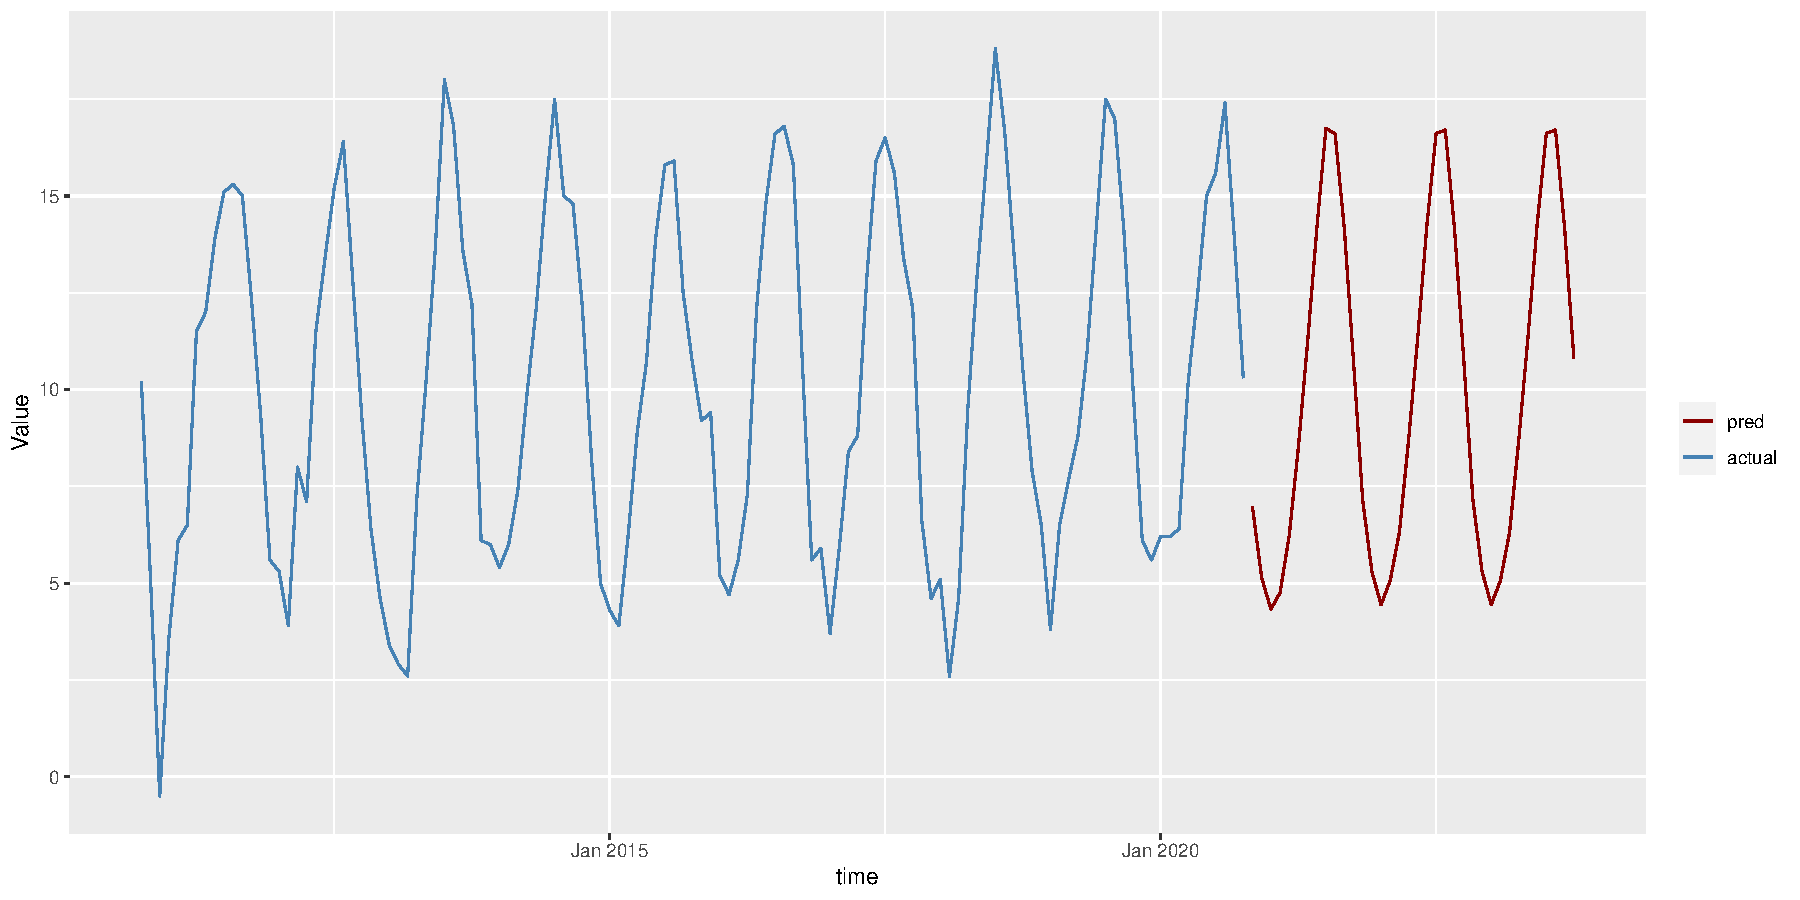
\includegraphics{ST422_files/figure-latex/unnamed-chunk-54-1.pdf}
\caption{sVARMA 2 years forecast on Mean Temperature}
\end{figure}

From 2 years forecast plot, it is shown that the predicted values (2
years) of sVARMA model mimics the historic trend well. In addition to
this, the predicted values of sVARMA are further examined below by
comparing with the 2 months forecast of SARIMA which was identified in
the earlier section.

\newpage

\begin{figure}
\centering
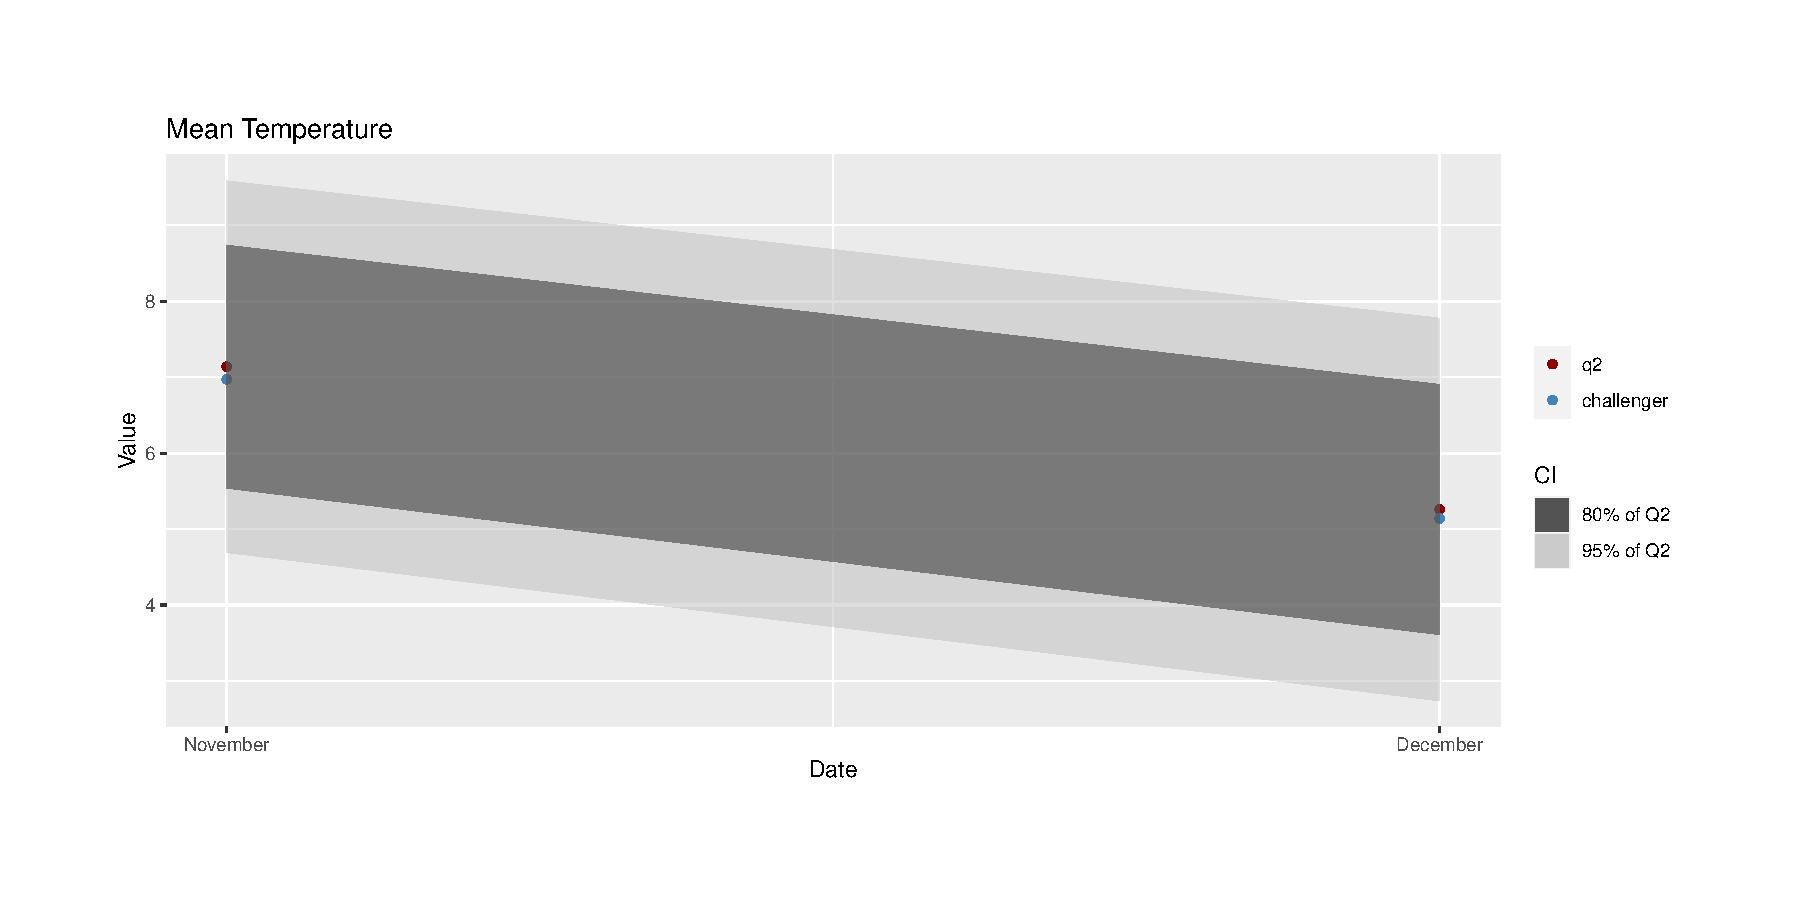
\includegraphics{ST422_files/figure-latex/unnamed-chunk-55-1.pdf}
\caption{Mean Temperature: Q2 (SARIMA) vs Q4 (challenger, sVARMA)}
\end{figure}

Based on 2 Months forecast of Mean Temperature of Question 2 (Q2) and
Question 4 (Q4) models, the extra 2 months of foretasted points
retrieved from Q4 fall within the C.I (incl.~95\% and 80\%) of Q2
forecasts and the divergence between Q2 and Q4 forecasts is obsereved to
be immaterial.

\newpage
\newpage

\hypertarget{appendix-all-code-for-this-report}{%
\section{Appendix: All code for this
report}\label{appendix-all-code-for-this-report}}

\begin{Shaded}
\begin{Highlighting}[]
\CommentTok{# Library Setup}
\KeywordTok{library}\NormalTok{(zoo)}
\KeywordTok{library}\NormalTok{(astsa)}
\KeywordTok{library}\NormalTok{(forecast)}
\KeywordTok{library}\NormalTok{(ggplot2)}
\KeywordTok{library}\NormalTok{(ggfortify)}
\KeywordTok{library}\NormalTok{(tseries)}
\KeywordTok{library}\NormalTok{(tidyverse)}
\KeywordTok{library}\NormalTok{(tsutils)}
\KeywordTok{library}\NormalTok{(MTS)}
\KeywordTok{library}\NormalTok{(knitr)}

\CommentTok{# Data retrieved from Git-hub repository.}
\NormalTok{df_path =}\StringTok{ "https://raw.githubusercontent.com/Anko-Jipsa/statistics/master/ST422/"}

\CommentTok{# Mean Temperature}
\NormalTok{mt_df <-}\StringTok{ }\KeywordTok{read.csv}\NormalTok{(}
  \KeywordTok{paste}\NormalTok{(df_path, }\StringTok{"/MonthlyMeanTemp.csv"}\NormalTok{, }\DataTypeTok{sep =} \StringTok{""}\NormalTok{),}
  \DataTypeTok{header =} \OtherTok{TRUE}\NormalTok{,}
  \DataTypeTok{row.names =} \StringTok{"year"}
\NormalTok{)}

\CommentTok{# Sunshine}
\NormalTok{ss_df <-}\StringTok{ }\KeywordTok{read.csv}\NormalTok{(}
  \KeywordTok{paste}\NormalTok{(df_path, }\StringTok{"/MonthlySunshine.csv"}\NormalTok{, }\DataTypeTok{sep =} \StringTok{""}\NormalTok{),}
  \DataTypeTok{header =} \OtherTok{TRUE}\NormalTok{,}
  \DataTypeTok{row.names =} \StringTok{"year"}
\NormalTok{)}

\CommentTok{# Rainfall}
\NormalTok{rf_df <-}\StringTok{ }\KeywordTok{read.csv}\NormalTok{(}
  \KeywordTok{paste}\NormalTok{(df_path, }\StringTok{"/MonthlyRainfall.csv"}\NormalTok{, }\DataTypeTok{sep =} \StringTok{""}\NormalTok{),}
  \DataTypeTok{header =} \OtherTok{TRUE}\NormalTok{,}
  \DataTypeTok{row.names =} \StringTok{"year"}
\NormalTok{)}

\CommentTok{# Vectorisation of CSV imported dataset}
\NormalTok{vectorised_ts =}\StringTok{ }\ControlFlowTok{function}\NormalTok{(df) \{}
  \CommentTok{#' Generate a time-series vector, ignoring aggregated level data.}
  \CommentTok{#'}
  \CommentTok{#' @param df (data.frame): A data-frame that contains the time-series vector.}
  \CommentTok{#' @return A time-series vector without aggregated level data.}
  
\NormalTok{  start_year =}\StringTok{ }\KeywordTok{as.numeric}\NormalTok{(}\KeywordTok{row.names}\NormalTok{(df)[}\DecValTok{1}\NormalTok{])}
  
  
\NormalTok{  vector_df =}\StringTok{ }\KeywordTok{as.numeric}\NormalTok{(}\KeywordTok{t}\NormalTok{(df[, }\DecValTok{1}\OperatorTok{:}\DecValTok{12}\NormalTok{])) }\CommentTok{# Flattening 2d data.}
\NormalTok{  vector_df =}\StringTok{ }\KeywordTok{na.omit}\NormalTok{(vector_df) }\CommentTok{# Drop null values.}
\NormalTok{  vector_ts =}\StringTok{ }\KeywordTok{ts}\NormalTok{(vector_df,}
                 \DataTypeTok{start =} \KeywordTok{c}\NormalTok{(start_year, }\DecValTok{1}\NormalTok{),}
                 \DataTypeTok{frequency =} \DecValTok{12}\NormalTok{) }\CommentTok{# Assigning time-series.}
  \KeywordTok{return}\NormalTok{(vector_ts)}
\NormalTok{\}}

\CommentTok{# Transforming data}
\NormalTok{mt_ts =}\StringTok{ }\KeywordTok{vectorised_ts}\NormalTok{(mt_df)}
\NormalTok{ss_ts =}\StringTok{ }\KeywordTok{vectorised_ts}\NormalTok{(ss_df)}
\NormalTok{rf_ts =}\StringTok{ }\KeywordTok{vectorised_ts}\NormalTok{(rf_df)}

\CommentTok{####################Q1 & Q2######################}
\CommentTok{# Preliminary analysis for identification of Time-series model}
\NormalTok{prelim_analysis =}\StringTok{ }\ControlFlowTok{function}\NormalTok{(ts_v,}
                           \DataTypeTok{title =} \OtherTok{NULL}\NormalTok{,}
                           \DataTypeTok{start_year =} \OtherTok{NULL}\NormalTok{,}
                           \DataTypeTok{start_month =} \OtherTok{NULL}\NormalTok{) \{}
  \CommentTok{#' Preliminary analysis for Time Series.}
  \CommentTok{#' }
  \CommentTok{#' @description}
  \CommentTok{#' Generate time-series analysis graphs:}
  \CommentTok{#' 1. Time Series plot (General visualisation)}
  \CommentTok{#' 2. Box plot (Seasonality & volatility assessment)}
  \CommentTok{#' 3. Seasonal Plot (Deeper insight on pattern)}
  \CommentTok{#' 4. Decomposition plot (Assess trend, seasonality and remainder)}
  \CommentTok{#'}
  \CommentTok{#' @param ts_v (vector): A Time Series vector.}
  \CommentTok{#' @param title (str): Title of the plot. Defaults to NULL.}
  \CommentTok{#' @param start_year (int): A starting year of analysis. Defaults to NULL.}
  \CommentTok{#' @param start_month (int): A starting month of analysis. Defaults to NULL.}
  
  \ControlFlowTok{if}\NormalTok{ (}\OperatorTok{!}\KeywordTok{is.null}\NormalTok{(start)) \{}
\NormalTok{    ts_v =}\StringTok{ }\KeywordTok{window}\NormalTok{(ts_v,}
                \DataTypeTok{start =} \KeywordTok{c}\NormalTok{(start_year, start_month),}
                \DataTypeTok{end =} \KeywordTok{c}\NormalTok{(}\DecValTok{2020}\NormalTok{, }\DecValTok{12}\NormalTok{))}
\NormalTok{  \}}
  \KeywordTok{layout}\NormalTok{(}\KeywordTok{matrix}\NormalTok{(}\KeywordTok{c}\NormalTok{(}\DecValTok{1}\NormalTok{,}\DecValTok{1}\NormalTok{,}\DecValTok{2}\NormalTok{,}\DecValTok{3}\NormalTok{), }\DecValTok{2}\NormalTok{, }\DecValTok{2}\NormalTok{, }\DataTypeTok{byrow =} \OtherTok{TRUE}\NormalTok{))}
  \KeywordTok{plot.ts}\NormalTok{(ts_v,}
          \DataTypeTok{ylab =} \StringTok{"Value"}\NormalTok{,}
          \DataTypeTok{xlab =} \StringTok{"Date"}\NormalTok{,}
          \DataTypeTok{main =} \KeywordTok{paste}\NormalTok{(title, }\StringTok{"TS plot"}\NormalTok{, }\DataTypeTok{sep =} \StringTok{" "}\NormalTok{))}
  \KeywordTok{boxplot}\NormalTok{(ts_v }\OperatorTok{~}\StringTok{ }\KeywordTok{cycle}\NormalTok{(ts_v),}
          \DataTypeTok{ylab =} \StringTok{"Value"}\NormalTok{,}
          \DataTypeTok{xlab =} \StringTok{"Month"}\NormalTok{,}
          \DataTypeTok{main =} \StringTok{"Box Plot"}\NormalTok{)}
  \KeywordTok{seasonplot}\NormalTok{(ts_v, }
             \DataTypeTok{year.labels =} \OtherTok{TRUE}\NormalTok{, }
             \DataTypeTok{col =} \DecValTok{1}\OperatorTok{:}\DecValTok{13}\NormalTok{,}
           \DataTypeTok{main =} \StringTok{"Seasonal Plot"}\NormalTok{, }
           \DataTypeTok{ylab=} \StringTok{"Value"}\NormalTok{)}
\NormalTok{\}}

\CommentTok{# Decomposition analysis required for Time-series model identification}
\NormalTok{decomp_analysis =}\StringTok{ }\ControlFlowTok{function}\NormalTok{(ts_v,}
                           \DataTypeTok{title =} \OtherTok{NULL}\NormalTok{,}
                           \DataTypeTok{start_year =} \OtherTok{NULL}\NormalTok{,}
                           \DataTypeTok{start_month =} \OtherTok{NULL}\NormalTok{) \{}
  \CommentTok{#' Decomposition analysis for Time Series.}
  \CommentTok{#' }
  \CommentTok{#' @description}
  \CommentTok{#' Generate time-series analysis graphs:}
  \CommentTok{#' 1. Decomposition plot (Assess trend, seasonality and remainder)}
  \CommentTok{#'}
  \CommentTok{#' @param ts_v (vector): A Time Series vector.}
  \CommentTok{#' @param title (str): Title of the plot. Defaults to NULL.}
  \CommentTok{#' @param start_year (int): A starting year of analysis. Defaults to NULL.}
  \CommentTok{#' @param start_month (int): A starting month of analysis. Defaults to NULL.}
  
  \ControlFlowTok{if}\NormalTok{ (}\OperatorTok{!}\KeywordTok{is.null}\NormalTok{(start)) \{}
\NormalTok{    ts_v =}\StringTok{ }\KeywordTok{window}\NormalTok{(ts_v,}
                \DataTypeTok{start =} \KeywordTok{c}\NormalTok{(start_year, start_month),}
                \DataTypeTok{end =} \KeywordTok{c}\NormalTok{(}\DecValTok{2020}\NormalTok{, }\DecValTok{12}\NormalTok{))}
\NormalTok{  \}}
  
\NormalTok{  decomp <-}\StringTok{ }\KeywordTok{stl}\NormalTok{(ts_v, }\DataTypeTok{s.window =} \StringTok{'periodic'}\NormalTok{)}
  \KeywordTok{autoplot}\NormalTok{(decomp) }\OperatorTok{+}\StringTok{  }\KeywordTok{ggtitle}\NormalTok{(}\StringTok{"Remainder"}\NormalTok{)}
\NormalTok{\}}

\CommentTok{# Entire dataset}
\KeywordTok{prelim_analysis}\NormalTok{(ss_ts, }\StringTok{"Sunshine"}\NormalTok{)}
\KeywordTok{decomp_analysis}\NormalTok{(ss_ts, }\StringTok{"Sunshine"}\NormalTok{)}

\CommentTok{# Dataset from 2000}
\KeywordTok{prelim_analysis}\NormalTok{(ss_ts, }\StringTok{"Sunshine"}\NormalTok{, }\DecValTok{2000}\NormalTok{, }\DecValTok{1}\NormalTok{)}
\KeywordTok{decomp_analysis}\NormalTok{(ss_ts, }\StringTok{"Sunshine"}\NormalTok{, }\DecValTok{2000}\NormalTok{, }\DecValTok{1}\NormalTok{)}

\CommentTok{# Time-series analysis required for model identification}
\NormalTok{ts_analysis =}\StringTok{ }\ControlFlowTok{function}\NormalTok{(ts_v,}
                       \DataTypeTok{title =} \OtherTok{NULL}\NormalTok{,}
                       \DataTypeTok{start_year =} \OtherTok{NULL}\NormalTok{,}
                       \DataTypeTok{start_month =} \OtherTok{NULL}\NormalTok{)\{}
  \CommentTok{#' ACF & PACF analysis for Time Series.}
  \CommentTok{#' }
  \CommentTok{#' @description}
  \CommentTok{#' Generate time-series analysis graphs:}
  \CommentTok{#' 1. ACF}
  \CommentTok{#' 2. PACF}
  \CommentTok{#' 3. Seasonal Plot (Deeper insight on pattern)}
  \CommentTok{#' 4. Decomposition plot (Assess trend, seasonality and remainder)}
  \CommentTok{#'}
  \CommentTok{#' @param ts_v (vector): A Time Series vector.}
  \CommentTok{#' @param title (str): Title of the plot. Defaults to NULL.}
  \CommentTok{#' @param start_year (int): A starting year of analysis. Defaults to NULL.}
  \CommentTok{#' @param start_month (int): A starting month of analysis. Defaults to NULL.}
  
  
  \KeywordTok{acf2}\NormalTok{(ts_v, }\DataTypeTok{main=}\NormalTok{title)}
  
  
  \KeywordTok{adf.test}\NormalTok{(ts_v, }\DataTypeTok{k=}\DecValTok{12}\NormalTok{)}
\NormalTok{\}}

\KeywordTok{ts_analysis}\NormalTok{(ss_ts, }\StringTok{"Sunshine"}\NormalTok{)}

\CommentTok{# Seasonally differenced time-series}
\NormalTok{d12_ss_ts =}\StringTok{ }\KeywordTok{diff}\NormalTok{(ss_ts, }\DataTypeTok{lag =} \DecValTok{12}\NormalTok{)}
\KeywordTok{ts_analysis}\NormalTok{(d12_ss_ts)}

\CommentTok{# Grid-search method for model exploration}
\NormalTok{grid_search_sarima =}\StringTok{ }\ControlFlowTok{function}\NormalTok{(ts_v, non_seasonal_pqd, seasonal_pqd) \{}
  \CommentTok{#' Grid-search function to find the multiplicative seasonal ARIMA model with the best fit.}
  \CommentTok{#'}
  \CommentTok{#' @description}
  \CommentTok{#' Exhaustive approach of derive multiplicative seasonal ARIMA model.}
  \CommentTok{#' Iterate through each P, Q terms of non-seasonal and seasonal components. (D is fixed.)}
  \CommentTok{#'}
  \CommentTok{#' @param ts_v (vector): A Time Series vector.}
  \CommentTok{#' @param non_seasonal_pqd (vector): Initial P, Q, D elements for non-seasonal component.}
  \CommentTok{#' @param non_seasonal_pqd (vector): Initial P, Q, D elements for seasonal component.}
  
\NormalTok{  cross_non_pqd =}\StringTok{ }\KeywordTok{expand.grid}\NormalTok{(}\KeywordTok{seq}\NormalTok{(}\KeywordTok{max}\NormalTok{(non_seasonal_pqd[}\DecValTok{1}\NormalTok{]}\OperatorTok{-}\DecValTok{1}\NormalTok{, }\DecValTok{0}\NormalTok{), non_seasonal_pqd[}\DecValTok{1}\NormalTok{] }\OperatorTok{+}\StringTok{ }\DecValTok{1}\NormalTok{),}
\NormalTok{                              non_seasonal_pqd[}\DecValTok{2}\NormalTok{],}
                              \KeywordTok{seq}\NormalTok{(}\KeywordTok{max}\NormalTok{(non_seasonal_pqd[}\DecValTok{3}\NormalTok{]}\OperatorTok{-}\DecValTok{1}\NormalTok{, }\DecValTok{0}\NormalTok{), non_seasonal_pqd[}\DecValTok{3}\NormalTok{] }\OperatorTok{+}\StringTok{ }\DecValTok{1}\NormalTok{))}
  
\NormalTok{  cross_pqd =}\StringTok{ }\KeywordTok{expand.grid}\NormalTok{(}\KeywordTok{seq}\NormalTok{(}\KeywordTok{max}\NormalTok{(seasonal_pqd[}\DecValTok{1}\NormalTok{]}\OperatorTok{-}\DecValTok{1}\NormalTok{, }\DecValTok{0}\NormalTok{), seasonal_pqd[}\DecValTok{1}\NormalTok{] }\OperatorTok{+}\StringTok{ }\DecValTok{1}\NormalTok{),}
\NormalTok{                          seasonal_pqd[}\DecValTok{2}\NormalTok{],}
                          \KeywordTok{seq}\NormalTok{(}\KeywordTok{max}\NormalTok{(seasonal_pqd[}\DecValTok{3}\NormalTok{]}\OperatorTok{-}\DecValTok{1}\NormalTok{, }\DecValTok{0}\NormalTok{), seasonal_pqd[}\DecValTok{3}\NormalTok{] }\OperatorTok{+}\StringTok{ }\DecValTok{1}\NormalTok{))}
  
  \CommentTok{# Empty model rank table}
\NormalTok{  mod_fit =}\StringTok{ }\KeywordTok{data.frame}\NormalTok{(}\DataTypeTok{AIC =} \KeywordTok{numeric}\NormalTok{(}\DecValTok{0}\NormalTok{), }
                       \DataTypeTok{BIC =} \KeywordTok{numeric}\NormalTok{(}\DecValTok{0}\NormalTok{),}
                       \DataTypeTok{NON_SEASONAL =} \KeywordTok{numeric}\NormalTok{(}\DecValTok{0}\NormalTok{),}
                       \DataTypeTok{SEASONAL=} \KeywordTok{numeric}\NormalTok{(}\DecValTok{0}\NormalTok{))}
\NormalTok{  count =}\StringTok{ }\DecValTok{1}
  \ControlFlowTok{for}\NormalTok{ (i }\ControlFlowTok{in} \DecValTok{1}\OperatorTok{:}\KeywordTok{dim}\NormalTok{(cross_non_pqd)[}\DecValTok{1}\NormalTok{])\{}
    \ControlFlowTok{for}\NormalTok{ (j }\ControlFlowTok{in} \DecValTok{1}\OperatorTok{:}\KeywordTok{dim}\NormalTok{(cross_pqd)[}\DecValTok{1}\NormalTok{])\{}
\NormalTok{      skip_to_next <-}\StringTok{ }\OtherTok{FALSE}
      
      \CommentTok{# Status update prints}
      \KeywordTok{print}\NormalTok{(}\StringTok{"************************"}\NormalTok{)}
      \KeywordTok{print}\NormalTok{(}\KeywordTok{paste}\NormalTok{(}\StringTok{"Iteration: "}\NormalTok{, count, }\DataTypeTok{sep =} \StringTok{""}\NormalTok{))}
      \KeywordTok{print}\NormalTok{(}\KeywordTok{paste}\NormalTok{(}\StringTok{"Non-Seasonal: "}\NormalTok{, cross_pqd[j,], }\DataTypeTok{sep =} \StringTok{""}\NormalTok{))}
      \KeywordTok{print}\NormalTok{(}\KeywordTok{paste}\NormalTok{(}\StringTok{"Seasonal: "}\NormalTok{,cross_non_pqd[i,], }\DataTypeTok{sep =} \StringTok{""}\NormalTok{)) }

      \CommentTok{# Error catcher for ARIMA fitting (In case of optimisation error)}
\NormalTok{      mod =}\StringTok{ }\KeywordTok{tryCatch}\NormalTok{(}\KeywordTok{Arima}\NormalTok{(ts_v,}
                           \DataTypeTok{order =} \KeywordTok{as.numeric}\NormalTok{(cross_non_pqd[i,]),}
                           \DataTypeTok{seasonal =} \KeywordTok{list}\NormalTok{(}\DataTypeTok{order =} \KeywordTok{as.numeric}\NormalTok{(cross_pqd[j,]), }\DataTypeTok{period =} \DecValTok{12}\NormalTok{)), }
                     \DataTypeTok{error =} \ControlFlowTok{function}\NormalTok{(e) \{ skip_to_next <<-}\StringTok{ }\OtherTok{TRUE}\NormalTok{\})}
      \ControlFlowTok{if}\NormalTok{(skip_to_next) \{ }\ControlFlowTok{next}\NormalTok{ \}}
      
      \CommentTok{# Table filling}
\NormalTok{      mod_fit[count, ] =}\StringTok{ }\KeywordTok{c}\NormalTok{(mod}\OperatorTok{$}\NormalTok{aic, }
\NormalTok{                           mod}\OperatorTok{$}\NormalTok{bic,}
                           \KeywordTok{paste}\NormalTok{(}\KeywordTok{as.character}\NormalTok{(cross_non_pqd[i,]), }\DataTypeTok{collapse=}\StringTok{","}\NormalTok{), }
                           \KeywordTok{paste}\NormalTok{(}\KeywordTok{as.character}\NormalTok{(cross_pqd[j,]), }\DataTypeTok{collapse=}\StringTok{","}\NormalTok{))}
      
\NormalTok{      count =}\StringTok{ }\NormalTok{count }\OperatorTok{+}\StringTok{ }\DecValTok{1}
\NormalTok{    \}}
\NormalTok{  \}}
  \CommentTok{# Reordering}
\NormalTok{  mod_fit =}\StringTok{ }\NormalTok{mod_fit }\OperatorTok\StringTok{ }\KeywordTok{arrange}\NormalTok{(AIC)}
  \KeywordTok{return}\NormalTok{(mod_fit)}
\NormalTok{\}}

\CommentTok{# Grid-search}
\NormalTok{grid_ss =}\StringTok{ }\KeywordTok{grid_search_sarima}\NormalTok{(ss_ts, }
                            \KeywordTok{c}\NormalTok{(}\DecValTok{0}\NormalTok{,}\DecValTok{0}\NormalTok{,}\DecValTok{2}\NormalTok{), }
                            \KeywordTok{c}\NormalTok{(}\DecValTok{0}\NormalTok{,}\DecValTok{1}\NormalTok{,}\DecValTok{1}\NormalTok{))}
\NormalTok{opt_non_seasonal =}\StringTok{ }\KeywordTok{as.numeric}\NormalTok{(}\KeywordTok{unlist}\NormalTok{(}\KeywordTok{strsplit}\NormalTok{(grid_ss[}\DecValTok{1}\NormalTok{,}\DecValTok{3}\NormalTok{], }\StringTok{"}\CharTok{\textbackslash{}\textbackslash{}}\StringTok{,"}\NormalTok{))) }\CommentTok{# Optimal non-seasonal P, D, Q parameters}
\NormalTok{opt_seasonal =}\StringTok{ }\KeywordTok{as.numeric}\NormalTok{(}\KeywordTok{unlist}\NormalTok{(}\KeywordTok{strsplit}\NormalTok{(grid_ss[}\DecValTok{1}\NormalTok{,}\DecValTok{4}\NormalTok{], }\StringTok{"}\CharTok{\textbackslash{}\textbackslash{}}\StringTok{,"}\NormalTok{))) }\CommentTok{# Optimal seasonal P, D, Q parameters}

\CommentTok{# Model fitting}
\NormalTok{best_guess_ss =}\StringTok{ }\KeywordTok{Arima}\NormalTok{(ss_ts,}
                   \DataTypeTok{order=}\KeywordTok{c}\NormalTok{(}\DecValTok{0}\NormalTok{,}\DecValTok{0}\NormalTok{,}\DecValTok{2}\NormalTok{),}
                   \DataTypeTok{seasonal=}\KeywordTok{list}\NormalTok{(}\DataTypeTok{order=}\KeywordTok{c}\NormalTok{(}\DecValTok{0}\NormalTok{,}\DecValTok{1}\NormalTok{,}\DecValTok{1}\NormalTok{), }\DataTypeTok{period=}\DecValTok{12}\NormalTok{))}

\NormalTok{optimal_ss =}\StringTok{ }\KeywordTok{Arima}\NormalTok{(ss_ts,}
                   \DataTypeTok{order=}\NormalTok{opt_non_seasonal,}
                   \DataTypeTok{seasonal=}\KeywordTok{list}\NormalTok{(}\DataTypeTok{order=}\NormalTok{opt_seasonal, }\DataTypeTok{period=}\DecValTok{12}\NormalTok{))}

\NormalTok{auto_arima_ss =}\StringTok{ }\KeywordTok{auto.arima}\NormalTok{(ss_ts)}

\CommentTok{# Model comparison}
\NormalTok{best_guess_ss }\CommentTok{# Best guess}
\NormalTok{optimal_ss }\CommentTok{# Grid-search}
\NormalTok{auto_arima_ss }\CommentTok{# auto.arima}

\CommentTok{# Residual analysis}
\KeywordTok{checkresiduals}\NormalTok{(best_guess_ss)}
\KeywordTok{tsdiag}\NormalTok{(best_guess_ss)}

\CommentTok{# Custom ggplot function}
\NormalTok{gg_forecast =}\StringTok{ }\ControlFlowTok{function}\NormalTok{(model_output, n_forecast, include, title)\{}
  \CommentTok{#' Custom function for clear ggplot of forecast object.}
  \CommentTok{#'}
  \CommentTok{#' @param model_output (obj): a time series or time series model for which forecasts are required}
  \CommentTok{#' @param n_forecast (int): Number of periods for forecasting}
  \CommentTok{#' @param include (int): Number of periods for previous actuals }
  \CommentTok{#' @param title (str): Title of the plot.}
  \CommentTok{#'}
  
  \CommentTok{# Actual & Forecasts}
\NormalTok{  forecast_obj =}\StringTok{ }\KeywordTok{forecast}\NormalTok{(model_output, n_forecast)}
\NormalTok{  actuals =}\StringTok{ }\KeywordTok{tail}\NormalTok{(forecast_obj}\OperatorTok{$}\NormalTok{x, include)}
\NormalTok{  predicted =}\StringTok{ }\NormalTok{forecast_obj}\OperatorTok{$}\NormalTok{mean}
  
  \CommentTok{# Date}
\NormalTok{  date_window =}\StringTok{ }\KeywordTok{c}\NormalTok{(}\KeywordTok{as.Date}\NormalTok{(actuals), }\KeywordTok{as.Date}\NormalTok{(predicted))}
  
  \CommentTok{# Combined data.frame}
\NormalTok{  output =}\StringTok{ }\KeywordTok{data.frame}\NormalTok{(}\DataTypeTok{time =}\NormalTok{ date_window,}
                      \DataTypeTok{actual =} \KeywordTok{c}\NormalTok{(actuals, }\KeywordTok{rep}\NormalTok{(}\OtherTok{NA}\NormalTok{,}\KeywordTok{length}\NormalTok{(predicted))),}
                      \DataTypeTok{pred =} \KeywordTok{c}\NormalTok{(}\KeywordTok{rep}\NormalTok{(}\OtherTok{NA}\NormalTok{,}\KeywordTok{length}\NormalTok{(actuals)), predicted),}
                      \DataTypeTok{low_95 =} \KeywordTok{c}\NormalTok{(}\KeywordTok{rep}\NormalTok{(}\OtherTok{NA}\NormalTok{,}\KeywordTok{length}\NormalTok{(actuals)), forecast_obj}\OperatorTok{$}\NormalTok{lower[,}\DecValTok{2}\NormalTok{]),}
                      \DataTypeTok{up_95 =} \KeywordTok{c}\NormalTok{(}\KeywordTok{rep}\NormalTok{(}\OtherTok{NA}\NormalTok{,}\KeywordTok{length}\NormalTok{(actuals)), forecast_obj}\OperatorTok{$}\NormalTok{upper[,}\DecValTok{2}\NormalTok{]),}
                      \DataTypeTok{low_80 =} \KeywordTok{c}\NormalTok{(}\KeywordTok{rep}\NormalTok{(}\OtherTok{NA}\NormalTok{,}\KeywordTok{length}\NormalTok{(actuals)), forecast_obj}\OperatorTok{$}\NormalTok{lower[,}\DecValTok{1}\NormalTok{]),}
                      \DataTypeTok{up_80 =} \KeywordTok{c}\NormalTok{(}\KeywordTok{rep}\NormalTok{(}\OtherTok{NA}\NormalTok{,}\KeywordTok{length}\NormalTok{(actuals)), forecast_obj}\OperatorTok{$}\NormalTok{upper[,}\DecValTok{1}\NormalTok{])}
\NormalTok{                      )}
  
  \CommentTok{# ggplot}
\NormalTok{  p =}\StringTok{ }\KeywordTok{ggplot}\NormalTok{(output, }\KeywordTok{aes}\NormalTok{(}\DataTypeTok{x=}\NormalTok{time), }\DataTypeTok{na.rm=}\OtherTok{TRUE}\NormalTok{) }\OperatorTok{+}\StringTok{  }\KeywordTok{geom_line}\NormalTok{(}\KeywordTok{aes}\NormalTok{(}\DataTypeTok{y=}\NormalTok{actual, }\DataTypeTok{color=}\StringTok{"actual"}\NormalTok{), }\DataTypeTok{na.rm=}\OtherTok{TRUE}\NormalTok{)}
  \CommentTok{# Convert to scatter plots for forecast periods less than 10}
    \ControlFlowTok{if}\NormalTok{ (n_forecast}\OperatorTok{<}\DecValTok{10}\NormalTok{)\{}
\NormalTok{      p =}\StringTok{ }\NormalTok{p }\OperatorTok{+}\StringTok{ }\KeywordTok{geom_point}\NormalTok{(}\KeywordTok{aes}\NormalTok{(}\DataTypeTok{y=}\NormalTok{pred, }\DataTypeTok{color=}\StringTok{"pred"}\NormalTok{), }\DataTypeTok{na.rm=}\OtherTok{TRUE}\NormalTok{)}
\NormalTok{      \} }\ControlFlowTok{else}\NormalTok{ \{}
\NormalTok{        p =}\StringTok{ }\NormalTok{p }\OperatorTok{+}\StringTok{ }\KeywordTok{geom_line}\NormalTok{(}\KeywordTok{aes}\NormalTok{(}\DataTypeTok{y=}\NormalTok{pred, }\DataTypeTok{color=}\StringTok{"pred"}\NormalTok{), }\DataTypeTok{na.rm=}\OtherTok{TRUE}\NormalTok{)}
\NormalTok{      \}}
  
  \CommentTok{# Confidence interval }
\NormalTok{  p =}\StringTok{ }\NormalTok{p }\OperatorTok{+}
\StringTok{    }\KeywordTok{geom_ribbon}\NormalTok{(}\KeywordTok{aes}\NormalTok{(}\DataTypeTok{ymin=}\NormalTok{low_}\DecValTok{95}\NormalTok{, }\DataTypeTok{ymax=}\NormalTok{up_}\DecValTok{95}\NormalTok{, }\DataTypeTok{fill=}\StringTok{"95% CI"}\NormalTok{),}\DataTypeTok{linetype=}\DecValTok{2}\NormalTok{, }\DataTypeTok{alpha=}\FloatTok{0.5}\NormalTok{) }\OperatorTok{+}
\StringTok{    }\KeywordTok{geom_ribbon}\NormalTok{(}\KeywordTok{aes}\NormalTok{(}\DataTypeTok{ymin=}\NormalTok{low_}\DecValTok{80}\NormalTok{, }\DataTypeTok{ymax=}\NormalTok{up_}\DecValTok{80}\NormalTok{, }\DataTypeTok{fill=}\StringTok{"80% CI"}\NormalTok{), }\DataTypeTok{linetype=}\DecValTok{2}\NormalTok{, }\DataTypeTok{alpha=}\FloatTok{0.5}\NormalTok{)}
  
  \CommentTok{# Further aesthetics}
\NormalTok{  p =}\StringTok{ }\NormalTok{p }\OperatorTok{+}
\StringTok{    }\KeywordTok{scale_colour_manual}\NormalTok{(}\StringTok{""}\NormalTok{, }
                        \DataTypeTok{breaks =} \KeywordTok{c}\NormalTok{(}\StringTok{"pred"}\NormalTok{, }\StringTok{"actual"}\NormalTok{),}
                        \DataTypeTok{values =} \KeywordTok{c}\NormalTok{(}\StringTok{"darkred"}\NormalTok{, }\StringTok{"steelblue"}\NormalTok{)) }\OperatorTok{+}\StringTok{ }
\StringTok{    }\KeywordTok{scale_fill_manual}\NormalTok{(}\DataTypeTok{values=}\KeywordTok{c}\NormalTok{(}\StringTok{"grey12"}\NormalTok{, }\StringTok{"grey"}\NormalTok{), }\DataTypeTok{name=}\StringTok{"fill"}\NormalTok{) }\OperatorTok{+}\StringTok{ }
\StringTok{    }\KeywordTok{ylab}\NormalTok{(}\StringTok{"Value"}\NormalTok{) }\OperatorTok{+}\StringTok{ }\KeywordTok{xlab}\NormalTok{(}\StringTok{"Date"}\NormalTok{) }\OperatorTok{+}\StringTok{ }\KeywordTok{ggtitle}\NormalTok{(title)}
  
  \KeywordTok{return}\NormalTok{(p)}
\NormalTok{\}}

\CommentTok{# Forecasting}
\KeywordTok{gg_forecast}\NormalTok{(best_guess_ss, }\DataTypeTok{n_forecast=}\DecValTok{2}\NormalTok{, }\DataTypeTok{include=}\DecValTok{12}\NormalTok{, }\DataTypeTok{title=}\StringTok{"2 Months forecast plot of Sunshine"}\NormalTok{)}
\KeywordTok{forecast}\NormalTok{(best_guess_ss, }\DecValTok{2}\NormalTok{)}
\KeywordTok{gg_forecast}\NormalTok{(best_guess_ss, }\DataTypeTok{n_forecast=}\DecValTok{24}\NormalTok{, }\DataTypeTok{include=}\DecValTok{120}\NormalTok{, }\DataTypeTok{title=}\StringTok{"2 years forecast plot of Sunshine"}\NormalTok{)}

\CommentTok{# Description of the following codes is identical to the above case}
\KeywordTok{prelim_analysis}\NormalTok{(rf_ts, }\StringTok{"Rainfall"}\NormalTok{)}
\KeywordTok{decomp_analysis}\NormalTok{(rf_ts, }\StringTok{"Rainfall"}\NormalTok{)}
\KeywordTok{prelim_analysis}\NormalTok{(rf_ts, }\StringTok{"Rainfall"}\NormalTok{, }\DecValTok{2010}\NormalTok{, }\DecValTok{1}\NormalTok{)}
\KeywordTok{decomp_analysis}\NormalTok{(rf_ts, }\StringTok{"Rainfall"}\NormalTok{, }\DecValTok{2000}\NormalTok{, }\DecValTok{1}\NormalTok{)}

\CommentTok{# Time-series analysis}
\KeywordTok{ts_analysis}\NormalTok{(rf_ts, }\StringTok{"Rainfall"}\NormalTok{)}

\CommentTok{# Seasonally differenced Time-series analysis}
\NormalTok{d12_rf_ts =}\StringTok{ }\KeywordTok{diff}\NormalTok{(rf_ts, }\DataTypeTok{lag =} \DecValTok{12}\NormalTok{)}
\KeywordTok{ts_analysis}\NormalTok{(d12_rf_ts)}

\CommentTok{# Grid-search}
\NormalTok{grid_rf =}\StringTok{ }\KeywordTok{grid_search_sarima}\NormalTok{(rf_ts, }
                            \KeywordTok{c}\NormalTok{(}\DecValTok{1}\NormalTok{,}\DecValTok{0}\NormalTok{,}\DecValTok{1}\NormalTok{), }
                            \KeywordTok{c}\NormalTok{(}\DecValTok{0}\NormalTok{,}\DecValTok{1}\NormalTok{,}\DecValTok{1}\NormalTok{))}
\NormalTok{opt_non_seasonal =}\StringTok{ }\KeywordTok{as.numeric}\NormalTok{(}\KeywordTok{unlist}\NormalTok{(}\KeywordTok{strsplit}\NormalTok{(grid_rf[}\DecValTok{1}\NormalTok{,}\DecValTok{3}\NormalTok{], }\StringTok{"}\CharTok{\textbackslash{}\textbackslash{}}\StringTok{,"}\NormalTok{))) }\CommentTok{# Optimal non-seasonal P, D, Q parameters}
\NormalTok{opt_seasonal =}\StringTok{ }\KeywordTok{as.numeric}\NormalTok{(}\KeywordTok{unlist}\NormalTok{(}\KeywordTok{strsplit}\NormalTok{(grid_rf[}\DecValTok{1}\NormalTok{,}\DecValTok{4}\NormalTok{], }\StringTok{"}\CharTok{\textbackslash{}\textbackslash{}}\StringTok{,"}\NormalTok{))) }\CommentTok{# Optimal seasonal P, D, Q parameters}

\CommentTok{# Comparison}
\NormalTok{best_guess_rf =}\StringTok{ }\KeywordTok{Arima}\NormalTok{(rf_ts,}
                   \DataTypeTok{order=}\KeywordTok{c}\NormalTok{(}\DecValTok{1}\NormalTok{,}\DecValTok{0}\NormalTok{,}\DecValTok{1}\NormalTok{),}
                   \DataTypeTok{seasonal=}\KeywordTok{list}\NormalTok{(}\DataTypeTok{order=}\KeywordTok{c}\NormalTok{(}\DecValTok{0}\NormalTok{,}\DecValTok{1}\NormalTok{,}\DecValTok{1}\NormalTok{), }\DataTypeTok{period=}\DecValTok{12}\NormalTok{))}

\NormalTok{optimal_rf =}\StringTok{ }\KeywordTok{Arima}\NormalTok{(rf_ts,}
                   \DataTypeTok{order=}\NormalTok{opt_non_seasonal,}
                   \DataTypeTok{seasonal=}\KeywordTok{list}\NormalTok{(}\DataTypeTok{order=}\NormalTok{opt_seasonal, }\DataTypeTok{period=}\DecValTok{12}\NormalTok{))}

\NormalTok{auto_arima_rf =}\StringTok{ }\KeywordTok{auto.arima}\NormalTok{(rf_ts)}

\CommentTok{# Models}
\NormalTok{best_guess_rf }\CommentTok{# Best guess}
\NormalTok{optimal_rf }\CommentTok{# Grid-search}
\NormalTok{auto_arima_rf }\CommentTok{# auto.arima}

\CommentTok{# Residual analysis}
\KeywordTok{checkresiduals}\NormalTok{(optimal_rf)}
\KeywordTok{tsdiag}\NormalTok{(optimal_rf)}

\CommentTok{# Forecast}
\KeywordTok{gg_forecast}\NormalTok{(optimal_rf, }\DataTypeTok{n_forecast=}\DecValTok{2}\NormalTok{, }\DataTypeTok{include=}\DecValTok{12}\NormalTok{, }\DataTypeTok{title=}\StringTok{"2 months forecast plot of Rainfall"}\NormalTok{)}
\KeywordTok{forecast}\NormalTok{(optimal_rf, }\DecValTok{2}\NormalTok{)}
\KeywordTok{gg_forecast}\NormalTok{(optimal_rf, }\DataTypeTok{n_forecast=}\DecValTok{24}\NormalTok{, }\DataTypeTok{include=}\DecValTok{120}\NormalTok{, }\DataTypeTok{title=}\StringTok{"2 years forecast plot of Rainfall"}\NormalTok{)}

\CommentTok{# Preliminary analysis}
\KeywordTok{prelim_analysis}\NormalTok{(mt_ts, }\StringTok{"Mean Temperature"}\NormalTok{)}
\KeywordTok{decomp_analysis}\NormalTok{(mt_ts, }\StringTok{"Mean Temperature"}\NormalTok{)}
\KeywordTok{prelim_analysis}\NormalTok{(mt_ts, }\StringTok{"Mean Temperature"}\NormalTok{, }\DecValTok{2010}\NormalTok{, }\DecValTok{1}\NormalTok{)}

\KeywordTok{decomp_analysis}\NormalTok{(mt_ts, }\StringTok{"Mean Temperature"}\NormalTok{, }\DecValTok{2000}\NormalTok{, }\DecValTok{1}\NormalTok{)}

\CommentTok{# Time-series analysis}
\KeywordTok{ts_analysis}\NormalTok{(mt_ts, }\StringTok{"Mean Temperature"}\NormalTok{)}

\CommentTok{# Seasonally differenced time-series analysis}
\NormalTok{d12_mt_ts =}\StringTok{ }\KeywordTok{diff}\NormalTok{(mt_ts, }\DataTypeTok{lag =} \DecValTok{12}\NormalTok{)}
\KeywordTok{ts_analysis}\NormalTok{(d12_mt_ts)}

\CommentTok{# Grid-search}
\NormalTok{grid_mt =}\StringTok{ }\KeywordTok{grid_search_sarima}\NormalTok{(mt_ts, }
                            \KeywordTok{c}\NormalTok{(}\DecValTok{0}\NormalTok{,}\DecValTok{0}\NormalTok{,}\DecValTok{2}\NormalTok{), }
                            \KeywordTok{c}\NormalTok{(}\DecValTok{0}\NormalTok{,}\DecValTok{1}\NormalTok{,}\DecValTok{1}\NormalTok{))}
\NormalTok{opt_non_seasonal =}\StringTok{ }\KeywordTok{as.numeric}\NormalTok{(}\KeywordTok{unlist}\NormalTok{(}\KeywordTok{strsplit}\NormalTok{(grid_mt[}\DecValTok{1}\NormalTok{,}\DecValTok{3}\NormalTok{], }\StringTok{"}\CharTok{\textbackslash{}\textbackslash{}}\StringTok{,"}\NormalTok{))) }\CommentTok{# Optimal non-seasonal P, D, Q parameters}
\NormalTok{opt_seasonal =}\StringTok{ }\KeywordTok{as.numeric}\NormalTok{(}\KeywordTok{unlist}\NormalTok{(}\KeywordTok{strsplit}\NormalTok{(grid_mt[}\DecValTok{1}\NormalTok{,}\DecValTok{4}\NormalTok{], }\StringTok{"}\CharTok{\textbackslash{}\textbackslash{}}\StringTok{,"}\NormalTok{))) }\CommentTok{# Optimal seasonal P, D, Q parameters}

\CommentTok{# Model fitting}
\NormalTok{best_guess_mt =}\StringTok{ }\KeywordTok{Arima}\NormalTok{(mt_ts,}
                   \DataTypeTok{order=}\KeywordTok{c}\NormalTok{(}\DecValTok{0}\NormalTok{,}\DecValTok{0}\NormalTok{,}\DecValTok{2}\NormalTok{),}
                   \DataTypeTok{seasonal=}\KeywordTok{list}\NormalTok{(}\DataTypeTok{order=}\KeywordTok{c}\NormalTok{(}\DecValTok{0}\NormalTok{,}\DecValTok{1}\NormalTok{,}\DecValTok{1}\NormalTok{), }\DataTypeTok{period=}\DecValTok{12}\NormalTok{))}

\NormalTok{optimal_mt =}\StringTok{ }\KeywordTok{Arima}\NormalTok{(mt_ts,}
                   \DataTypeTok{order=}\NormalTok{opt_non_seasonal,}
                   \DataTypeTok{seasonal=}\KeywordTok{list}\NormalTok{(}\DataTypeTok{order=}\NormalTok{opt_seasonal, }\DataTypeTok{period=}\DecValTok{12}\NormalTok{))}

\NormalTok{auto_arima_mt =}\StringTok{ }\KeywordTok{auto.arima}\NormalTok{(mt_ts)}

\CommentTok{# Comparison}
\NormalTok{best_guess_mt }\CommentTok{# Best guess}
\NormalTok{optimal_mt }\CommentTok{# Grid-search}
\NormalTok{auto_arima_mt }\CommentTok{# auto.arima}

\CommentTok{# Residual analysis}
\KeywordTok{checkresiduals}\NormalTok{(optimal_mt)}
\KeywordTok{tsdiag}\NormalTok{(optimal_mt)}

\CommentTok{# Forecasting}
\KeywordTok{gg_forecast}\NormalTok{(optimal_mt, }\DataTypeTok{n_forecast=}\DecValTok{2}\NormalTok{, }\DataTypeTok{include=}\DecValTok{12}\NormalTok{, }\DataTypeTok{title=}\StringTok{"2 months forecast plot of Mean Temperature"}\NormalTok{)}
\KeywordTok{forecast}\NormalTok{(optimal_mt, }\DecValTok{2}\NormalTok{)}
\KeywordTok{gg_forecast}\NormalTok{(optimal_mt, }\DataTypeTok{n_forecast=}\DecValTok{24}\NormalTok{, }\DataTypeTok{include=}\DecValTok{120}\NormalTok{, }\DataTypeTok{title=}\StringTok{"2 years forecast plot of Mean Temperature"}\NormalTok{)}

\CommentTok{####################Q3######################}
\CommentTok{# Rolling window function}
\NormalTok{rolling_window =}\StringTok{ }\ControlFlowTok{function}\NormalTok{(ts_v, }\DataTypeTok{M=}\DecValTok{210}\NormalTok{,}\DataTypeTok{A=}\DecValTok{120}\NormalTok{)\{}
  \CommentTok{#' Function to calculate the goodness of fit and 2 months forecast for given rolling window parameters.}
  \CommentTok{#' This function is a satellite function for the iteration function below.}
  \CommentTok{#' }
  \CommentTok{#' @description}
  \CommentTok{#' For fitting the model, this function deploys auto.arima().}
  \CommentTok{#' Goodness of fit metrics are following: RMSE, MAE.}
  \CommentTok{#'}
  \CommentTok{#' @param ts_v (vector): A Time Series vector.}
  \CommentTok{#' @param M (int): A size of window for model fitting.}
  \CommentTok{#' @param A (int): A size of window for validation.}
  
  \CommentTok{# Preset}
\NormalTok{  n =}\StringTok{ }\KeywordTok{length}\NormalTok{(ts_v)}
\NormalTok{  N =}\StringTok{ }\KeywordTok{ceiling}\NormalTok{((n}\OperatorTok{-}\NormalTok{M}\OperatorTok{-}\NormalTok{A)}\OperatorTok{/}\NormalTok{A)}
  
\NormalTok{  pred_val =}\StringTok{ }\KeywordTok{list}\NormalTok{()}
\NormalTok{  fitted_val =}\StringTok{ }\KeywordTok{list}\NormalTok{()}
  \ControlFlowTok{for}\NormalTok{ (i }\ControlFlowTok{in} \DecValTok{1}\OperatorTok{:}\NormalTok{N)\{}
    \CommentTok{# Start and End window for development & validation}
\NormalTok{    dev_start =}\StringTok{ }\NormalTok{(i}\DecValTok{-1}\NormalTok{)}\OperatorTok{*}\NormalTok{A}\OperatorTok{+}\DecValTok{1}
\NormalTok{    dev_end =}\StringTok{ }\KeywordTok{min}\NormalTok{((i}\DecValTok{-1}\NormalTok{)}\OperatorTok{*}\NormalTok{A}\OperatorTok{+}\NormalTok{M, n)}
    
\NormalTok{    val_start =}\StringTok{ }\NormalTok{dev_end }\OperatorTok{+}\StringTok{ }\DecValTok{1}
\NormalTok{    val_end =}\StringTok{ }\KeywordTok{min}\NormalTok{(dev_end}\OperatorTok{+}\NormalTok{A, n)}
    
    \CommentTok{# Model fitting}
\NormalTok{    dev_sample =}\StringTok{ }\KeywordTok{ts}\NormalTok{(ts_v[dev_start}\OperatorTok{:}\NormalTok{dev_end], }\DataTypeTok{frequency=}\DecValTok{12}\NormalTok{)}
\NormalTok{    fit =}\StringTok{ }\KeywordTok{auto.arima}\NormalTok{(dev_sample)}
    
    \CommentTok{# Prediction}
\NormalTok{    actuals =}\StringTok{ }\NormalTok{ts_v[(val_start)}\OperatorTok{:}\NormalTok{(val_end)]}
\NormalTok{    pred_obj =}\StringTok{ }\KeywordTok{forecast}\NormalTok{(fit, A)}
    
    \CommentTok{# Status }
    \KeywordTok{print}\NormalTok{(}\StringTok{"*********************************"}\NormalTok{)}
    \KeywordTok{print}\NormalTok{(}\KeywordTok{paste}\NormalTok{(}\StringTok{"Iteration: "}\NormalTok{, i, }\DataTypeTok{sep=}\StringTok{""}\NormalTok{))}
    \KeywordTok{print}\NormalTok{(}\KeywordTok{paste}\NormalTok{(}\StringTok{"Modelling window: "}\NormalTok{, dev_start, }\StringTok{"~"}\NormalTok{, dev_end, }\DataTypeTok{sep=}\StringTok{""}\NormalTok{))}
    \KeywordTok{print}\NormalTok{(}\KeywordTok{paste}\NormalTok{(}\StringTok{"Validation window: "}\NormalTok{, val_start, }\StringTok{"~"}\NormalTok{, val_end, }\DataTypeTok{sep=}\StringTok{""}\NormalTok{))}
    
    \CommentTok{# Validation}
    \ControlFlowTok{if}\NormalTok{ (i}\OperatorTok{==}\DecValTok{1}\NormalTok{) \{}
\NormalTok{      metric =}\StringTok{ }\KeywordTok{accuracy}\NormalTok{(pred_obj, actuals)}
\NormalTok{      \} }\ControlFlowTok{else}\NormalTok{ \{}
\NormalTok{        metric =}\StringTok{ }\NormalTok{metric }\OperatorTok{+}\StringTok{ }\KeywordTok{accuracy}\NormalTok{(pred_obj, actuals)}
\NormalTok{      \}}
\NormalTok{  \}}
  
  \CommentTok{# Averaging & Aligning the validation metrics data}
\NormalTok{  metric =}\StringTok{ }\KeywordTok{data.frame}\NormalTok{(metric}\OperatorTok{/}\NormalTok{N)}
\NormalTok{  metric}\OperatorTok{$}\NormalTok{Window =}\StringTok{ }\NormalTok{M}
\NormalTok{  metric}\OperatorTok{$}\NormalTok{Sample =}\StringTok{ }\NormalTok{n}
\NormalTok{  metric =}\StringTok{ }\NormalTok{metric[}\DecValTok{2}\NormalTok{, }\KeywordTok{c}\NormalTok{( }\StringTok{"Window"}\NormalTok{, }\StringTok{"Sample"}\NormalTok{, }\StringTok{"RMSE"}\NormalTok{, }\StringTok{"MAE"}\NormalTok{)]}
  \KeywordTok{row.names}\NormalTok{(metric) =}\StringTok{ }\OtherTok{NULL}
  
  \KeywordTok{return}\NormalTok{(metric)}
\NormalTok{\}}

\CommentTok{# List of different window values (M)}
\NormalTok{window_list =}\StringTok{ }\KeywordTok{c}\NormalTok{(}\DecValTok{36}\NormalTok{, }\DecValTok{72}\NormalTok{, }\DecValTok{108}\NormalTok{, }\DecValTok{144}\NormalTok{, }\DecValTok{180}\NormalTok{)}

\CommentTok{# Window selection function}
\NormalTok{window_selection =}\StringTok{ }\ControlFlowTok{function}\NormalTok{(ts_v, window_list, A)\{}
  \CommentTok{#' Using 'rolling_window' function to find the optimal window length.}
  \CommentTok{#' }
  \CommentTok{#' @description}
  \CommentTok{#' Split data into train (development) and test (validation), 75% and 25% accordingly.}
  \CommentTok{#'}
  \CommentTok{#' @param ts_v (vector): A Time Series vector.}
  \CommentTok{#' @param window_list (list): A list of different window value for model fitting.}
  \CommentTok{#' @param A (int): A size of window for validation.}
  
  \CommentTok{# 75% split}
\NormalTok{  split =}\StringTok{ }\KeywordTok{floor}\NormalTok{(}\KeywordTok{length}\NormalTok{(ts_v)}\OperatorTok{*}\FloatTok{0.75}\NormalTok{)}
  \CommentTok{#Create Train Set}
\NormalTok{  train <-}\StringTok{ }\KeywordTok{window}\NormalTok{(ts_v, }\DataTypeTok{end =} \KeywordTok{time}\NormalTok{(ts_v)[split])}
  \CommentTok{#Create Test (Validation) Set }
\NormalTok{  test <-}\StringTok{ }\KeywordTok{window}\NormalTok{(ts_v, }\DataTypeTok{start =} \KeywordTok{time}\NormalTok{(ts_v)[split}\OperatorTok{+}\DecValTok{1}\NormalTok{])}
  
  \CommentTok{# Empty variables}
\NormalTok{  output_df =}\StringTok{ }\KeywordTok{data.frame}\NormalTok{(}\DataTypeTok{Window =} \KeywordTok{numeric}\NormalTok{(}\DecValTok{0}\NormalTok{),}
                         \DataTypeTok{Sample =} \KeywordTok{numeric}\NormalTok{(}\DecValTok{0}\NormalTok{),}
                         \DataTypeTok{RMSE =} \KeywordTok{numeric}\NormalTok{(}\DecValTok{0}\NormalTok{),}
                         \DataTypeTok{MAE =} \KeywordTok{numeric}\NormalTok{(}\DecValTok{0}\NormalTok{))}
\NormalTok{  fitted_list =}\StringTok{ }\KeywordTok{list}\NormalTok{()}
  
  \CommentTok{# Iterative approach}
  \ControlFlowTok{for}\NormalTok{ (i }\ControlFlowTok{in} \KeywordTok{seq_along}\NormalTok{(window_list))\{}
    \KeywordTok{print}\NormalTok{(}\KeywordTok{paste}\NormalTok{(}\StringTok{"Current iteration window (TRAIN): "}\NormalTok{, window_list[i], }\DataTypeTok{sep=}\StringTok{""}\NormalTok{))}
\NormalTok{    train_output =}\StringTok{ }\KeywordTok{rolling_window}\NormalTok{(train, window_list[i], A)}
    
    \KeywordTok{print}\NormalTok{(}\KeywordTok{paste}\NormalTok{(}\StringTok{"Current iteration window (TEST): "}\NormalTok{, window_list[i], }\DataTypeTok{sep=}\StringTok{""}\NormalTok{))}
\NormalTok{    tests_output =}\StringTok{ }\KeywordTok{rolling_window}\NormalTok{(test, window_list[i], A)}
  
\NormalTok{    output_df[i}\OperatorTok{*}\DecValTok{2-1}\NormalTok{,] =}\StringTok{ }\NormalTok{train_output }\CommentTok{# Train sample output}
\NormalTok{    output_df[i}\OperatorTok{*}\DecValTok{2}\NormalTok{,] =}\StringTok{ }\NormalTok{tests_output }\CommentTok{# Test sample output}
\NormalTok{  \}}
  
  \KeywordTok{return}\NormalTok{(output_df)}
\NormalTok{\}}

\CommentTok{# Mean Temperature, A = 36}
\NormalTok{mt_window36 =}\StringTok{ }\KeywordTok{window_selection}\NormalTok{(mt_ts, window_list, }\DataTypeTok{A=}\DecValTok{36}\NormalTok{)}

\CommentTok{# Rainfall, A = 36}
\NormalTok{rf_window36 =}\StringTok{ }\KeywordTok{window_selection}\NormalTok{(rf_ts, window_list, }\DataTypeTok{A=}\DecValTok{36}\NormalTok{)}

\CommentTok{# Sunshine, A = 36}
\NormalTok{ss_window36 =}\StringTok{ }\KeywordTok{window_selection}\NormalTok{(ss_ts, window_list, }\DataTypeTok{A=}\DecValTok{36}\NormalTok{)}

\KeywordTok{kable}\NormalTok{(ss_window36, }\DataTypeTok{caption =} \StringTok{"Optimal window searching result for Sunshine (Validation period, A = 36)"}\NormalTok{)}
\KeywordTok{kable}\NormalTok{(rf_window36, }\DataTypeTok{caption =} \StringTok{"Optimal window searching result for Rainfall (Validation period, A = 36)"}\NormalTok{)}
\KeywordTok{kable}\NormalTok{(mt_window36, }\DataTypeTok{caption =} \StringTok{"Optimal window searching result for Mean Temperature (Validation period, A = 36)"}\NormalTok{)}

\NormalTok{rolling_window_forecast =}\StringTok{ }\ControlFlowTok{function}\NormalTok{(ts_v, M, n_forecast)\{}
  \CommentTok{#' A function to calculate "N" steps forecasts given "M" window using auto.arima()}
  \CommentTok{#' @param ts_v (vector): A Time Series vector.}
  \CommentTok{#' @param M (int): A size of window for model fitting.}
  \CommentTok{#' @param n_forecast (int): "N" steps forecast.}
  
\NormalTok{  model =}\StringTok{ }\KeywordTok{auto.arima}\NormalTok{(}\KeywordTok{tail}\NormalTok{(ts_v, M))}
\NormalTok{  output =}\StringTok{ }\KeywordTok{forecast}\NormalTok{(model, n_forecast)}
  \KeywordTok{return}\NormalTok{(output}\OperatorTok{$}\NormalTok{mean)}
\NormalTok{\}}

\NormalTok{roll_window_ss =}\StringTok{ }\KeywordTok{rolling_window_forecast}\NormalTok{(ss_ts, }\DecValTok{144}\NormalTok{, }\DecValTok{2}\NormalTok{)}
\NormalTok{roll_window_rf =}\StringTok{ }\KeywordTok{rolling_window_forecast}\NormalTok{(rf_ts, }\DecValTok{72}\NormalTok{, }\DecValTok{2}\NormalTok{)}
\NormalTok{roll_window_mt =}\StringTok{ }\KeywordTok{rolling_window_forecast}\NormalTok{(mt_ts, }\DecValTok{144}\NormalTok{, }\DecValTok{2}\NormalTok{)}
\CommentTok{# Custom function for comparing 2 months forecast of Q2 results with the new model.}
\NormalTok{forecast_compare =}\StringTok{ }\ControlFlowTok{function}\NormalTok{(model_output, compare_output, n_forecast, title)\{}
  \CommentTok{#' Custom function for clear ggplot of forecast object.}
  \CommentTok{#'}
  \CommentTok{#' @param model_output (obj): A time series or time series model for which forecasts are required}
  \CommentTok{#' @param compare_output (obj): A time series to be compared with model output forecast}
  \CommentTok{#' @param n_forecast (int): Number of periods for forecasting}
  \CommentTok{#' @param title (str): Title of the plot.}
  \CommentTok{#'}
  
  \CommentTok{# Actual & Forecasts}
\NormalTok{  forecast_obj =}\StringTok{ }\KeywordTok{forecast}\NormalTok{(model_output, n_forecast)}
\NormalTok{  predicted =}\StringTok{ }\NormalTok{forecast_obj}\OperatorTok{$}\NormalTok{mean}
\NormalTok{  compare_pred =}\StringTok{ }\NormalTok{compare_output[}\DecValTok{1}\OperatorTok{:}\NormalTok{n_forecast] }
  
  \CommentTok{# Confidence interval}
\NormalTok{  c_95low =}\StringTok{ }\NormalTok{forecast_obj}\OperatorTok{$}\NormalTok{lower[,}\DecValTok{2}\NormalTok{]}
\NormalTok{  c_95up =}\StringTok{ }\NormalTok{forecast_obj}\OperatorTok{$}\NormalTok{upper[,}\DecValTok{2}\NormalTok{]}
\NormalTok{  c_80low =}\StringTok{ }\NormalTok{forecast_obj}\OperatorTok{$}\NormalTok{lower[,}\DecValTok{1}\NormalTok{]}
\NormalTok{  c_80up =}\StringTok{ }\NormalTok{forecast_obj}\OperatorTok{$}\NormalTok{upper[,}\DecValTok{1}\NormalTok{]}
  
  \CommentTok{# Date}
\NormalTok{  date_window =}\StringTok{ }\KeywordTok{as.Date}\NormalTok{(}\KeywordTok{as.yearmon}\NormalTok{(}\KeywordTok{time}\NormalTok{(predicted)))}
  
  \CommentTok{# Combined data.frame}
\NormalTok{  output =}\StringTok{ }\KeywordTok{data.frame}\NormalTok{(}\DataTypeTok{time =}\NormalTok{ date_window,}
                      \DataTypeTok{q2 =} \KeywordTok{as.matrix}\NormalTok{(predicted),}
                      \DataTypeTok{challenger =} \KeywordTok{as.matrix}\NormalTok{(compare_pred),}
                      \DataTypeTok{low_95 =}\NormalTok{ c_95low,}
                      \DataTypeTok{up_95 =}\NormalTok{ c_95up,}
                      \DataTypeTok{low_80 =}\NormalTok{ c_80low,}
                      \DataTypeTok{up_80 =}\NormalTok{ c_80up)}
  
  \CommentTok{# ggplot}
\NormalTok{  p =}\StringTok{ }\KeywordTok{ggplot}\NormalTok{(output, }\KeywordTok{aes}\NormalTok{(}\DataTypeTok{x=}\NormalTok{time)) }\OperatorTok{+}
\StringTok{    }\KeywordTok{geom_point}\NormalTok{(}\KeywordTok{aes}\NormalTok{(}\DataTypeTok{y=}\NormalTok{q2, }\DataTypeTok{color=}\StringTok{"q2"}\NormalTok{)) }\OperatorTok{+}
\StringTok{    }\KeywordTok{geom_point}\NormalTok{(}\KeywordTok{aes}\NormalTok{(}\DataTypeTok{y=}\NormalTok{challenger, }\DataTypeTok{color=}\StringTok{"challenger"}\NormalTok{), }\DataTypeTok{na.rm=}\OtherTok{TRUE}\NormalTok{) }\OperatorTok{+}
\StringTok{    }\KeywordTok{theme}\NormalTok{(}\DataTypeTok{plot.margin =} \KeywordTok{margin}\NormalTok{(}\DecValTok{2}\NormalTok{, }\DecValTok{2}\NormalTok{, }\DecValTok{2}\NormalTok{, }\DecValTok{2}\NormalTok{, }\StringTok{"cm"}\NormalTok{)) }\OperatorTok{+}\StringTok{ }\KeywordTok{scale_x_date}\NormalTok{(}\DataTypeTok{date_breaks =} \StringTok{"1 month"}\NormalTok{,}
                                                                 \DataTypeTok{date_labels =} \StringTok{"%B"}\NormalTok{)}

  \CommentTok{# Confidence interval }
\NormalTok{  p =}\StringTok{ }\NormalTok{p }\OperatorTok{+}
\StringTok{    }\KeywordTok{geom_ribbon}\NormalTok{(}\KeywordTok{aes}\NormalTok{(}\DataTypeTok{ymin=}\NormalTok{low_}\DecValTok{95}\NormalTok{, }\DataTypeTok{ymax=}\NormalTok{up_}\DecValTok{95}\NormalTok{, }\DataTypeTok{fill=}\StringTok{"95% of Q2"}\NormalTok{),}\DataTypeTok{linetype=}\DecValTok{2}\NormalTok{, }\DataTypeTok{alpha=}\FloatTok{0.5}\NormalTok{) }\OperatorTok{+}
\StringTok{    }\KeywordTok{geom_ribbon}\NormalTok{(}\KeywordTok{aes}\NormalTok{(}\DataTypeTok{ymin=}\NormalTok{low_}\DecValTok{80}\NormalTok{, }\DataTypeTok{ymax=}\NormalTok{up_}\DecValTok{80}\NormalTok{, }\DataTypeTok{fill=}\StringTok{"80% of Q2"}\NormalTok{), }\DataTypeTok{linetype=}\DecValTok{2}\NormalTok{, }\DataTypeTok{alpha=}\FloatTok{0.5}\NormalTok{)}
  
  \CommentTok{# Further aesthetics}
\NormalTok{  p =}\StringTok{ }\NormalTok{p }\OperatorTok{+}
\StringTok{    }\KeywordTok{scale_colour_manual}\NormalTok{(}\StringTok{""}\NormalTok{, }
                        \DataTypeTok{breaks =} \KeywordTok{c}\NormalTok{(}\StringTok{"q2"}\NormalTok{, }\StringTok{"challenger"}\NormalTok{),}
                        \DataTypeTok{values =} \KeywordTok{c}\NormalTok{(}\StringTok{"darkred"}\NormalTok{, }\StringTok{"steelblue"}\NormalTok{)) }\OperatorTok{+}\StringTok{ }
\StringTok{    }\KeywordTok{scale_fill_manual}\NormalTok{(}\DataTypeTok{values=}\KeywordTok{c}\NormalTok{(}\StringTok{"grey12"}\NormalTok{, }\StringTok{"grey"}\NormalTok{), }\DataTypeTok{name=}\StringTok{"CI"}\NormalTok{) }\OperatorTok{+}\StringTok{ }
\StringTok{    }\KeywordTok{ylab}\NormalTok{(}\StringTok{"Value"}\NormalTok{) }\OperatorTok{+}\StringTok{ }\KeywordTok{xlab}\NormalTok{(}\StringTok{"Date"}\NormalTok{) }\OperatorTok{+}\StringTok{ }\KeywordTok{ggtitle}\NormalTok{(title)}
  
  \KeywordTok{return}\NormalTok{(p)}
\NormalTok{\}}

\CommentTok{# Question 2 and Question 3 forecasts comparison plots}
\KeywordTok{forecast_compare}\NormalTok{(best_guess_ss, }
\NormalTok{                 roll_window_ss, }
                 \DataTypeTok{n_forecast=}\DecValTok{2}\NormalTok{, }
                 \DataTypeTok{title=}\StringTok{"Sunshine"}\NormalTok{)}
\KeywordTok{forecast_compare}\NormalTok{(optimal_rf, }
\NormalTok{                 roll_window_rf, }
                 \DataTypeTok{n_forecast=}\DecValTok{2}\NormalTok{, }
                 \DataTypeTok{title=}\StringTok{"Rainfall"}\NormalTok{)}
\KeywordTok{forecast_compare}\NormalTok{(optimal_mt, }
\NormalTok{                 roll_window_mt, }
                 \DataTypeTok{n_forecast=}\DecValTok{2}\NormalTok{, }
                 \DataTypeTok{title=}\StringTok{"Mean Temperature"}\NormalTok{)}

\CommentTok{####################Q4######################}
\CommentTok{# Combined data.frame for Vector ARMA modelling}
\NormalTok{varma_dat =}\StringTok{ }\KeywordTok{data.frame}\NormalTok{(}\KeywordTok{na.omit}\NormalTok{(}\KeywordTok{cbind}\NormalTok{(ss_ts,rf_ts,mt_ts)))}

\CommentTok{# sVARMA model components}
\NormalTok{seasonal_pqd =}\StringTok{ }\KeywordTok{c}\NormalTok{(}\DecValTok{1}\NormalTok{,}\DecValTok{0}\NormalTok{,}\DecValTok{1}\NormalTok{)}
\NormalTok{non_seasonal_pqd =}\StringTok{ }\KeywordTok{c}\NormalTok{(}\DecValTok{0}\NormalTok{,}\DecValTok{1}\NormalTok{,}\DecValTok{1}\NormalTok{)}

\CommentTok{# Grid-search}
\NormalTok{grid_search_svarma =}\StringTok{ }\ControlFlowTok{function}\NormalTok{(ts_df, non_seasonal_pqd, seasonal_pqd, }\DataTypeTok{show_step=}\OtherTok{TRUE}\NormalTok{) \{}
  \CommentTok{#' Grid-search function to find the multiplicative seasonal sVARMA model with the best fit.}
  \CommentTok{#' }
  \CommentTok{#' @section !}\AlertTok{WARNING}\CommentTok{!}
  \CommentTok{#' This function is expected to consume a significant time. }
  \CommentTok{#' Hence, the best way to validate the final result is to plug in the model parameters into sVarma model mannually.}
  \CommentTok{#'}
  \CommentTok{#' @description}
  \CommentTok{#' Exhaustive approach of derive multiplicative seasonal sVARMA model.}
  \CommentTok{#' Iterate through each P, Q terms of non-seasonal and seasonal components. (D is fixed.)}
  \CommentTok{#'}
  \CommentTok{#' @param ts_df (data.frame): A Time Series dataframe}
  \CommentTok{#' @param non_seasonal_pqd (vector): Initial P, Q, D elements for non-seasonal component.}
  \CommentTok{#' @param non_seasonal_pqd (vector): Initial P, Q, D elements for seasonal component.}
  \CommentTok{# Ignore all warning messages.}
  \KeywordTok{options}\NormalTok{(}\DataTypeTok{warn=}\DecValTok{2}\NormalTok{)}
\NormalTok{  cross_non_pqd =}\StringTok{ }\KeywordTok{expand.grid}\NormalTok{(}\KeywordTok{seq}\NormalTok{(}\KeywordTok{max}\NormalTok{(non_seasonal_pqd[}\DecValTok{1}\NormalTok{]}\OperatorTok{-}\DecValTok{1}\NormalTok{, }\DecValTok{0}\NormalTok{), non_seasonal_pqd[}\DecValTok{1}\NormalTok{] }\OperatorTok{+}\StringTok{ }\DecValTok{1}\NormalTok{),}
\NormalTok{                              non_seasonal_pqd[}\DecValTok{2}\NormalTok{],}
                              \KeywordTok{seq}\NormalTok{(}\KeywordTok{max}\NormalTok{(non_seasonal_pqd[}\DecValTok{3}\NormalTok{]}\OperatorTok{-}\DecValTok{1}\NormalTok{, }\DecValTok{0}\NormalTok{), non_seasonal_pqd[}\DecValTok{3}\NormalTok{] }\OperatorTok{+}\StringTok{ }\DecValTok{1}\NormalTok{))}
  
\NormalTok{  cross_pqd =}\StringTok{ }\KeywordTok{expand.grid}\NormalTok{(}\KeywordTok{seq}\NormalTok{(}\KeywordTok{max}\NormalTok{(seasonal_pqd[}\DecValTok{1}\NormalTok{]}\OperatorTok{-}\DecValTok{1}\NormalTok{, }\DecValTok{0}\NormalTok{), seasonal_pqd[}\DecValTok{1}\NormalTok{] }\OperatorTok{+}\StringTok{ }\DecValTok{1}\NormalTok{),}
\NormalTok{                          seasonal_pqd[}\DecValTok{2}\NormalTok{],}
                          \KeywordTok{seq}\NormalTok{(}\KeywordTok{max}\NormalTok{(seasonal_pqd[}\DecValTok{3}\NormalTok{]}\OperatorTok{-}\DecValTok{1}\NormalTok{, }\DecValTok{0}\NormalTok{), seasonal_pqd[}\DecValTok{3}\NormalTok{] }\OperatorTok{+}\StringTok{ }\DecValTok{1}\NormalTok{))}
  
  \CommentTok{# Empty model rank table}
\NormalTok{  mod_fit =}\StringTok{ }\KeywordTok{data.frame}\NormalTok{(}\DataTypeTok{AIC =} \KeywordTok{numeric}\NormalTok{(}\DecValTok{0}\NormalTok{), }
                       \DataTypeTok{BIC =} \KeywordTok{numeric}\NormalTok{(}\DecValTok{0}\NormalTok{),}
                       \DataTypeTok{NON_SEASONAL =} \KeywordTok{numeric}\NormalTok{(}\DecValTok{0}\NormalTok{),}
                       \DataTypeTok{SEASONAL=} \KeywordTok{numeric}\NormalTok{(}\DecValTok{0}\NormalTok{))}
\NormalTok{  count =}\StringTok{ }\DecValTok{1}
  \ControlFlowTok{for}\NormalTok{ (i }\ControlFlowTok{in} \DecValTok{1}\OperatorTok{:}\KeywordTok{dim}\NormalTok{(cross_non_pqd)[}\DecValTok{1}\NormalTok{])\{}
    \ControlFlowTok{for}\NormalTok{ (j }\ControlFlowTok{in} \DecValTok{1}\OperatorTok{:}\KeywordTok{dim}\NormalTok{(cross_pqd)[}\DecValTok{1}\NormalTok{])\{}
\NormalTok{      skip_to_next <-}\StringTok{ }\OtherTok{FALSE}
      \CommentTok{# Status update prints}
      \ControlFlowTok{if}\NormalTok{ (show_step)\{}
        \KeywordTok{print}\NormalTok{(}\KeywordTok{paste}\NormalTok{(}\StringTok{"Step"}\NormalTok{, count, }\DataTypeTok{sep =} \StringTok{": "}\NormalTok{))}
\NormalTok{      \}}
      
      \CommentTok{# Error catcher for ARIMA fitting (In case of optimisation error)}
\NormalTok{      mod =}\StringTok{ }\KeywordTok{tryCatch}\NormalTok{(}\KeywordTok{sVARMA}\NormalTok{(ts_df,}
                            \DataTypeTok{order =} \KeywordTok{as.numeric}\NormalTok{(cross_non_pqd[i,]),}
                            \DataTypeTok{s =} \DecValTok{12}\NormalTok{,}
                            \DataTypeTok{sorder =} \KeywordTok{as.numeric}\NormalTok{(cross_pqd[j,])), }
                     \DataTypeTok{error =} \ControlFlowTok{function}\NormalTok{(e) \{ skip_to_next <<-}\StringTok{ }\OtherTok{TRUE}\NormalTok{\})}
      \ControlFlowTok{if}\NormalTok{(skip_to_next) \{ }\ControlFlowTok{next}\NormalTok{ \}}
      
      \CommentTok{# Table filling}
\NormalTok{      mod_fit[count, ] =}\StringTok{ }\KeywordTok{c}\NormalTok{(mod}\OperatorTok{$}\NormalTok{aic, }
\NormalTok{                           mod}\OperatorTok{$}\NormalTok{bic,}
                           \KeywordTok{paste}\NormalTok{(}\KeywordTok{as.character}\NormalTok{(cross_non_pqd[i,]), }\DataTypeTok{collapse=}\StringTok{","}\NormalTok{), }
                           \KeywordTok{paste}\NormalTok{(}\KeywordTok{as.character}\NormalTok{(cross_pqd[j,]), }\DataTypeTok{collapse=}\StringTok{","}\NormalTok{))}
      
\NormalTok{      count =}\StringTok{ }\NormalTok{count }\OperatorTok{+}\StringTok{ }\DecValTok{1}
\NormalTok{    \}}
\NormalTok{  \}}
  \CommentTok{# Reordering}
\NormalTok{  mod_fit =}\StringTok{ }\NormalTok{mod_fit }\OperatorTok\StringTok{ }\KeywordTok{arrange}\NormalTok{(AIC)}
  \KeywordTok{options}\NormalTok{(}\DataTypeTok{warn=}\DecValTok{1}\NormalTok{)}
  
  \KeywordTok{return}\NormalTok{(mod_fit)}
\NormalTok{\}}

\CommentTok{# }\AlertTok{NOTE}\CommentTok{: This code takes a considerable time to execute.}
\CommentTok{# Hence, in order to compare the results, it is recommended to run individual model separately for validation.}
\NormalTok{sVarma_output =}\StringTok{ }\KeywordTok{grid_search_svarma}\NormalTok{(varma_dat, seasonal_pqd, non_seasonal_pqd)}

\CommentTok{# Grid-search output}
\KeywordTok{kable}\NormalTok{(sVarma_output, }\DataTypeTok{caption =} \StringTok{"Seasonal VARMA Iteration table"}\NormalTok{)}


\CommentTok{# Model fitting}
\NormalTok{sVARMA_final =}\StringTok{ }\KeywordTok{sVARMA}\NormalTok{(varma_dat, }\DataTypeTok{order=}\KeywordTok{c}\NormalTok{(}\DecValTok{1}\NormalTok{,}\DecValTok{0}\NormalTok{,}\DecValTok{1}\NormalTok{), }\DataTypeTok{sorder=}\KeywordTok{c}\NormalTok{(}\DecValTok{0}\NormalTok{,}\DecValTok{1}\NormalTok{,}\DecValTok{2}\NormalTok{))}
\NormalTok{sVARMA_est =}\StringTok{ }\KeywordTok{sVARMApred}\NormalTok{(sVARMA_final, }\DecValTok{0}\NormalTok{, }\DataTypeTok{h=}\DecValTok{36}\NormalTok{)}

\CommentTok{# Mean Temperature prediction}
\NormalTok{svarma_mt_pred =}\StringTok{ }\NormalTok{sVARMA_est}\OperatorTok{$}\NormalTok{pred[,}\DecValTok{3}\NormalTok{]}
\NormalTok{svarma_mt_err =}\StringTok{ }\NormalTok{sVARMA_est}\OperatorTok{$}\NormalTok{se.err[,}\DecValTok{3}\NormalTok{]}
\NormalTok{svarma_mt_ts =}\StringTok{ }\NormalTok{sVARMA_est}\OperatorTok{$}\NormalTok{pred[,}\DecValTok{3}\NormalTok{]}
\NormalTok{svarma_mt_pred =}\StringTok{ }\KeywordTok{ts}\NormalTok{(sVARMA_est}\OperatorTok{$}\NormalTok{pred[,}\DecValTok{3}\NormalTok{], }\DataTypeTok{start=}\KeywordTok{c}\NormalTok{(}\DecValTok{2020}\NormalTok{, }\DecValTok{11}\NormalTok{), }\DataTypeTok{frequency=}\DecValTok{12}\NormalTok{)}

\NormalTok{date_window =}\StringTok{ }\KeywordTok{as.yearmon}\NormalTok{(}\KeywordTok{seq}\NormalTok{(}\KeywordTok{as.Date}\NormalTok{(}\KeywordTok{as.yearmon}\NormalTok{(}\KeywordTok{time}\NormalTok{(mt_ts))[}\DecValTok{1}\NormalTok{]),}
                             \KeywordTok{as.Date}\NormalTok{(}\KeywordTok{as.yearmon}\NormalTok{(}\KeywordTok{time}\NormalTok{(svarma_mt_pred))[}\KeywordTok{length}\NormalTok{(svarma_mt_ts)]), }
                             \DataTypeTok{by =} \StringTok{"months"}\NormalTok{), }\DataTypeTok{format =} \StringTok{"%Y-%M-%d"}\NormalTok{)}

\NormalTok{output =}\StringTok{ }\KeywordTok{data.frame}\NormalTok{(}\DataTypeTok{time =}\NormalTok{ date_window,}
                      \DataTypeTok{actual =} \KeywordTok{c}\NormalTok{(mt_ts, }\KeywordTok{rep}\NormalTok{(}\OtherTok{NA}\NormalTok{,}\KeywordTok{length}\NormalTok{(svarma_mt_ts))),}
                      \DataTypeTok{pred =} \KeywordTok{c}\NormalTok{(}\KeywordTok{rep}\NormalTok{(}\OtherTok{NA}\NormalTok{,}\KeywordTok{length}\NormalTok{(mt_ts)), svarma_mt_ts))}

\CommentTok{# Visualisation}
\KeywordTok{ggplot}\NormalTok{(output[}\DecValTok{1522}\OperatorTok{:}\KeywordTok{dim}\NormalTok{(output)[}\DecValTok{1}\NormalTok{],], }\KeywordTok{aes}\NormalTok{(}\DataTypeTok{x=}\NormalTok{time)) }\OperatorTok{+}\StringTok{ }\KeywordTok{ylab}\NormalTok{(}\StringTok{"Value"}\NormalTok{) }\OperatorTok{+}
\StringTok{  }\KeywordTok{geom_line}\NormalTok{(}\KeywordTok{aes}\NormalTok{(}\DataTypeTok{y=}\NormalTok{pred, }\DataTypeTok{color=}\StringTok{"pred"}\NormalTok{), }\DataTypeTok{na.rm=}\OtherTok{TRUE}\NormalTok{) }\OperatorTok{+}
\StringTok{  }\KeywordTok{geom_line}\NormalTok{(}\KeywordTok{aes}\NormalTok{(}\DataTypeTok{y=}\NormalTok{actual, }\DataTypeTok{color=}\StringTok{"actual"}\NormalTok{), }\DataTypeTok{na.rm=}\OtherTok{TRUE}\NormalTok{) }\OperatorTok{+}
\StringTok{  }\KeywordTok{scale_colour_manual}\NormalTok{(}\StringTok{""}\NormalTok{, }
                      \DataTypeTok{breaks =} \KeywordTok{c}\NormalTok{(}\StringTok{"pred"}\NormalTok{, }\StringTok{"actual"}\NormalTok{),}
                      \DataTypeTok{values =} \KeywordTok{c}\NormalTok{(}\StringTok{"darkred"}\NormalTok{, }\StringTok{"steelblue"}\NormalTok{))}

\CommentTok{# Question 2 and Question 4 forecasts comparison plot}
\KeywordTok{forecast_compare}\NormalTok{(optimal_mt, }
\NormalTok{                 svarma_mt_pred, }
                 \DataTypeTok{n_forecast=}\DecValTok{2}\NormalTok{, }
                 \DataTypeTok{title=}\StringTok{"Mean Temperature"}\NormalTok{)}
\end{Highlighting}
\end{Shaded}

\end{document}
